\documentclass[twoside,11pt]{article}

% Any additional packages needed should be included after jmlr2e.
% Note that jmlr2e.sty includes epsfig, amssymb, natbib and graphicx,
% and defines many common macros, such as 'proof' and 'example'.
%
% It also sets the bibliographystyle to plainnat; for more information on
% natbib citation styles, see the natbib documentation, a copy of which
% is archived at http://www.jmlr.org/format/natbib.png

\usepackage{jmlr2e}
\usepackage{setspace}
%\singlespacing
\onehalfspacing % Line space
\usepackage{mathtools} % vertical centered colon
\usepackage{amsmath} % For \argmax
\DeclareMathOperator*{\argmax}{argmax} % thin space, limits underneath in displays
\usepackage{lineno}
\linenumbers

\setlength{\marginparwidth}{2.5cm} % For notes in margin, can be delete for final version.

% Definitions of handy macros can go here

\newcommand{\dataset}{{\cal D}}
\newcommand{\fracpartial}[2]{\frac{\partial #1}{\partial  #2}}
\DeclareMathOperator{\Tr}{Tr}

% Heading arguments are {volume}{year}{pages}{date submitted}{date published}{paper id}{author-full-names}

\jmlrheading{1}{2018}{1-48}{4/00}{10/00}{meila00a}{Kungang Zhang, Anh T. Bui, and Daniel W. Apley}

\definechangesauthor[name={Per cusse}, color=brown]{Kungang}
\definechangesauthor[name={Per cusse}, color=orange]{Anh}
\definechangesauthor[name={Per cusse}, color=red]{Apley}
% \setremarkmarkup{(#2)}

% Short headings should be running head and authors last names

\ShortHeadings{Zhang, Bui, and Apley}{}
\firstpageno{1}

\begin{document}

\title{Concept Drift Monitoring and Diagnostics of Supervised Learning Models via Score Functions}

\author{\name Kungang Zhang \email zkg@u.northwestern.edu \\
	\name Anh T.\ Bui \email buiat2@vcu.edu \\
	\name Daniel W.\ Apley \email apley@northwestern.edu \\
       \addr Department of Industrial Engineering and Management Sciences\\
       Northwestern University\\
       Evanston, IL 60208-3119, USA\\
       Department of Statistical Sciences and Operations Research\\ 
       Virginia Commonwealth University\\
       Richmond, VA 23284-3083, USA}

\editor{EDITOR NAMES}
% Author guide: http://www.jmlr.org/format/authors-guide.html
\maketitle
% What is the name of our method? IKPCA or IKM?
% Ans: Think about it constantly.
% Whether we should put number in the visualization?
% Ans: Yes.
% Whether should I put true variation sources and 3-D visualization of PCA scores for every 2-dimensional manifold case?
% Ans: Maybe not 3D but we should put original variation sources there.
% How to present 3D face data set result?
% Ans: Think about it.
% Whether I should describe in details the data pre- and post-processing (linear PCA and choosing asymmetric autoencoder)?
% Ans: Yes, but it should be simple. Do not put 95% and 99% in the paper but keep record of it in case reviewer asks.
% For the connection with GPLVM and other method, whether I should put detailed mathematic formula in appendix or in the discussion part of the paper?
% Ans: Yes, if only requires 3-4 math formula, we should put them in the paper.
% About visualization and presentation contest.
% Ans: Not recommend it.
% Size of data points.

% More work:
% I need to look into literature and find another real data set people used for manifold learning and prove that our method works better than other method on this data set.

\begin{abstract}%   <- trailing '%' for backward compatibility of .sty file
Supervised learning model is widely adapted in many applications to automate business process or decision-making. It is also one of the most fundamental models used to achieve many other machine learning tasks, such as unsupervised learning and reinforcement learning. Viewing supervised learning models from probabilistic perspective has many advantages, to name a few, providing interpretation and uncertainty quantification or justifying training algorithms. In training a supervised learning model, the collection of samples in the data set is assumed to follow a stationary distribution, regardless when samples are collected. However, this assumption is often violated. This violation in stationarity, a phenomenon as known as concept drift, often renders trained models suboptimal or obsolete. In this study, the problem of concept drift, referring to the changes over time of relationship between covariates, $\bm {X}$, and response, $Y$, is investigated and a comprehensive and computationally light framework of detecting, monitoring, and diagnosing concept drift is demonstrated. Specifically, we propose to monitor the Fisher score function, defined as gradient of log-likelihood, using a powerful statistical process control (SPC) technique, multivariate EWMA chart, for potential concept drift; and diagnose the concept drift once detected to provide an interpretation. This is the first time in the concept drift literature that a score-based method is developed. The advantages include a portability for online detection with any parametric supervised learning models, shorter delay in detection, and higher sensitivity, as shown in theory and experiments with various models on simulated and real data sets. The impressive performances demonstrate the superiority of the proposed method over current popular ones, like error-based methods.
\end{abstract}

%Instead of being collected once, data is usually collected in order of time or streamingly, and may be processed sequentially, because of the abundance of data and limited space of memory. 

\begin{keywords} 	
  Concept Drift, Score Function, Control Chart, Streaming Data, Predictive Model
\end{keywords}

\section{Introduction}
% General data set shift problem.
%Introducing the definition of concept drift and some mathematical notation for it. Also, justify the investigation of concept drift in training and testing.

%In current digital age, data generation and collection are largely automated. To understand data and mine insights from it, many models are developed, i.e. supervised and unsupervised learning models. Training a model usually requires a collection of historical data, which is assumed distributed approximately as the true data distribution. Then some objective function depending on historical data is optimized to determine the parameters or structure of models. How to implement this training process depends on the size of data sets and how data are collected. For example,
%
%\begin{itemize}
%\item
%\textit{Batch and Offline Learning}
%In applications with small data sets and data are available before training starts, batch-learning and offline-learning can be applied, meaning the objective function depends on all training data and the model is obtained by finding the optimal solution of this objective function.
% \item
% \textit{Mini-Batch and Offline Learning}
%when data set is large (cannot fit into memory) and data are available before training, models can be trained sequentially by feeding a subset of data one at a time (i.e. mini-batch or SGD), still offline learning because data points can be used as many times as possible.
% \item
% \textit{Online Learning} 
%When data are collected continuously, entire historical data cannot be stored and can only be used once, and models are needed since the early time of data collection, online learning can be used to update the model using data points one-by-one until time horizon.
%\end{itemize}
%
%Correspondingly, applying models obtained from the above three training modes is also different: For \textit{Batch} and \textit{Mini-Batch} and \textit{Offline Learning}, models are used for all future incoming data, until retraining is requested. For \textit{Online Learning}, models are used and updated constantly. 
%
%In real applications, data are often generated in a dynamic environment, meaning the distributions of the data is changing over time. The impact of such temporally dependent data distribution on model training and applying is also different based on training modes. For Offline Learning, the unstationary distribution of training data jeopardizes the quality of obtained model, because the trained model is based on a mixture of older and newer distribution; the unstationary distribution of testing data may invalidate the trained model. For Online Learning, the temporal dependence of data distribution can somehow be captured by the updating mechanism, and the performance degradation can be mitigated, however, usually at the expense of more computation in maintaining an up-to-date model. 
%
%Many sophisticated algorithms has been invented to address problems of data set drift. They can be categorized into detection and handling methods, in terms of goals of applying the algorithm, or into concept/covariate/prior drift, in terms of types of drift the algorithm targets on. For detection methods, the difference (latency) between the time real drift happening and the detection and false positive rate are primary focuses. The early detection of drift after the real drift happens can lead to more responsive adjustment or retraining of the model and thus benefit the performance of the algorithm. 
%
%For handling methods, 
%
%
%
%One brutal force method that borrows advantages from all training modes is periodically retraining a new model using recent historical data. This involves drift detection and drift updating method. The drift detection 
%
%
%
%
%However, such online learning sometimes are computational expensive and unnecessary, because model needs to be updated every now and then no matter whether there is a significant temporal dependency. 



% Supervised learning models; the problem of concept drift; its importance (degredation); specific problems in training and testing
Supervised learning model is widely used in many applications. In those applications, supervised learning models are trained to predict an unknown response, given a new observation. The ultimate goal is to make prediction metrics (i.e. accuracy, F1-score, and so on) as high as possible. Supervised learning model can also act as an intermediate module in other machine learning tasks, such as dimension reduction in unsupervised learning or Q-Learning in reinforcement learning. Training those supervised learning models can be viewed as an optimization problem, while probabilistic interpretation usually provides intuitive understanding and insights of algorithms. From probabilistic perspective, samples of a data set, {$\{ (\bm {x}_i, y_i)|, i=1,2,\cdots,n$\}}, are assumed to be sampled from some stationary distribution, $P (Y| \bm {X};\bm{\theta})$, no matter when those samples are collected~(\cite{hulten2001mining}). Here, {$\bm {x}_i \in \mathbb{R}^{p}$ and $y_i \in \mathbb{R}$ are the covariates and response variable in the $i$th observation respectively}\footnote{The case with scalar response can easily be extended to vector response variable $\bm {y}_i$.}, and $P (Y| \bm {X};\bm{\theta})$ is the conditional distribution of $Y$ given $\bm{X}$, parameterized with a vector $\bm{\theta}$. However, this assumption is often violated in real applications, a phenomenon as known as concept drift~(\cite{moreno2012unifying,vzliobaite2016overview}). For example, scorecards used to predict customers' probability of defaulting built by credit-scoring agencies are usually estimated from data for applications over three to five years before, but the change of financial environment over time has already outdated the historical probability distribution of defaulting given relevant covariates~(\cite{crook1992degradation,vzliobaite2016overview}). Concept drift poses many challenges in constructing trustworthy supervised learning models. Concept drift in training (historical) and testing (future) data set can both degrade performance of supervised learning models: in training, concept drifts would invalidate the assumption of distribution of data set being stationary in which case there is no single predictive model; while in testing the original relation between the covariates $\bm{X}$ and response $Y$ quantitatively changes from the one captured by trained models, often resulting in increasing error in prediction. In order to obtain and maintain high performance of supervised learning models, monitoring training data retrospectively or testing data prospectively is important and should be in a standard process of data exploration and sanity check.

% Intuitively what is concept drift.
Concept drift, fairly common in practice, usually originates from changes of some hidden effects in generating outcomes of interests~(\cite{tsymbal2008dynamic,vzliobaite2012beating,widmer1996learning,kukar2003drifting,donoho2004early,carmona2010gnusmail,fong2015change,vzliobaite2016overview}). For example, in the problem of antibiotic resistance in nosocomial infections, supervised learning models are trained and validated using a data set, with labels indicating whether the level of sensitivity of a pathogen to an antibiotic is sensitive, resistant, or intermediate and covariates of patients' demographical data and conditions of hospitalization~(\cite{pechenizkiy2005knowledge}). This kind of models, after well trained and validated, can with high accuracy determine whether a pathogen is sensitive to an antibiotic or not. However, according to medical experts~(\cite{kukar2003drifting}), hidden effects due to failures and/or replacements of some medical equipment, changes in personnel, and seasonal bacteria outbreaks could result in unexpected changes over time in resistance of new pathogen strains to antibiotics. In other words, there is a significant level of concept drift happening pertinent to nosocomial infections. Consequently, antibiotic previously effective may fail and the error of the models are no longer acceptable. 

% For example, in spam filtering, supervised learning models are trained and validated using historical data set, with features like words, spellings, punctuation, and addresses and labels indicating whether they are spams or hams. This kind of models, after well trained and validated, might initially accurately determine whether new emails come from suspicious sources, because it closely approximates the mapping from features to labels in training data set and thus in testing data set, which is assumed to be sampled from the same distribution of training data set. However, when spammers find their outgoing emails are blocked, they may invent new templates of spams managing deceiving spam filters. Or in another case emails of certain topics are hams, but become spams after a while. Those hidden effects not considered in previously built supervised learning models can break through spam filters. These phenomena are all because of the change of some hidden effects or ``concepts" not captured by supervised learning models.


% Briefly summarize what is current state of research and what we are proposing.
The problems of concept drifts are gaining increasing amount of attentions, because more and more data is organized in the form of data stream and it is often unrealistic to expect that data distributions stay stable for a long period of time. Many complex models, like ensemble methods~(\cite{wang2003mining}), neural networks~(\cite{calandra2012learning}), and other non-parametric methods~(\cite{dos2016fast}, \cite{frias2015online}) are developed to detect and adapt concept drifts. Most state-of-the-art methods are designed based on classification error or some metrics derived from it~(\cite{barros2018large,ross2012exponentially,gonccalves2014comparative}). The main purpose of this paper is to introduce a new and comprehensive concept drift framework that is based on monitoring the Fisher scores of the observations, as opposed to metrics derived from their classification errors. The Fisher scores, also known as the scores, is defined as the gradient of log-likelihood, $\ln(P(Y|\bm{X};\bm{\theta}))$, with respect to parameters, $\bm{\theta}$. As shown in following sections, comparisons between the score-based and error-based methods from both theoretical and empirical perspectives justify the merits of score-based methods. Details of the comprehensive score-based framework to detect, monitor, and diagnose concept drift are developed and demonstrated. The major advantages of this score-based framework are highlighted as following:

\begin{itemize}
\item
\textit{We monitor changes in the mean of the score function, and theory dictates that the mean of the score function changes if and only if $P(Y|\bm{X};\bm{\theta})$ changes. We elaborate on this in Section~\ref{ss:score_func}.}
\item
\textit{We show empirically that concept drift does not necessarily result in change in error as illustrated in Figure~\ref{fig:logi_err_rate_unch} and demonstrated in Figure~\ref{fig:exp_no_err_ch}, but sufficiently changes the mean of score-based metrics to be non-zero.}
\item
\textit{Score-based method is more sensitive, thus less delayed in detecting concept drifts than error-based methods, as shown in Section~\ref{ss:simu_MRL}}.
\item
\textit{Diagnosis with score function is more interpretable of origins of concept drift as derived in Section~\ref{s:decou_cd} and demonstrated in Section~\ref{s:demon_cd}.}
\end{itemize}

%As mentioned, the temporarily dependent parametric models are investigated in both econometrics and machine learning, and surprisingly there is no cross-citation between two fields. In econometrics, generalized linear models (GLM) are mostly investigated and formal hypothesis testing under the framework of the M-fluctuation tests are devised to signal the alternatives hypothesis. However, the tests developed in those papers are either based on cumulative sum or moving sum with equal weights, without much discussion about changing weights, such as EWMA. In the contrast, in machine learning and pattern recognition papers, the statistics to be monitored and methods used to monitoring them are designed based on error rate or residuals of models~(\cite{barros2018large}, \cite{wang2015concept}), which sometimes can be looked as a special case of score-based M-fluctuation tests (because the first element of the score function is the residual of generalized linear models). However, many weighting schemes, including EWMA, are proposed to better fit different kinds of drifts, for example abrupt v.s. gradual drift. Some of them are very computational expensive. In this study, we are combining ideas and techniques from both fields to achieve a flexible and computation-cheap method, which can be easily integrated into any existing machine learning system using models like generalized linear models. The diagnostic component we developed exemplifies the advantage of using score-based instead of residual-based statistics, and simulated and real data sets show its competitive performance in early detection. We want to stress that this paper is focusing on developing an intuitive and useful method for data exploration and concept drift or parameter instability online detection. 

%Adapt score-based methods to concept drift problems. Using EWMA monitoring scheme. We develop a diagnostic method. In literature from previous two fields, there is a lack of investigation on this one. This method can only be applied onto score functions. It is very cheap because the score is usually by-production of making prediction and fine-tuning or training, and . Our method is computationally cheap, because it is a by-product. We extend our method to non-parametric model like neural network. 

Besides those advantages from methodological perspective, the score-based method also incorporates computational and practical advantages from the state-of-the-art statistical process control (SPC) methods and stochastic gradient descents (SGD).

\begin{itemize}
\item
\textit{The state-of-the-art statistical process control (SPC) methods are used in monitoring the mean of the score functions, so that this framework opens up the possibility of any type of mean-change monitoring methods.}
\item
\textit{Score-based method is computationally cheap and generally applicable for all parametric models.}
\end{itemize}

The score-based method monitors score vectors (realizations of the score function), using multivariate exponentially weighted moving average (MEWMA) control charts~(\cite{montgomery2007introduction}). In the paper, we use ``the score function" for the gradient of log-likelihood as a function of parameters and use ``score vectors" for evaluation of the score function given specific data observation $(\bm {x}_i,y_i)$ and value of parameters. {We also develop a diagnostic procedure, using (univariate) exponentially weighed moving average (EWMA) control charts to monitor each component of transformed sample score vectors, for diagnosing the nature of detected drifts.}

The MEWMA control chart has been investigated and comes as the top candidate in monitoring mean changes of a vector of statistics. It has advantages of detecting the mean change in a direction invariant manner and being robust to high noise of monitored vectors. Those properties will be explained in details in Section~\ref{ss:MEWMA}.

The sample score vectors used in monitoring can be automatically produced in prediction step and stochastic gradient descent as the derivative of the marginal log-likelihood, {$\nabla _{\bm { \theta}} \log(P (y_i|\bm {x}_i, \bm { \theta}))$}. Thus, monitoring score function requires very little extra calculation and can be easily integrated into existing systems as a component of data exploration and model performance monitoring. The discussion of the effect of using SGD on the convergence of parameters and MEWMA control charts is in Section~\ref{ss:sgd_score}.

Because of those nice properties in methodological and practical perspectives, the score-based method is very general and can be applied onto any models which can obtain derivatives with respect to parameters, like generalized linear models or neural network; it can borrow power of any mean monitoring methods from decades of research in the field of SPC; and integration of this method into existing systems would not be computationally expensive. 

Practically, the score-based method would be used in following ways. First, it can justify the stationarity assumption of training data set, retrospectively. Then, it can provide quantitative guidance on when the model should be updated or retrained in predicting new observations, on occurrence of a drift. Third, insights obtained from diagnosis with this method offer interpretation to the nature of drifts and starting point for resolutions, which are highly valuable in many industries (e.g. business, insurance, and health care, etc). For example, in financial industry, there are many laws to ensure that some key business processes such as determining who qualifies for lines of credit must comply with fair lending laws~(\cite{chen2018fair}) such as the Equal Credit Opportunity Act (ECOA)~(\cite{hsia1978credit}).

In order to demonstrate properties of this method, simulation data sets with different models (linear, logistic, multinomial, and Poisson) are tested. Two real data sets (credit default and Capital Bikeshare) of classification and regression are the case studies supporting advantages of the score-based method.

\section{Related Works}
In this section, relevant existing literature of different types of drift will be briefly reviewed, in terms of goals and methodologies. Concept drift problem is of increasing importance, because it is realized that data sets in real applications are often generated in dynamic environments, meaning the distributions of the data change over time. However, the impact of such temporally dependent data distribution on model training and prediction is different based on different kinds of drift. In the literature  of data set drift, the definition are not always consistent. We follow the most common one in this study, according to \cite{moreno2012unifying,vzliobaite2016overview}. In general, any temporal dependency of joint distribution $P(\bm {X}, Y)$ is called data set drift. After decomposing the joint distribution into the form $P(\bm{X}, Y) = P(Y|\bm{X})P(\bm {X})=P(\bm {X}| {Y})P(Y)$, more precise treatment can be applied according to different kinds of drifts. To recapture definitions, concept drift problem focuses on the temporal dependency of conditional probability $P(Y|\bm{X})$ which predictive models are used to approximate to, while the change of $P(\bm{X})$ over time usually refers to covariate drift.

% In some literature from econometrics, terms like ``structural change" and ``parameter instability" are used to describe a phenomenon in which the parameters of some regression models changes in historical (retrospective) or future data (forward-looking)~(\cite{zeileis2005unified}). A unified framework called the generalized ``M-fluctuation" test is designed to test against the null hypothesis, which assumes no change in parameters. The M-fluctuation test encompasses many different testing statistics sharing the same functional form and all based on score function, which is defined as derivative with respect to parameters of a given objective function~(\cite{zeileis2007generalized}). The advantage of the M-fluctuation test is that its asymptotic properties can be derived analytically using functional central limited theorem, which then can be used to derive theoretical critical value or boundary functions. Some popular test statistics in econometrics literature include CUSUM and MOSUM~(\cite{xia2009monitoring}). Those theoretical properties work for generalized linear models under certain technical assumptions, and the test statistics thus also have some restriction. For example, no EWMA form of test statistics are discussed in those literature, but EWMA method can achieve earlier detection and is very popular in quality control and pattern recognition to handle streaming data~(\cite{ross2012exponentially}). And the test statistics they designed usually involve cumulative sum of score functions, which can be slow in detecting and tracking online structure changes. Another restriction is that those literature mainly focus on simple model, like generalized linear models, without touching more nonlinear ones, like neural networks.

%In concept drift, people focus on errors or residuals which lose lots of information. Computational expensive. 

% In contrast, literature of concept drifts use more flexible methods and the ``drifts" to be detected are not restricted to some formal hypothesis testing. 

In general, the methods proposed in concept drift literature can be categorized into two classes~(\cite{tsymbal2004problem}): 1) concept drift handling methods; 2) concept drift detection methods.

The concept drift handling methods mainly focus on maintaining the performance of machine learning models, without too much emphasis on detection and diagnosis. To maintain a good prediction metric (classification error or regression residual), models are updated online while new data points are continuously collected, a paradigm usually called online or incremental learning. Among them the ensemble methods are the most popular. Those methods have an advantage of continuity, without a cold start once a good model has been trained. And because they have some kind of forgetting mechanism, they automatically track new concepts. However, because, for each time when a new data point or data batch comes in, they need to update the ensemble of models or add new models into the ensemble no matter whether concept drift happens, those methods can waste lots of computation budget, if concept drifts happen not so often. Besides, constant training with new data points and managing a pool of models require many hyper-parameters of which the optimal values are very much problem dependent. This disadvantage in computation complexity and hyper-parameter tuning are probably the reason of the lack of popularity of those methods in some performance-critical applications, which require low latency. Another type of method in the concept drift handling methods is incremental learning. One common property of incremental learning is that it usually involves only one model and the model is kept updated to incorporate current state of concept. Such learning algorithms are usually specifically designed for a subset of models, so that the applications of them are restricted. Both categories of methods usually are not designed to find the exact time when concept drift happened nor to provide diagnostic information.

The other category of methods is aimed to detect concept drifts with relative cheap computation cost and detect the time when it happens with as little delay as possible. Examples include DDM~(\cite{gama2004learning}), EDDM~(\cite{baena2006early}), ECDD~(\cite{ross2012exponentially}), and Linear-4-rate~(\cite{wang2015concept}), etc. Notice that those methods can still be applied in online updating context, but here we focus on the performance of them after models has been well-trained and validated, because this problem setting is clearer and more fundamental, when the amount of data is large. Drift Detection Method (DDM)~\cite{gama2004learning} monitors accumulated classification error rate with time. Early Drift Detection Method (EDDM) instead monitors the interval between consecutive errors. EWMA for Concept Drift Detection (ECDD) monitors the misclassification rate using EWMA control chart. In Linear-4-rate, four statistics are monitored simultaneously to detect concept drift in binary classification problems. In common, those methods usually require monitoring some statistics for potential concept drifts. When the statistics passes a carefully designed threshold or boundary function, an alarm is triggered and followed by extra intervention. Even though those methods look less automatic than those from the first category, it can provide more information and earlier detection about system being monitored. Because the updating is need-based and not online, those kind of methods is far cheaper. However, most of those methods are designed specifically for binary classification and based on simple error-based metrics (like classification error, precision, recall, and residual of models~(\cite{barros2018large,wang2015concept})), which in certain cases accounts for a partial information score-based methods used to detect concept drift (because the first element of the score function is the residual of generalized linear models).

Aside from the literature of concept drift, in some literature from econometrics, terms like ``structural change" and ``parameter instability" are used to describe a phenomenon in which the parameters of some regression models changes in historical (retrospective) or future data (forward-looking)~(\cite{zeileis2005unified}). They developed a generalized ``M-fluctuation" test related to the score function to test against the null hypothesis, which assumes no change in parameters, for generalized linear models~(\cite{zeileis2007generalized}). However, concept drift community seems to be largely unaware of the potential of score-based methods for concept drift~(\cite{lu2018learning}). And, moreover, our study is more comprehensive, and we focus on different issues than in the econometrics literature: 1) we theoretically and numerically justify the advantages of score-based method over error-based method; 2) our framework is applicable for more flexible ``drifts", without necessarily restricting to some formal hypothesis testing for existence of a single break point; 3) we study the application of score-based method on large-transformed nonlinear model, like neural networks, by using SGD; 4) we put emphasis on the diagnostic capability of the score-based method; 5) we investigate both retrospective and prospective analysis of the score-based method.

%
%
%Concept drift, as defined as temporal changes in $P(Y|\bm {X})$, received the most attention in the data set drift, because it directly relates to the performance of machine learning models. One way to handle the concept drift problem is to dynamically update the model (or a pool of models) to obtain an up-to-date $P(Y|\bm {X})$ so that drift in the environment can be reflected in the model, with small latency. These kinds of methods, called concept drift handling methods, has the advantages of automatically adapting new concept. One of the most popular types of method in this category is ensemble learning method. Another very popular type of method in the concept drift handling methods is incremental learning. One common property of incremental learning is that it usually involves only one model and the model is maintained updated to incorporate current state of concept. Such learning algorithms are usually specifically designed for a subset of models. For example, Naive Bayes is suitable for such kind of incremental learning, because the class-conditional distributions can be easily updated by counting~(\cite{barakat2016context}, \cite{katakis2006dynamic}). Two recent review papers on this topic are~(\cite{losing2018incremental}, \cite{lemaire2014survey}). Ensemble learning usually is better at adapting new concepts, but requires more computation than incremental learning methods. 
%
%Another way of addressing concept drift is detection followed by subsequent actions, like retraining. One of the earliest detection method called Drift Detection Method (DDM)~\cite{gama2004learning} monitors accumulated classification error rate with time and the alarm is set off when the error rate surpasses a certain level. 

\section{Monitoring the Score Function for Concept Drift}
\label{s:theory_analysis_score}
%The model (original model; choose optimization formula; choose penalization term)
%Optimization method
%The score-based statistics used to monitor instability in models are developed in econometric literature. 

To {monitor supervised learning models for} concept {drifts}, we propose a systematic framework based on the sample score vectors derived from parametric models. In this section, we will present the theoretical foundation of the score function with intuitive explanation of various nice properties of the score-based method; the discussion of asymptotic properties by using SGD with the score-based method; the application of MEWMA in monitoring the mean of the score function; and challenges encountered in monitoring score function of models with a large number of parameters.

% The score function {has} zero expectation without concept drift. The component-wise {diagnostics} is achieved by inversely transformation sample score vectors with estimated Fisher Information Matrix. To monitor potential mean drift, {multivariate} exponentially weighted moving average {(MEWMA)} control charts is applied on the sample score vectors. The assumption under which this transformation method succeeds in decoupling concept drifts will be discussed.

\subsection{The Score Function as a Basis for Concept Drift Monitoring}
\label{ss:score_func}
%The theoretical basis for monitoring the score function for concept drift and advantages.
%Also there is a discussion about the randomness of the control chart monitored.
%Some examples of the score functions.

Supervised learning model is used to approximate the real underlying distribution of data set. If parameterized, the distribution can be denoted as $P(Y|\bm{X};\bm{\theta})$, which is inherent to the supervised learning model. For example, for a regression neural network, the conditional mean $E[Y|\bm{X};\bm{\theta}]$ is modeled as a neural network, and $Y$ is assumed to be its mean plus Gaussian error; or for a classification neural network, $Y$ is multinomial with class probabilities that are modeled as a neural network. Then, fitting the model entails estimating the parameters $\bm{\theta}$ by maximizing the log-likelihood (an empirical approximation to $E_{\bm{\theta}^{(0)}}[\log{P(Y|\bm{X};\bm{\theta})}]$), which is equivalent to minimizing the error sum of squares for regression with Gaussian errors. This is because, according to Shannon's Lamma~(\cite{shannon1948mathematical}), if the model is correct and identifiable the true parameter, $\bm{\theta}^{(0)}$, \textit{uniquely maximizes} the expectation of log-likelihood, $E_{\bm{\theta}^{(0)}}[\log{P(Y|\bm{X};\bm{\theta})}]$. 

Given a parametric distribution or {marginal} likelihood function\footnote{Here, $P(Y|\bm{X};\bm{\theta})$ can represent either a function of $\bm { \theta}$ or a function of random variable $Y$ given predictor variable $\bm {X}$ and $\bm { \theta}$.}, {$P(Y | \bm {X}; \bm{\theta})$}, and i.i.d. data set $\{(\bm {x}_i, y_i) | i = 1,2, \cdots, n\}$ following this distribution, the score function, a fundamental concept in statistics, for $ (\bm {x}_i, y_i)$ is defined as 
\begin{align}
\bm{s}(\bm { \theta}; (\bm {x}_i, y_i)) = \nabla _{\bm { \theta}} { \log{P(y_i | \bm {x}_i; \bm{\theta})}}
\label{eqn:score_func}
\end{align}
where $\nabla _{\bm { \theta}}$ is the derivative operator with respect to a vector of parameters, $\bm {\theta}$. From fundamental theory (Proposition 3.4.4 from~(\cite{bickel2015mathematical})), under certain regularity conditions, if the model is correct and we have a true parameter vector {$\bm { \theta} ^{ (0)}$}, the expectation of score function evaluated at $\bm { \theta} ^{ (0)}$ equals to zero:
\begin{align}
E_{\bm { \theta} ^{ (0)}}[\bm{s}(\bm { \theta}^{ (0)};(\bm {X}, Y))|\bm {X}] = \int_{y}\bm{s}(\bm { \theta}^{ (0)};(\bm {X}, Y=y))P(Y=y|\bm{X};\bm{\theta}^{(0)})dy = \bm{0}
\label{eqn:score_exp_zero}
\end{align}
where the subscript of expectation, $\bm { \theta} ^{ (0)}$, means the expectation is with respect to $Y|\bm{X}$ following the distribution $P(Y|\bm{X};\bm{\theta}^{(0)})$. In other words, the expected score function evaluated at the true parameters, $\bm { \theta} ^{ (0)}$, is identically zero.

Concept drift is defined as the change of $ P (Y|\bm {X})$, so that monitoring mean of the score function can signal if there is a concept drift. Specifically for this study, concept drift means change of parameters in conditional probability, $P(Y|\bm {X}; \bm { \theta})$. To test whether those parameters drift, we can simply monitor the mean of sample score vectors, because the expectation of the score function evaluated at different parameters, $\bm { \theta} ^{ (1)}$, from the true one ($\bm { \theta} ^{ (1)} \neq \bm { \theta} ^{ (0)}$) would result in non-zero mean. We can make this conclusion mathematically for generalized linear model (GLM)~(\cite{nelder1972generalized}), which encompasses many models used in applications. Formally, GLM have marginal likelihood and score function defined as following:
\begin{align}
\begin{aligned}
P(y;\bm { \theta} ^{(0)}, \phi) =& \exp\{\frac{y \psi(\bm { \theta} ^{(0)})-b( \psi(\bm { \theta} ^{(0)}))}{ a ( \phi)} + c(y; \phi)\} \\
\bm {s}(\bm { \theta} ^{(0)};(\bm {X}, Y)) =& \frac{1}{a( \phi)}(y - b'( \psi (\bm { \theta})))\nabla _{ \bm { \theta}} \psi(\bm { \theta} ^{(0)})
\end{aligned}
\label{eqn:score_glm}
\end{align}
where function $b(\cdot)$ and $ \psi(\cdot)$ also depends on value of predictor $\bm { X}$, but omitted for simple notation; $ a ( \phi)$ is a positive scaling factor. In GLM, $ g(E[y]) = \psi ( \bm { \theta})=\bm {x}^T\bm { \theta}$ is called link function. The expectation of the score function when $P(Y|\bm {X};\bm{\theta})$ has parameter with value $\bm { \theta} ^{(1)}$ and the change of parameter $ \Delta \bm { \theta}= \bm { \theta}^{(1)}-\bm { \theta}^{(0)}$ is small, using Taylor expansion, we can get:
\begin{align}
\begin{aligned}
E _{\bm { \theta} ^{(1)}}[\bm {s}(\bm { \theta} ^{(0)};(\bm {X}, Y))] \approx& \frac{1}{a ( \phi)}E[b''( \psi( \bm { \theta} ^{(0)}))\nabla _{ \bm { \theta}} \psi ( \bm { \theta} ^{ (0)}) \nabla _{ \bm { \theta}}^T \psi ( \bm { \theta} ^{ (0)})] \Delta \bm { \theta} \\
=& \frac{1}{a ( \phi)}E[b''( \psi( \bm { \theta} ^{(0)}))\bm {X}\bm {X}^T] \Delta \bm { \theta}
\end{aligned}
\label{eqn:exp_score_glm}
\end{align}
where the expectation without subscript is with respect to $\bm {X}$. It is known that $Var[Y|\bm{X}] = a ( \phi)b''(\psi ( \bm { \theta} ^{ (0)}))$ so that $b''(\psi ( \bm { \theta} ^{ (0)}))>0$ always holds, assuming response $Y|\bm{X}$ always has randomness. This indicates the matrix in the function~(\ref{eqn:exp_score_glm}) is always positive-defined if the distribution of $\bm {X}$ is not degenerated. Then, any methods for detecting multivariate mean change can be applied to this concept drift detection problem, which opens up a whole toolbox in SPC with several decades of research. Notice that this conclusion actually also holds when $ \psi ( \bm { \theta})$ is not a linear function of $\bm { \theta}$. For example, neural network can be used to model this function, and $\bm { \theta}$ is the vector or weights and biases of the neural net. In later studies of simulation and real data sets as shown in Section~\ref{s:demon_cd} and ~\ref{s:real_data}, the score-based method also works on neural network.

In summary, according to the equations~(\ref{eqn:score_exp_zero}) and~(\ref{eqn:exp_score_glm}), we can conclude that \textit{the mean of the score function changes if and only if $P(Y|\bm{X};\bm{\theta})$ changes, for generalized linear models}. This is a powerful and desirable property of score-based method. Error-based methods do not enjoy this property. 

\begin{figure}[!htbp]
\centering
 \begin{subfigure}[t]{0.4\linewidth}
         \centering
         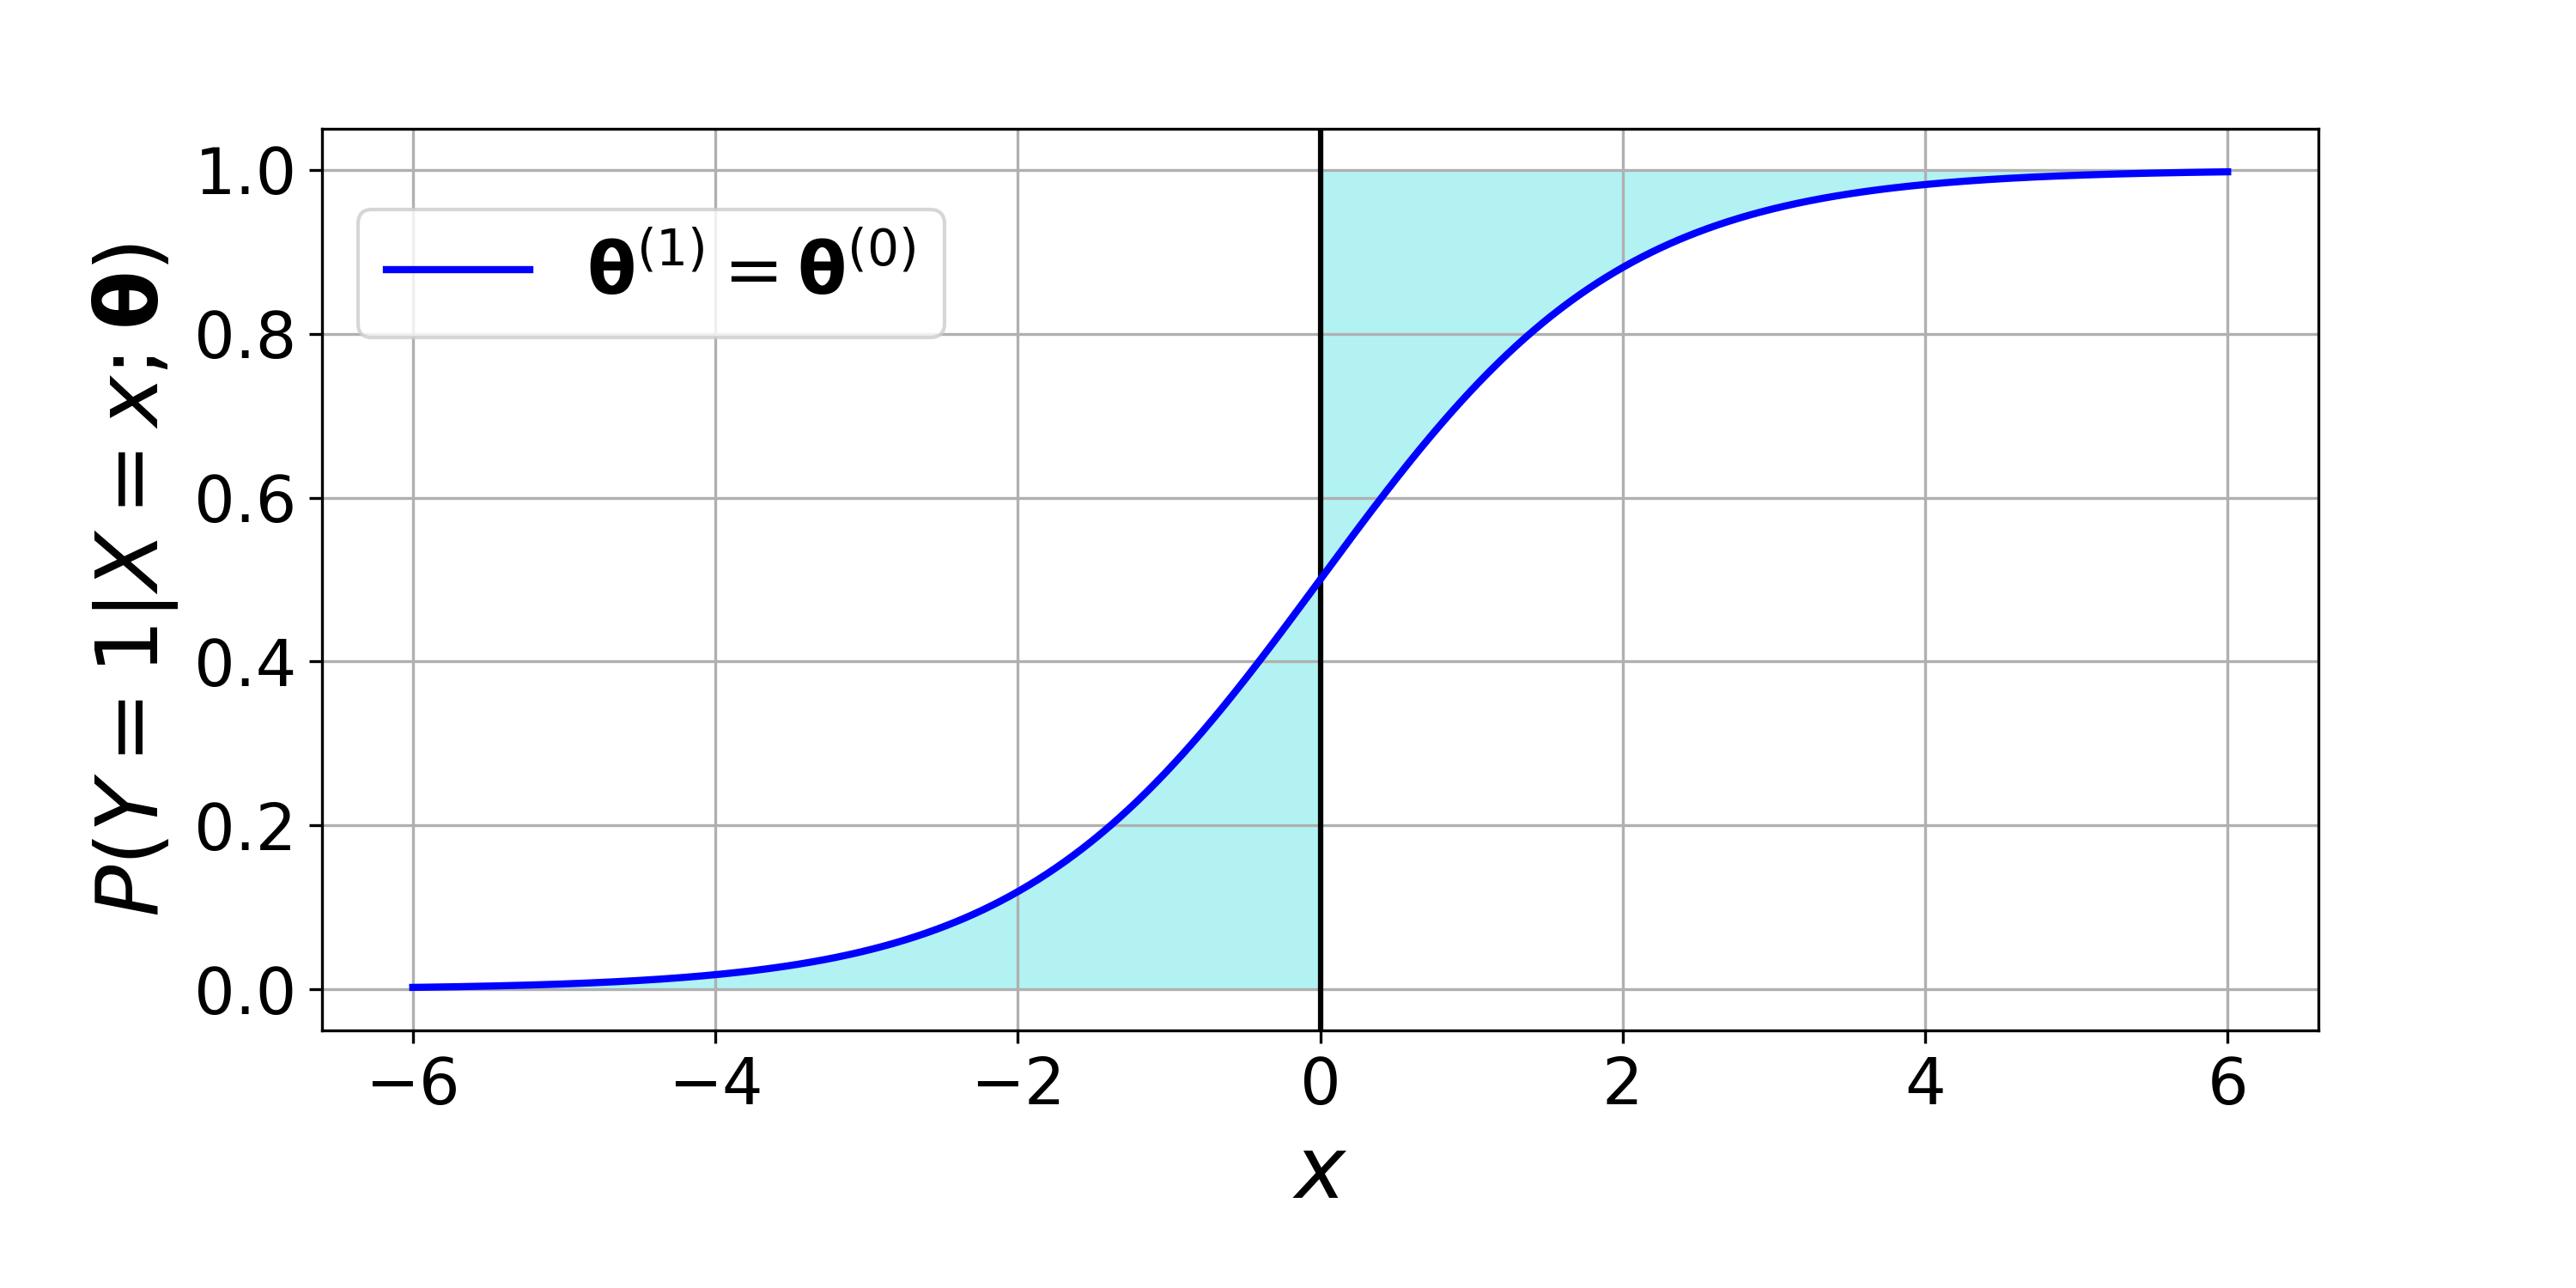
\includegraphics[width=\textwidth, trim=.2in .2in .7in .45in, clip]{../figures/v14/demons_fig/2D_logi_orig.png}
         \caption{The Original Data generating process and model.}
         \label{fig:logi_err_rate_unch_a}
  \end{subfigure}
  \begin{subfigure}[t]{0.4\linewidth}
         \centering
         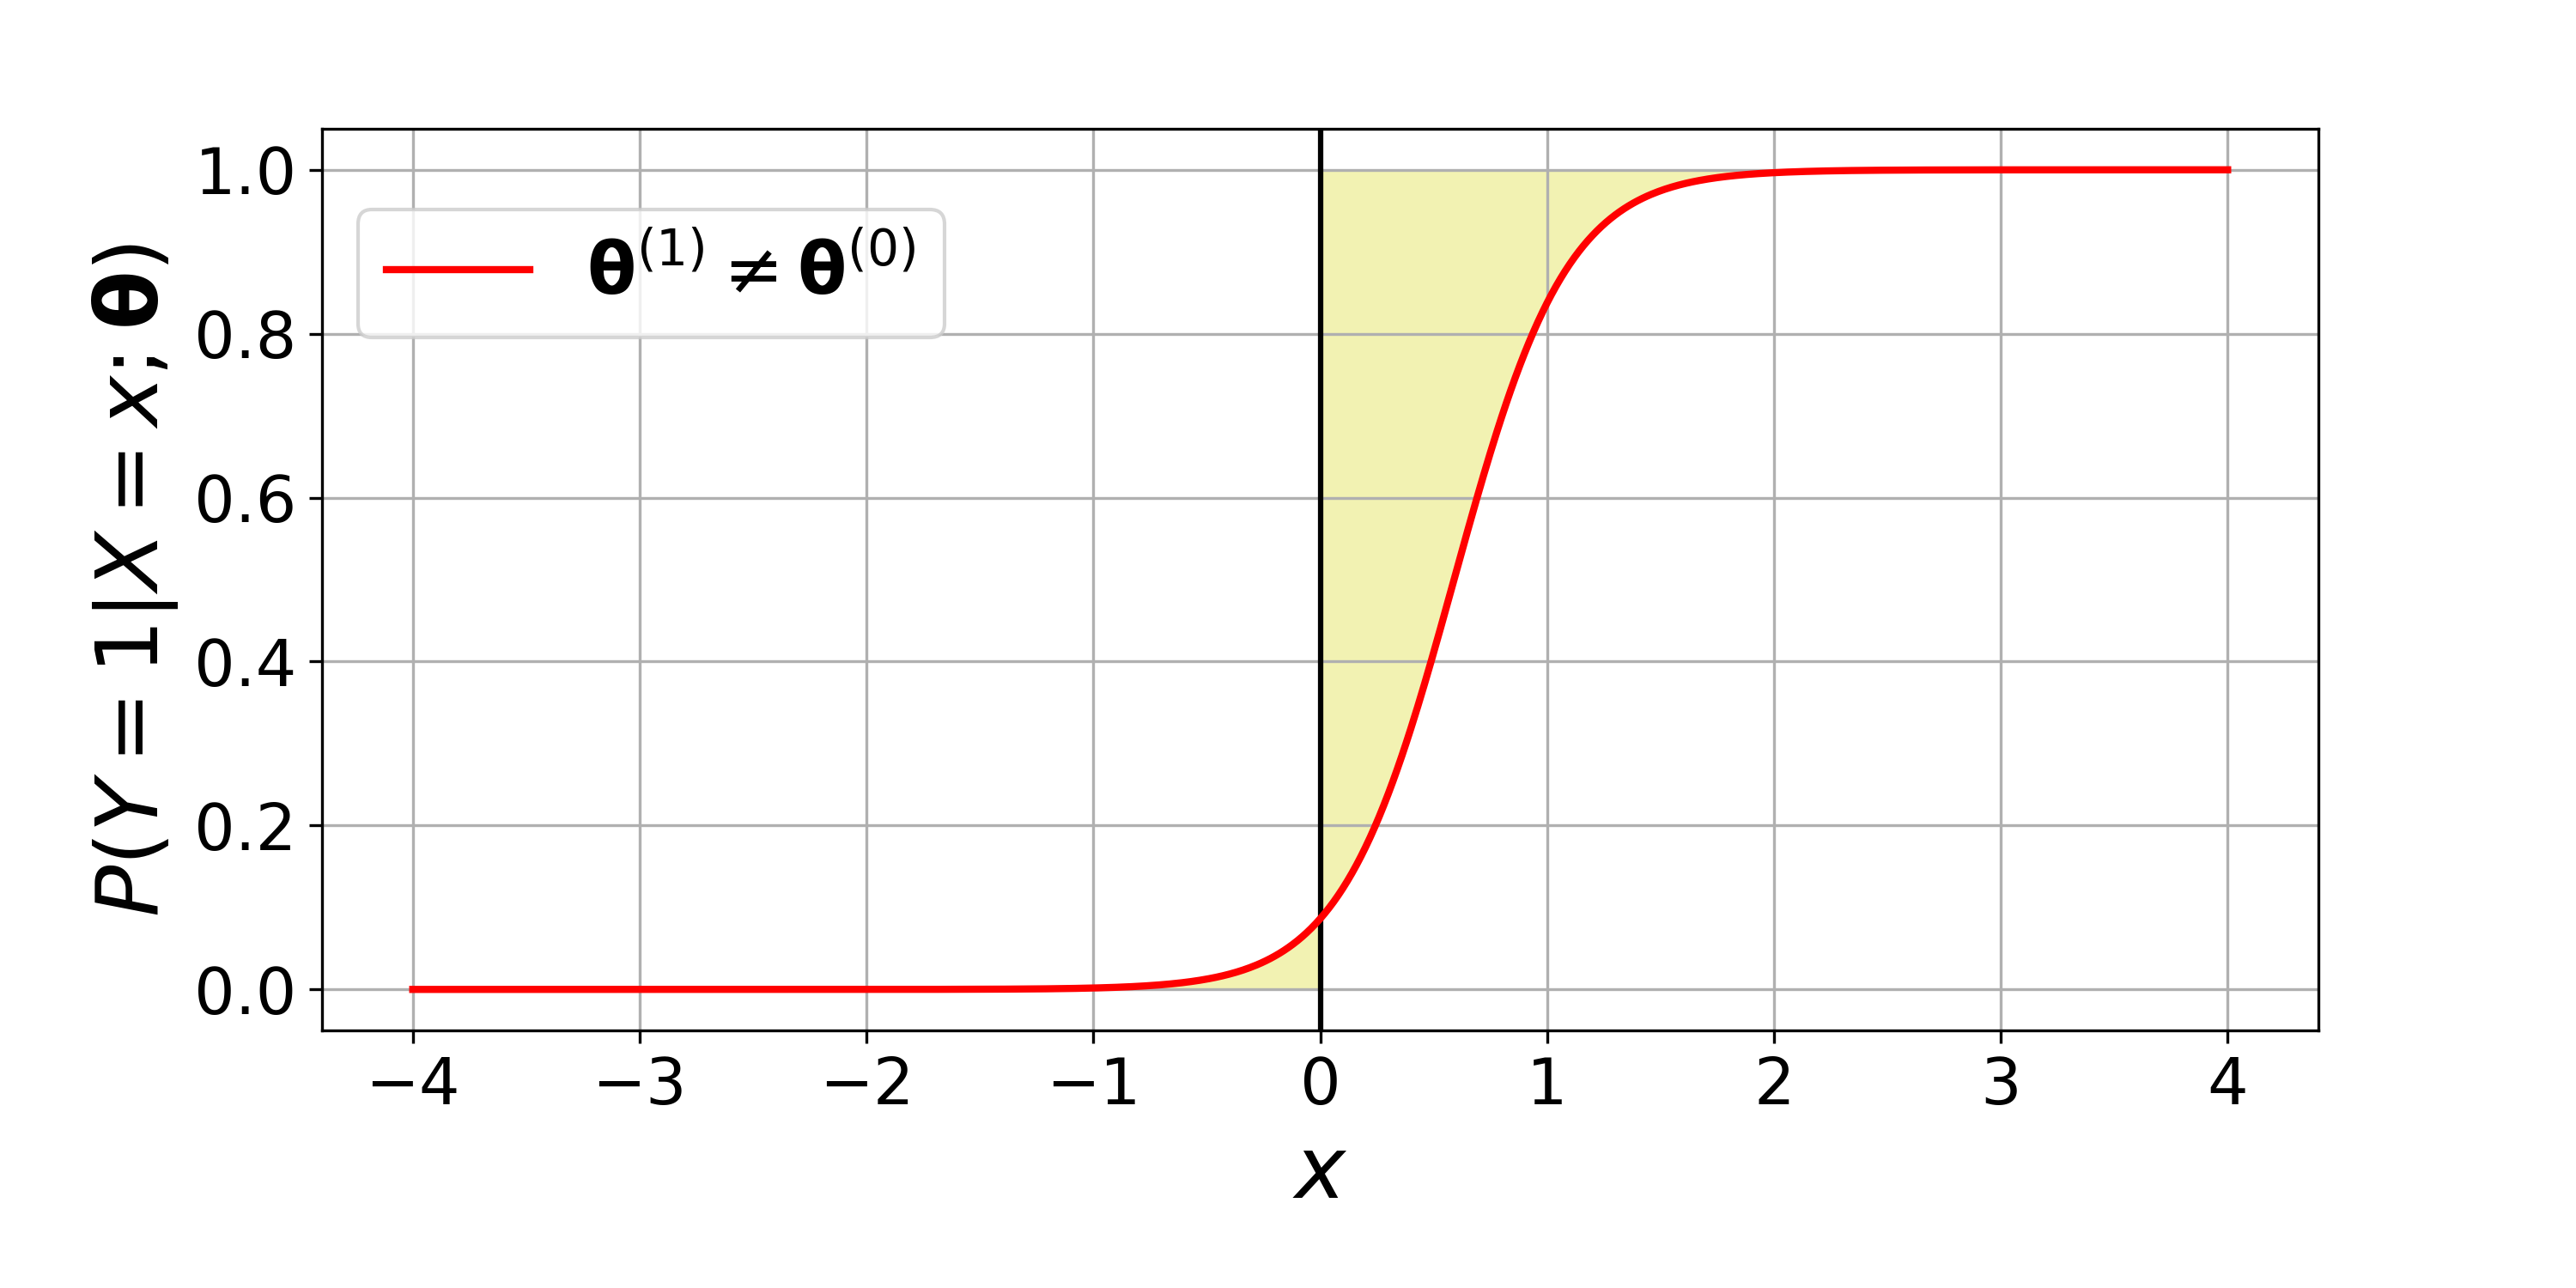
\includegraphics[width=\textwidth, trim=.2in .2in .7in .45in, clip]{../figures/v14/demons_fig/2D_logi_cd.png}
         \caption{The drifted data generating process.}
         \label{fig:logi_err_rate_unch_b}
  \end{subfigure}
%  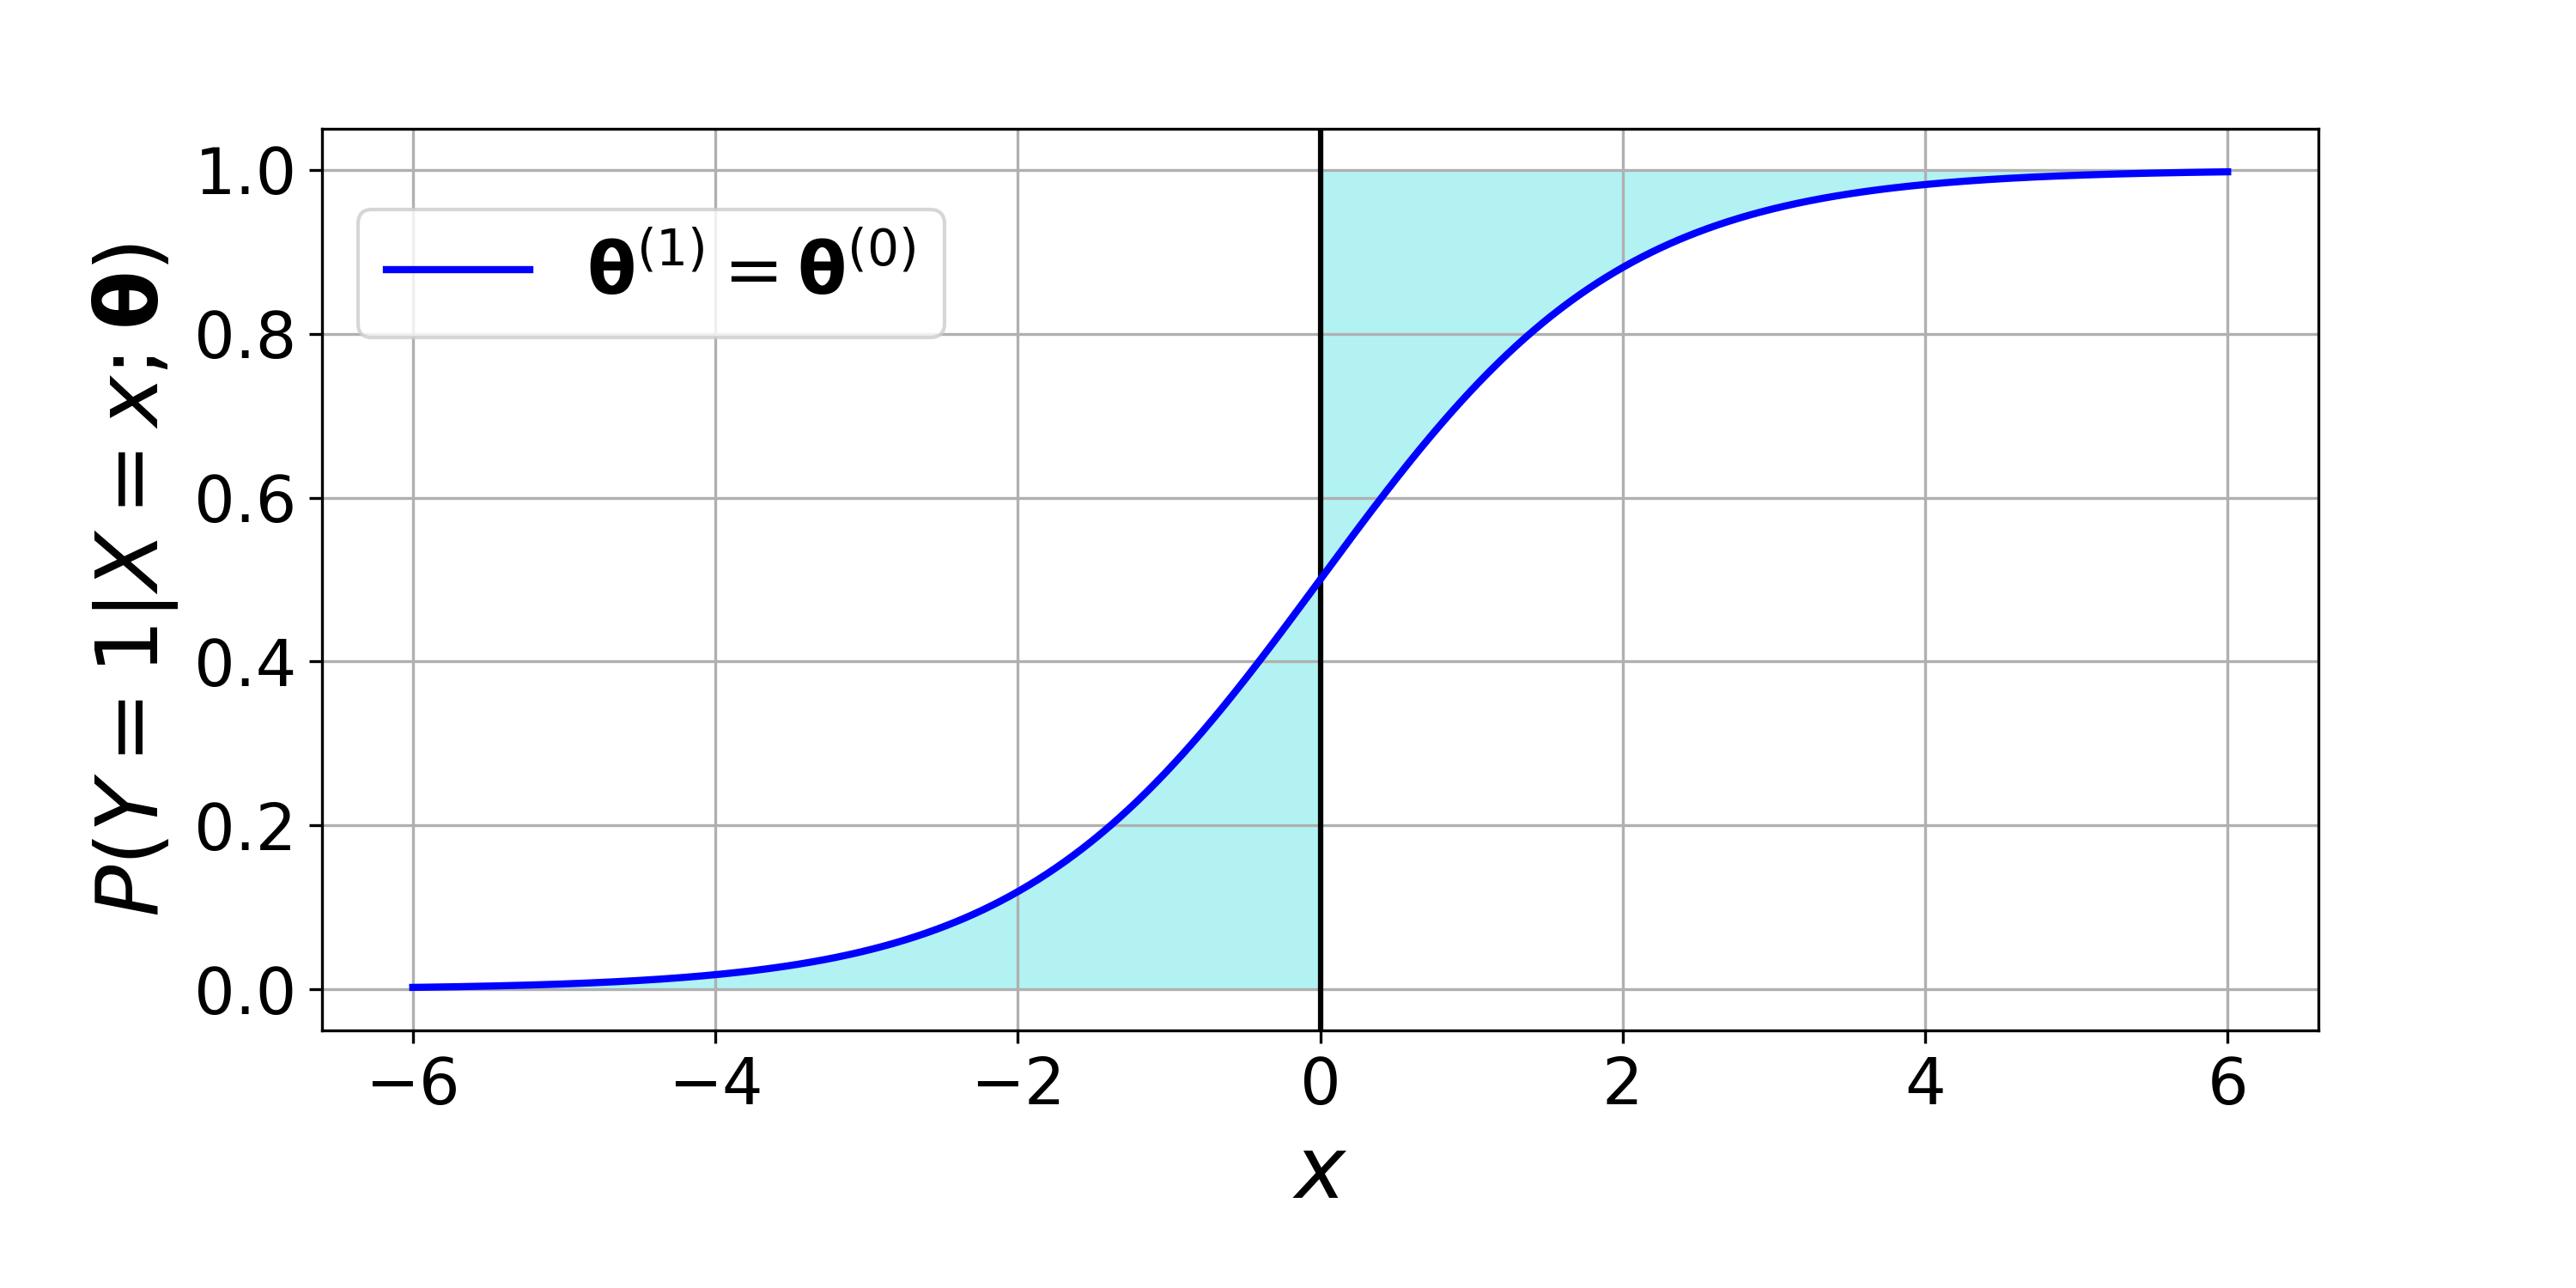
\includegraphics[width = 0.3\linewidth]{../figures/v14/demons_fig/2D_logi_orig.png}
%  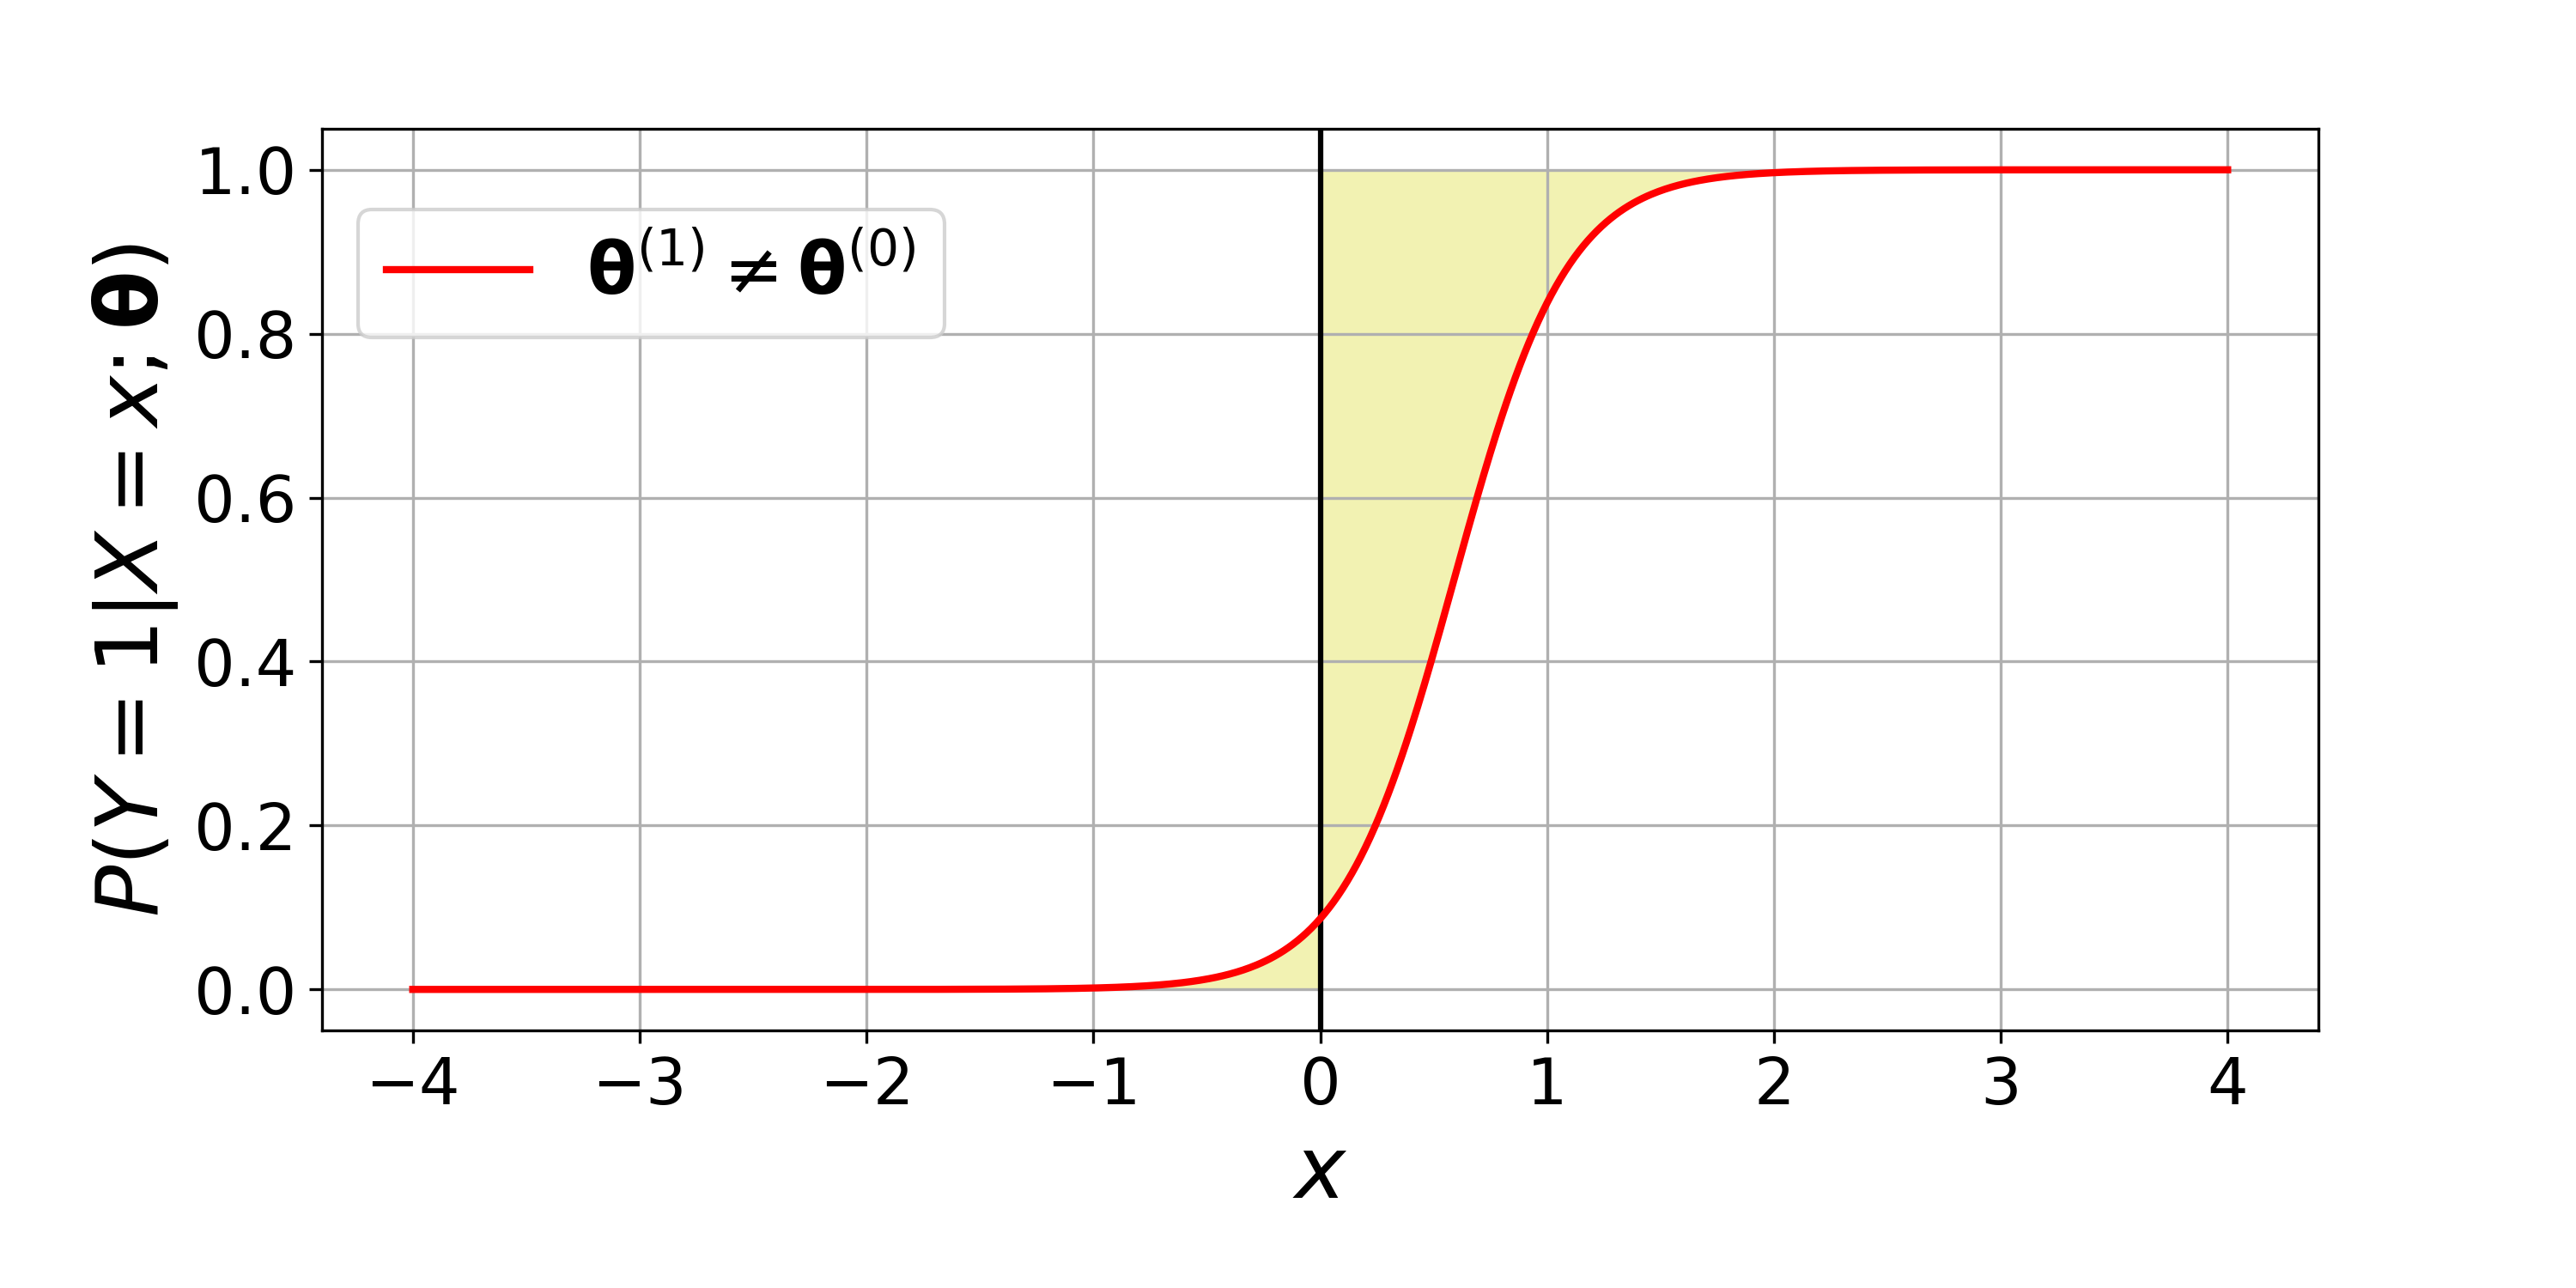
\includegraphics[width = 0.3\linewidth]{../figures/v14/demons_fig/2D_logi_cd.png}
 \begin{subfigure}[t]{0.5\linewidth}
         \centering
	 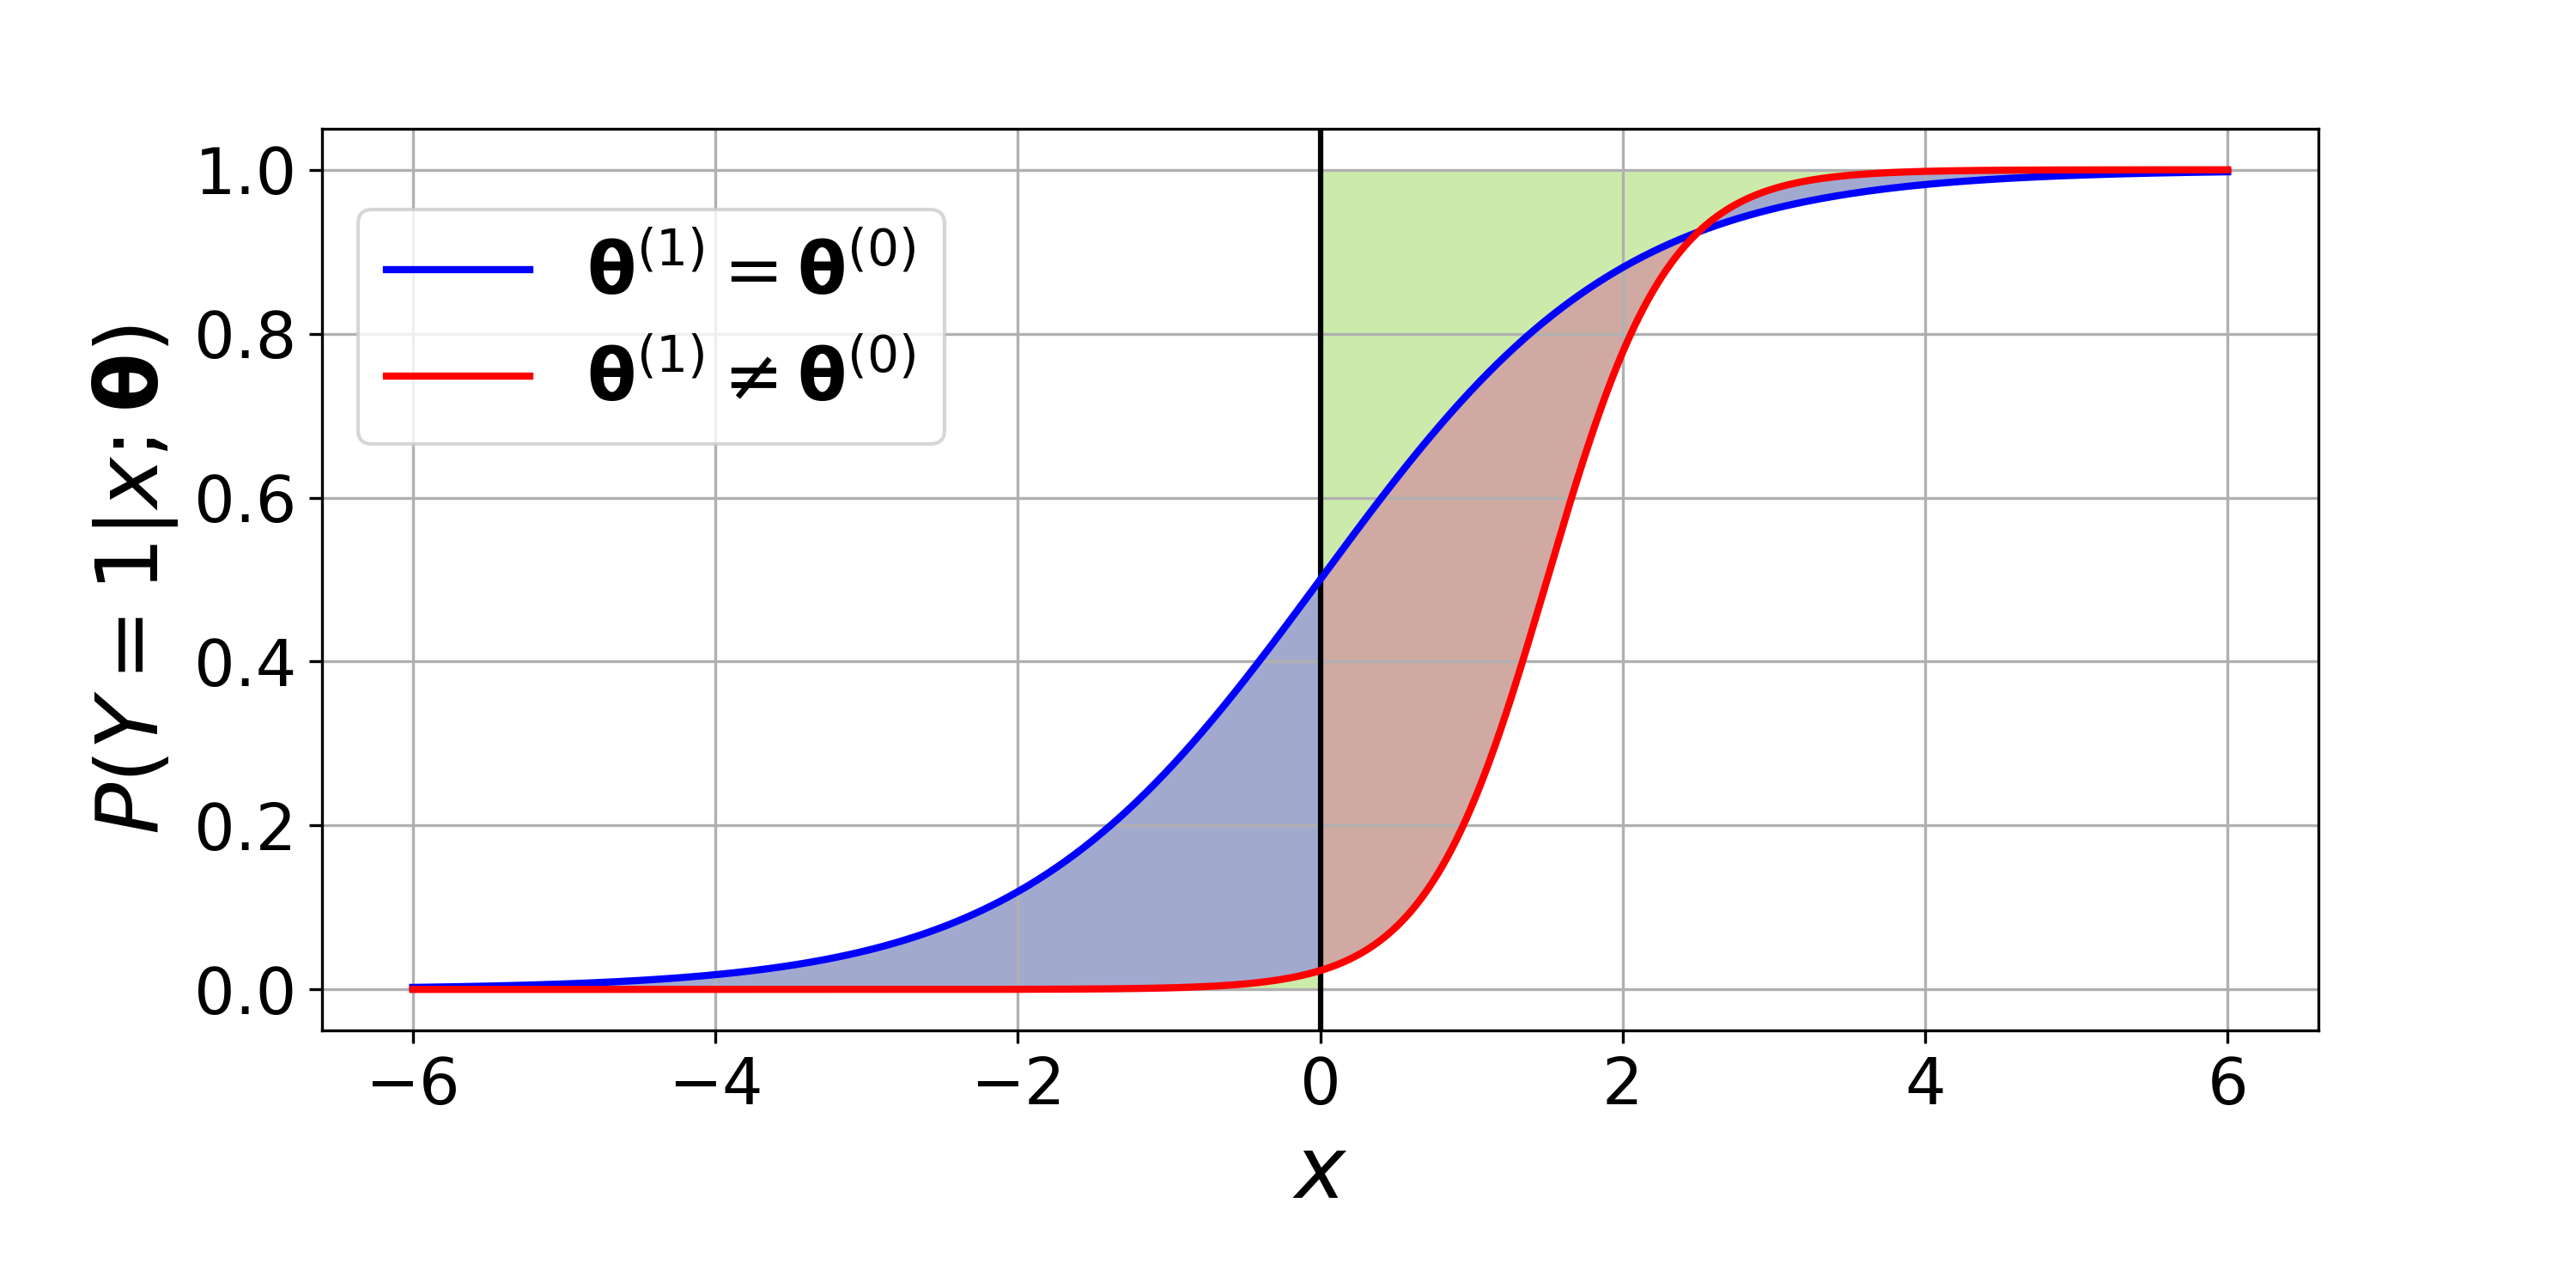
\includegraphics[width = \textwidth, trim=.2in .2in .7in .45in, clip]{../figures/v14/demons_fig/2D_logi.png}
         \caption{The overlap shaded areas from Figure~\ref{fig:logi_err_rate_unch_a} and~\ref{fig:logi_err_rate_unch_b} show unchanged expected error rate.}
         \label{fig:logi_err_rate_unch_c}
  \end{subfigure}
  \caption{The demonstration of simple logistic regression that concept drift would result in no change in expected error rate.}
  \label{fig:logi_err_rate_unch}
\end{figure}

To illustrate the property observed from derivation~(\ref{eqn:exp_score_glm}) in a concrete example, we can construct a logistic regression that concept drift happens without change in error rate, which is defined as indicator function showing whether a prediction equals to true response ($I(\hat {y} \neq y)$). For multinomial regression. The formulas defining the model and the corresponding score function are:
%\begin{align}
%\begin{aligned}
%y=& \bm {x}^T\bm { \theta}^{ (0)}  + \epsilon \\
%\bm{s}(\bm { \theta} ^{(0)};(\bm {X}, Y)) =& (Y - \bm {X}^T\bm { \theta}^{ (0)} ) \bm {X}
%\end{aligned}
%\label{eqn:lin_score}
%\end{align}
%The formula and the score function of logistic regression are:
%\begin{align}
%\begin{aligned}
%p(y=1) =& \sigma ( \bm {x}^T\bm { \theta}^{ (0)} ) \\
%\bm{s}(\bm { \theta} ^{(0)};(\bm {X}, Y)) =&  (Y- \sigma (\bm {X}^T\bm { \theta} ^{ (0)})) \bm {X}
%\end{aligned}
%\label{eqn:logis_score}
%\end{align}
%where $ \sigma ( \cdot)$ is the sigmoid function. The formula and the score function of multinomial regression are:
\begin{align}
\begin{aligned}
\ln (\frac{p_i}{p_0}) = \ln (\frac{p(y=i)}{p(y=0)})&=\bm {x}^{T} \bm { \theta}_i^{(0)}, ~ i \in \{1,2,\cdots,K-1\} \\
\bm {s}(\bm { \theta} ^{ (0)}; (\bm {X}, Y)) &= (\mathbf {Y}-\bm {p})\otimes \bm {X}
\end{aligned}
\label{eqn:multi_score}
\end{align}
where $\bm { \theta} ^{ (0)}$ is generated by stacking all $ \bm { \theta}_i ^{(0)}, (i=1,2,\cdots,K-1)$; $\bm {p}= [p_1, p_2, \cdots, p _{K-1}]$; $\mathbf {Y}$ is one-hot-coding for $Y$, without the entry corresponding to label $0$; $\otimes$ is the kronecker product. When $K=2$, it reduces to logistic regression. It is straightforward to check that the (conditional) expectations of the score function is $\bm {0}$. More complex models like regression or classification with neural network also have a score function are similar and skipped here. 

As shown in the Figure~\ref{fig:logi_err_rate_unch}, the blue solid line is the original model where binary data are generated according to Bernoulli distribution at each horizontal position $x$. We assume that the trained model almost perfectly captures the original model, so that the decision boundary is the $x=0$ (assuming the distribution of $x$ is a truncated normal over $[-6, 6]$). After concept drift, the data generating model becomes the red line, where the optimal decision boundary has been changed. Error rate of the logistic regression model given predictor $\bm {X}$ can be written as a function (we call it ``penalty function" to help explanation):
\begin{align}
C _{err}^{(i)}(\bm {X}) = p ^{(i)}I(\hat{y}=0)+(1-p ^{(i)})I(\hat{y}=1)
\label{eqn:penal_err}
\end{align}
where $p ^{(i)} = P(Y=1|\bm {X}; \bm { \theta} ^{(i)})$, ($i=0,1$), and the superscript, $i$, indicates that this probability function is from original distribution under which the model is trained ($i=0$) or the distribution of new samples during prediction (after a decision model being trained, $i=1$). Thus, if concept drift happens after training, $p ^{(1)} \neq p ^{(0)}$; otherwise, they are equal. Notice that the probability function $p ^{(1)}$ and indentity function $I$ depend on predictor vector $\bm {X}$, but omitted for clean notation. Given the distribution of covariates $\bm {X}$ and decision rule (model) $\hat{y}$, the expectation of this penalty function are those shaded areas in the Figure~\ref{fig:logi_err_rate_unch_a} and \ref{fig:logi_err_rate_unch_b} for the original (blue) and the drifted (yellow) data generating process. In the Figure~\ref{fig:logi_err_rate_unch_c}, Figure~\ref{fig:logi_err_rate_unch_a} and~\ref{fig:logi_err_rate_unch_b} are overlapped together. The drifted data generating process decreases the error by those blue shaded area but adds the red shaded area as new error. Because the two areas are equal, the expected error rate remains the same. If we only monitor the error rate or any metrics derived from it, the concept drift would be missed. More important, this concept drift changes the optimal decision boundary, so that retraining the model can potentially obtain higher accuracy. 

\begin{figure}[!htbp]
\centering
 \begin{subfigure}[t]{0.49\linewidth}
         \centering
         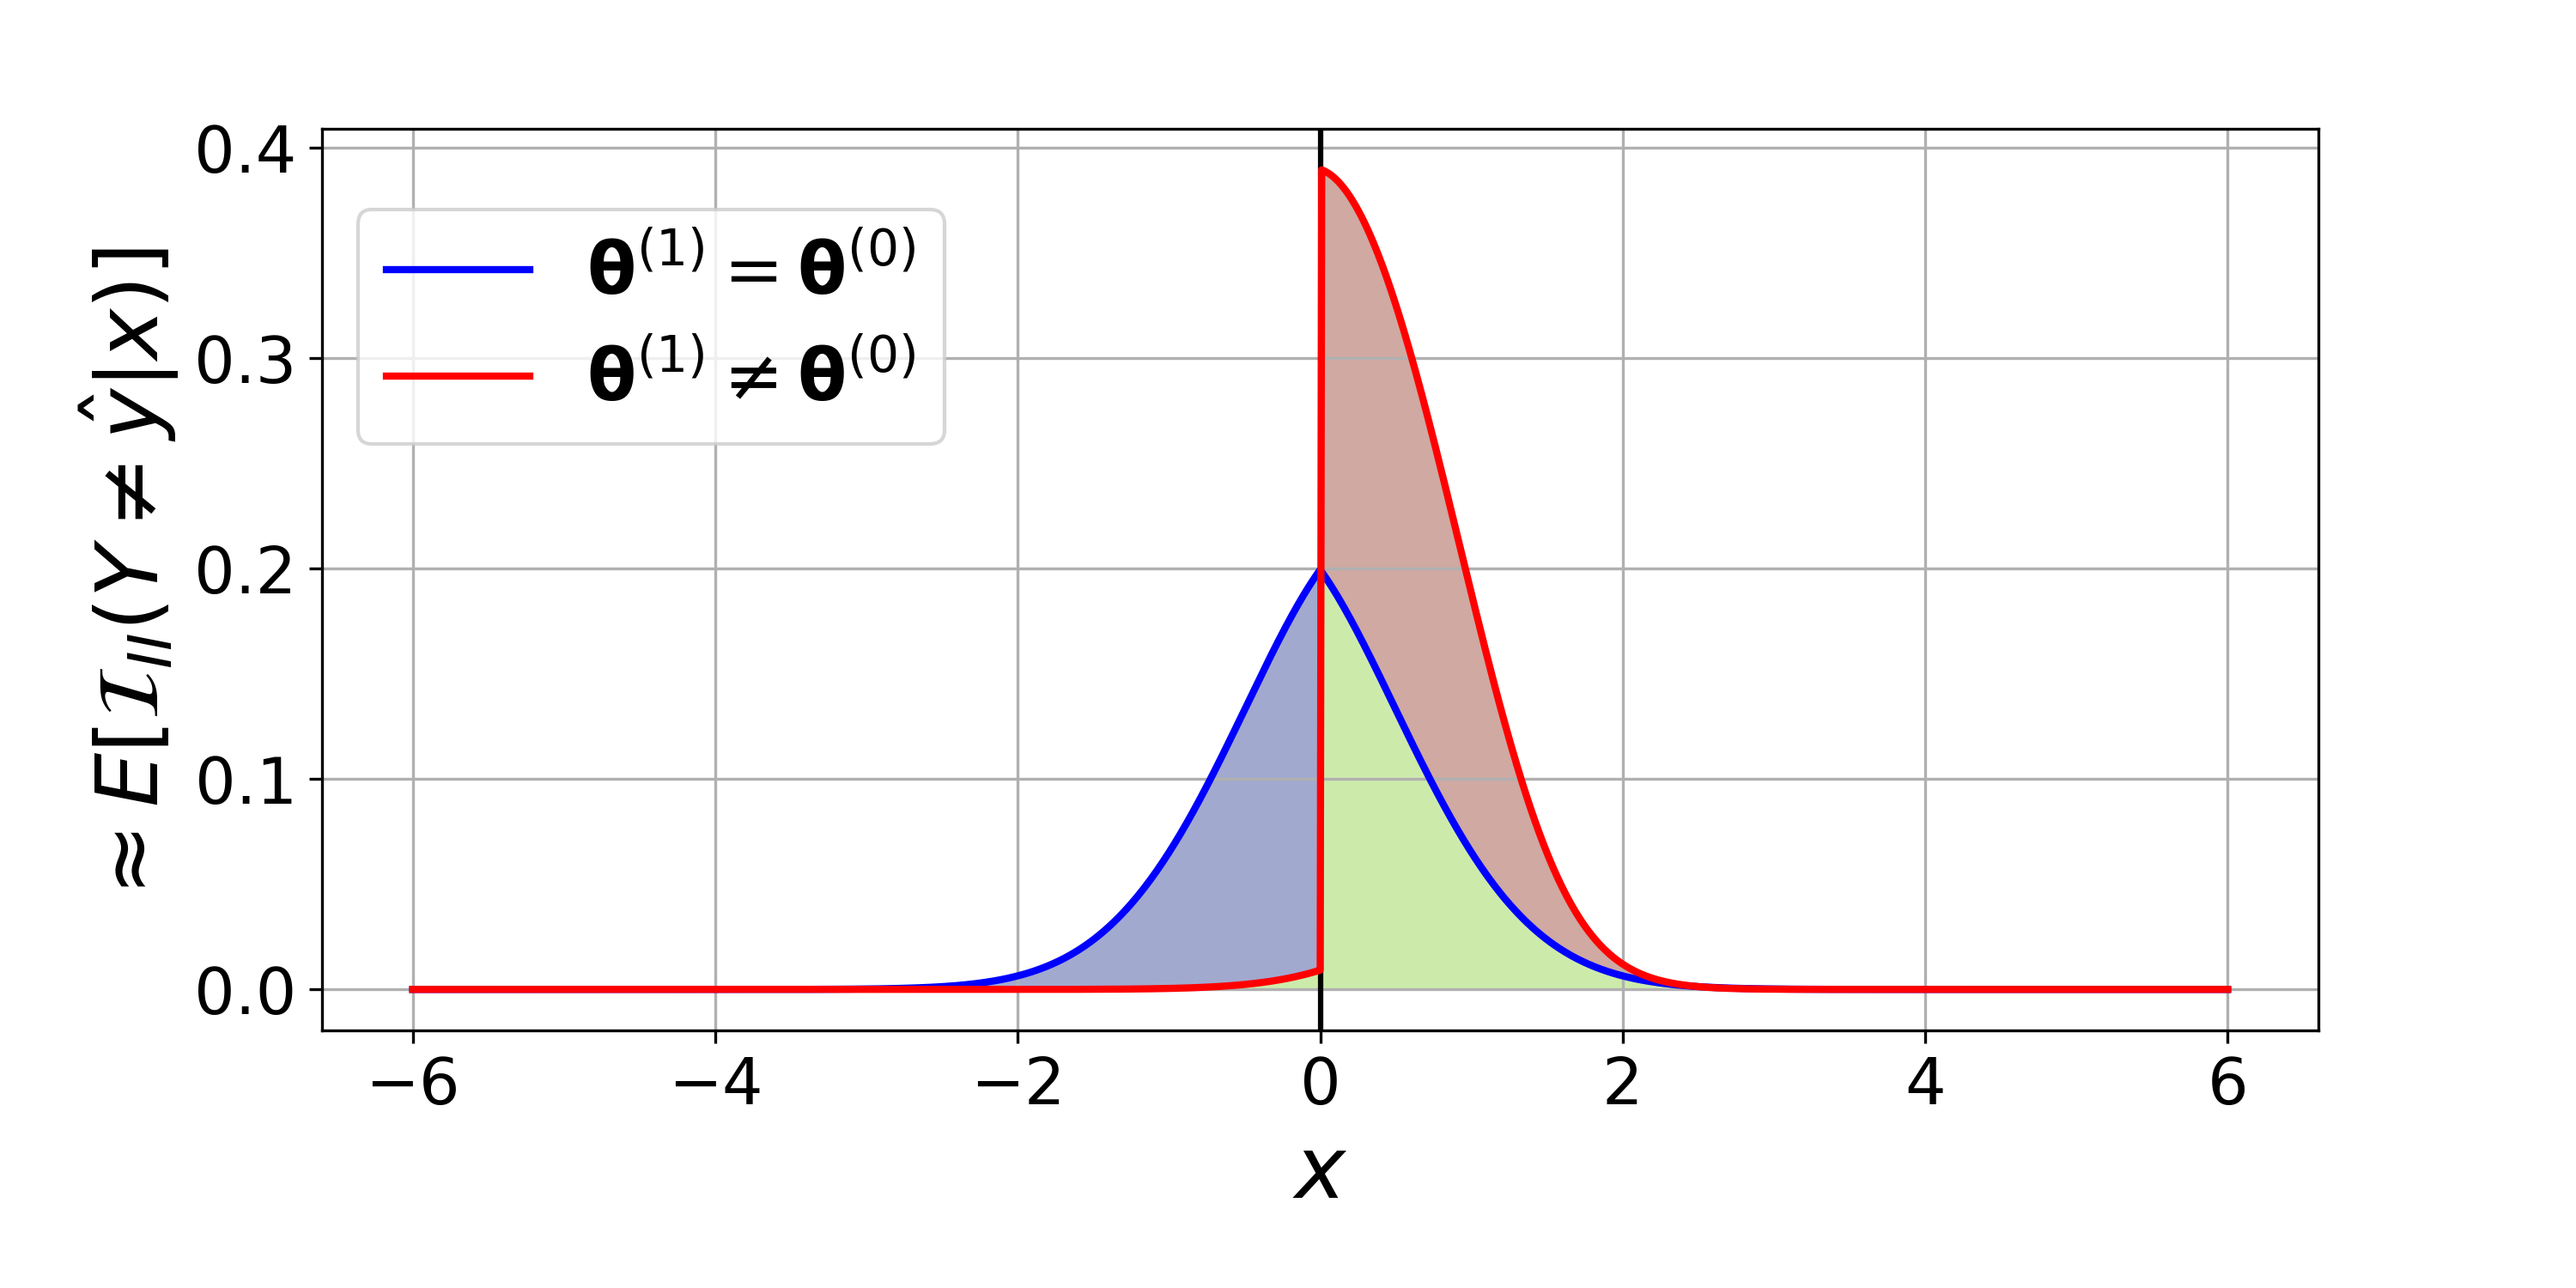
\includegraphics[width=\textwidth, trim=.2in .2in .7in .45in, clip]{../figures/v14/demons_fig/2D_err_logi_trunc_norm.png}
         \caption{The penalty function, equation~(\ref{eqn:penal_err}), before and after concept drift by monitoring error.}
         \label{fig:logi_err_rate_penal}
  \end{subfigure}
%  \begin{subfigure}[t]{0.32\linewidth}
%         \centering
%         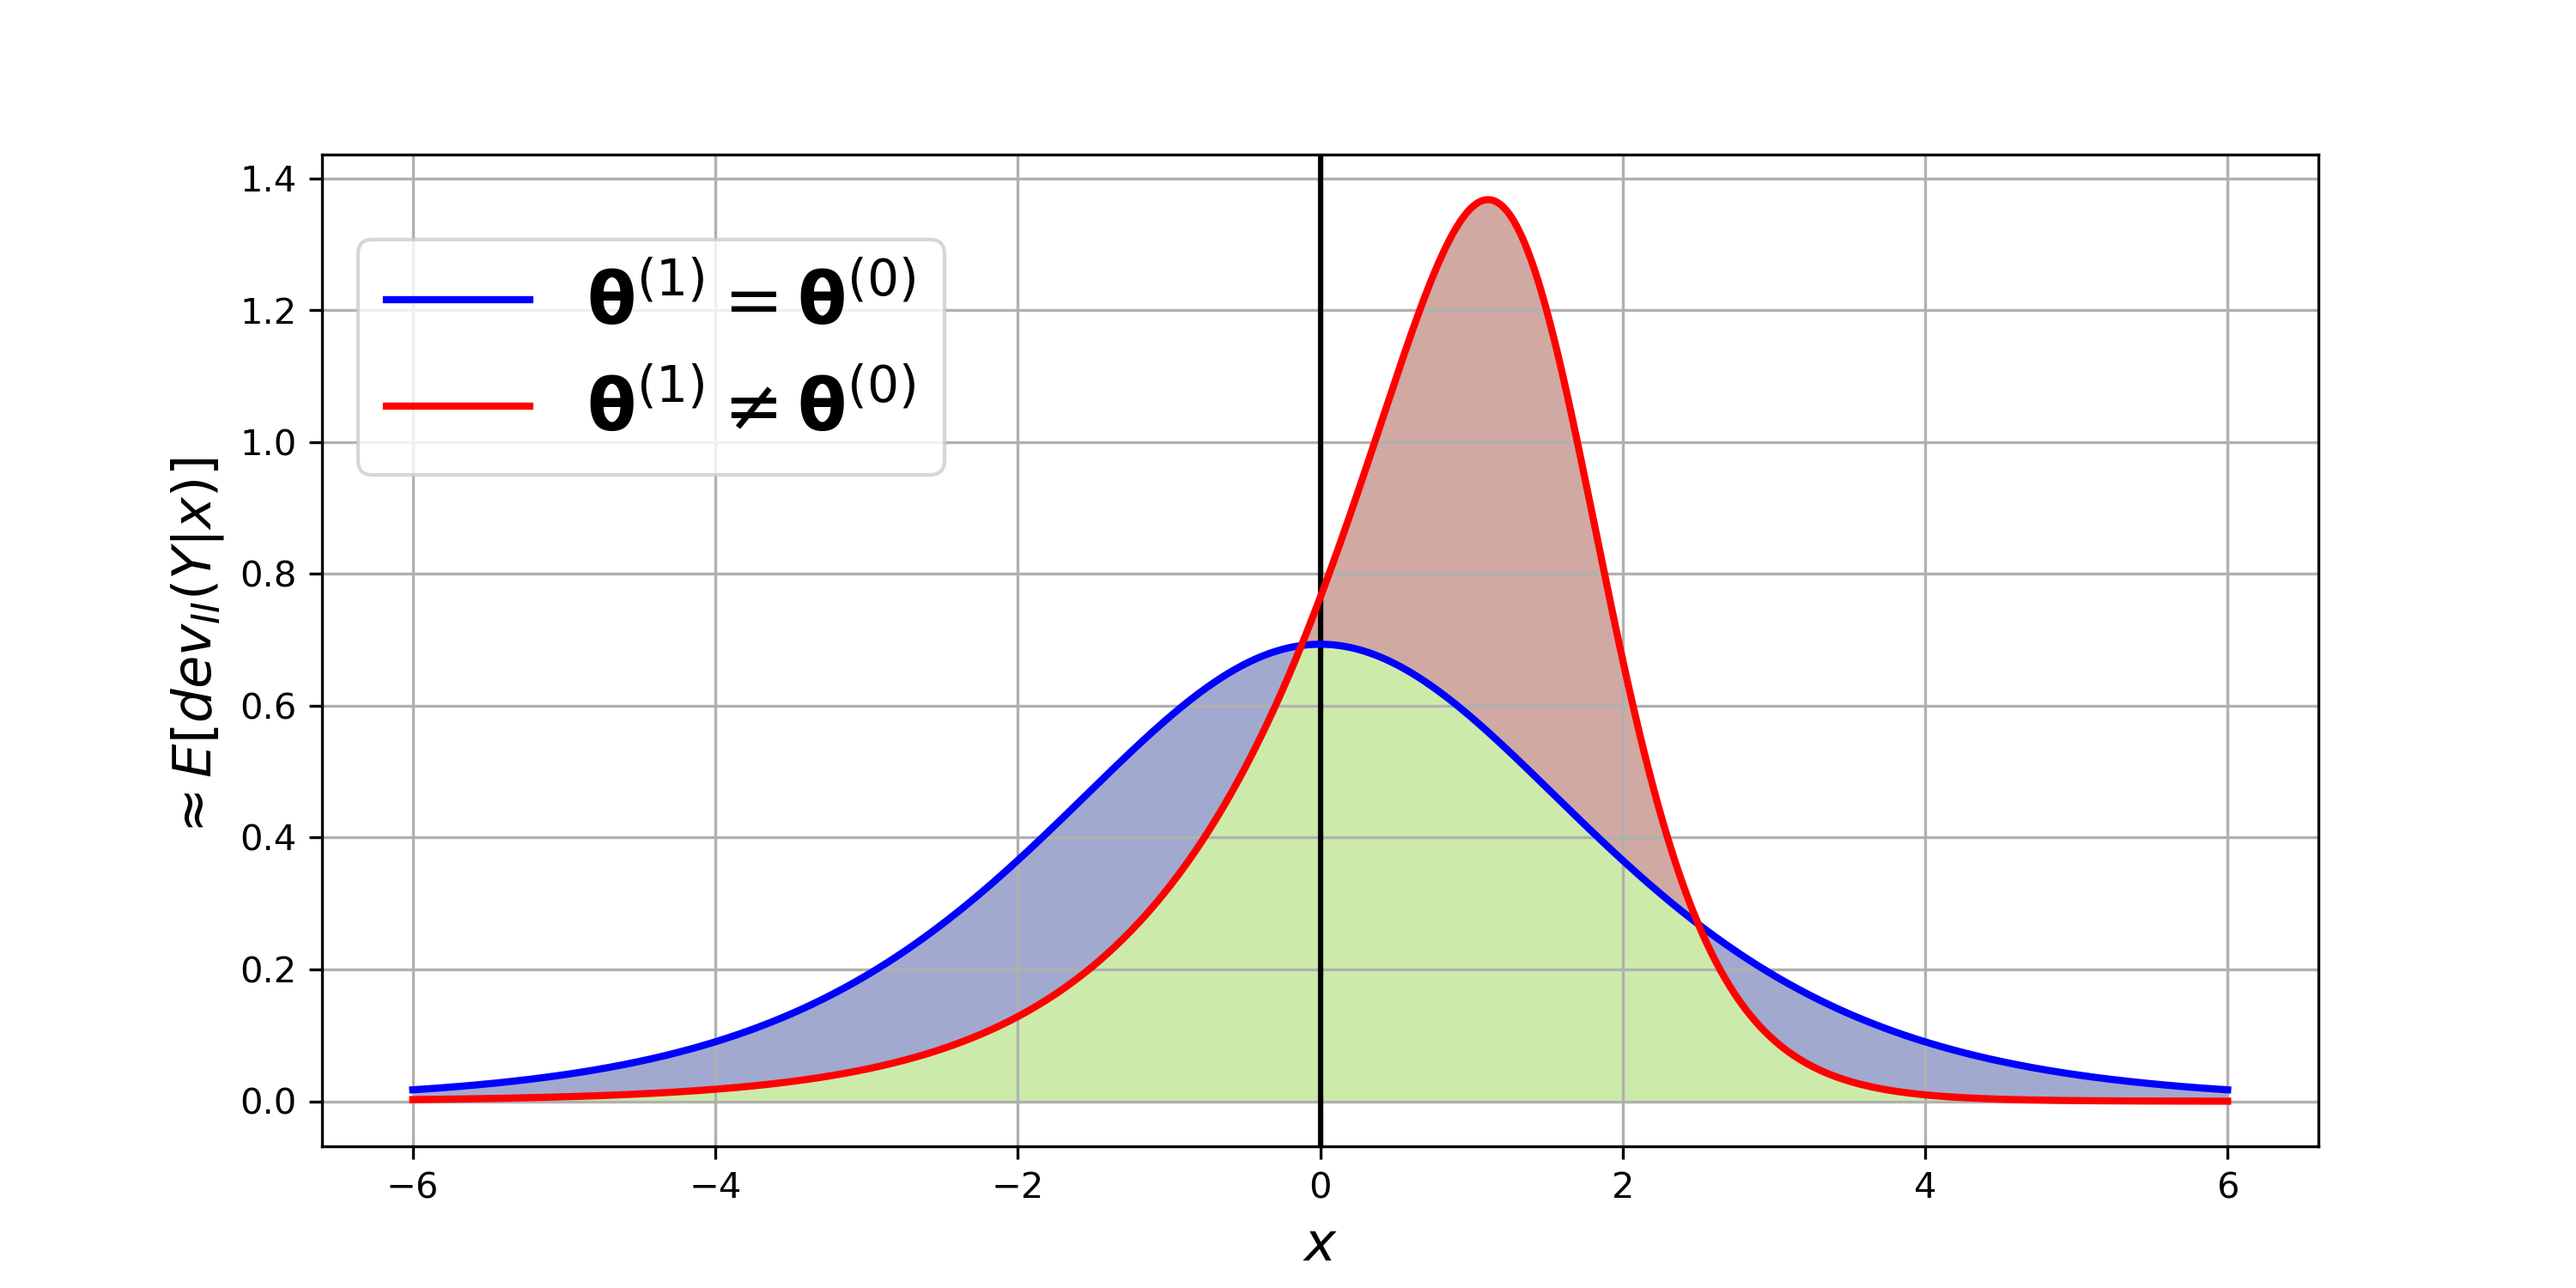
\includegraphics[width=\textwidth]{../figures/v14/demons_fig/2D_dev_logi.png}
%         \caption{The penalty function before and after concept drift by monitoring deviance.}
%         \label{fig:logi_dev_rate_penal}
%  \end{subfigure}
 \begin{subfigure}[t]{0.49\linewidth}
         \centering
% 	 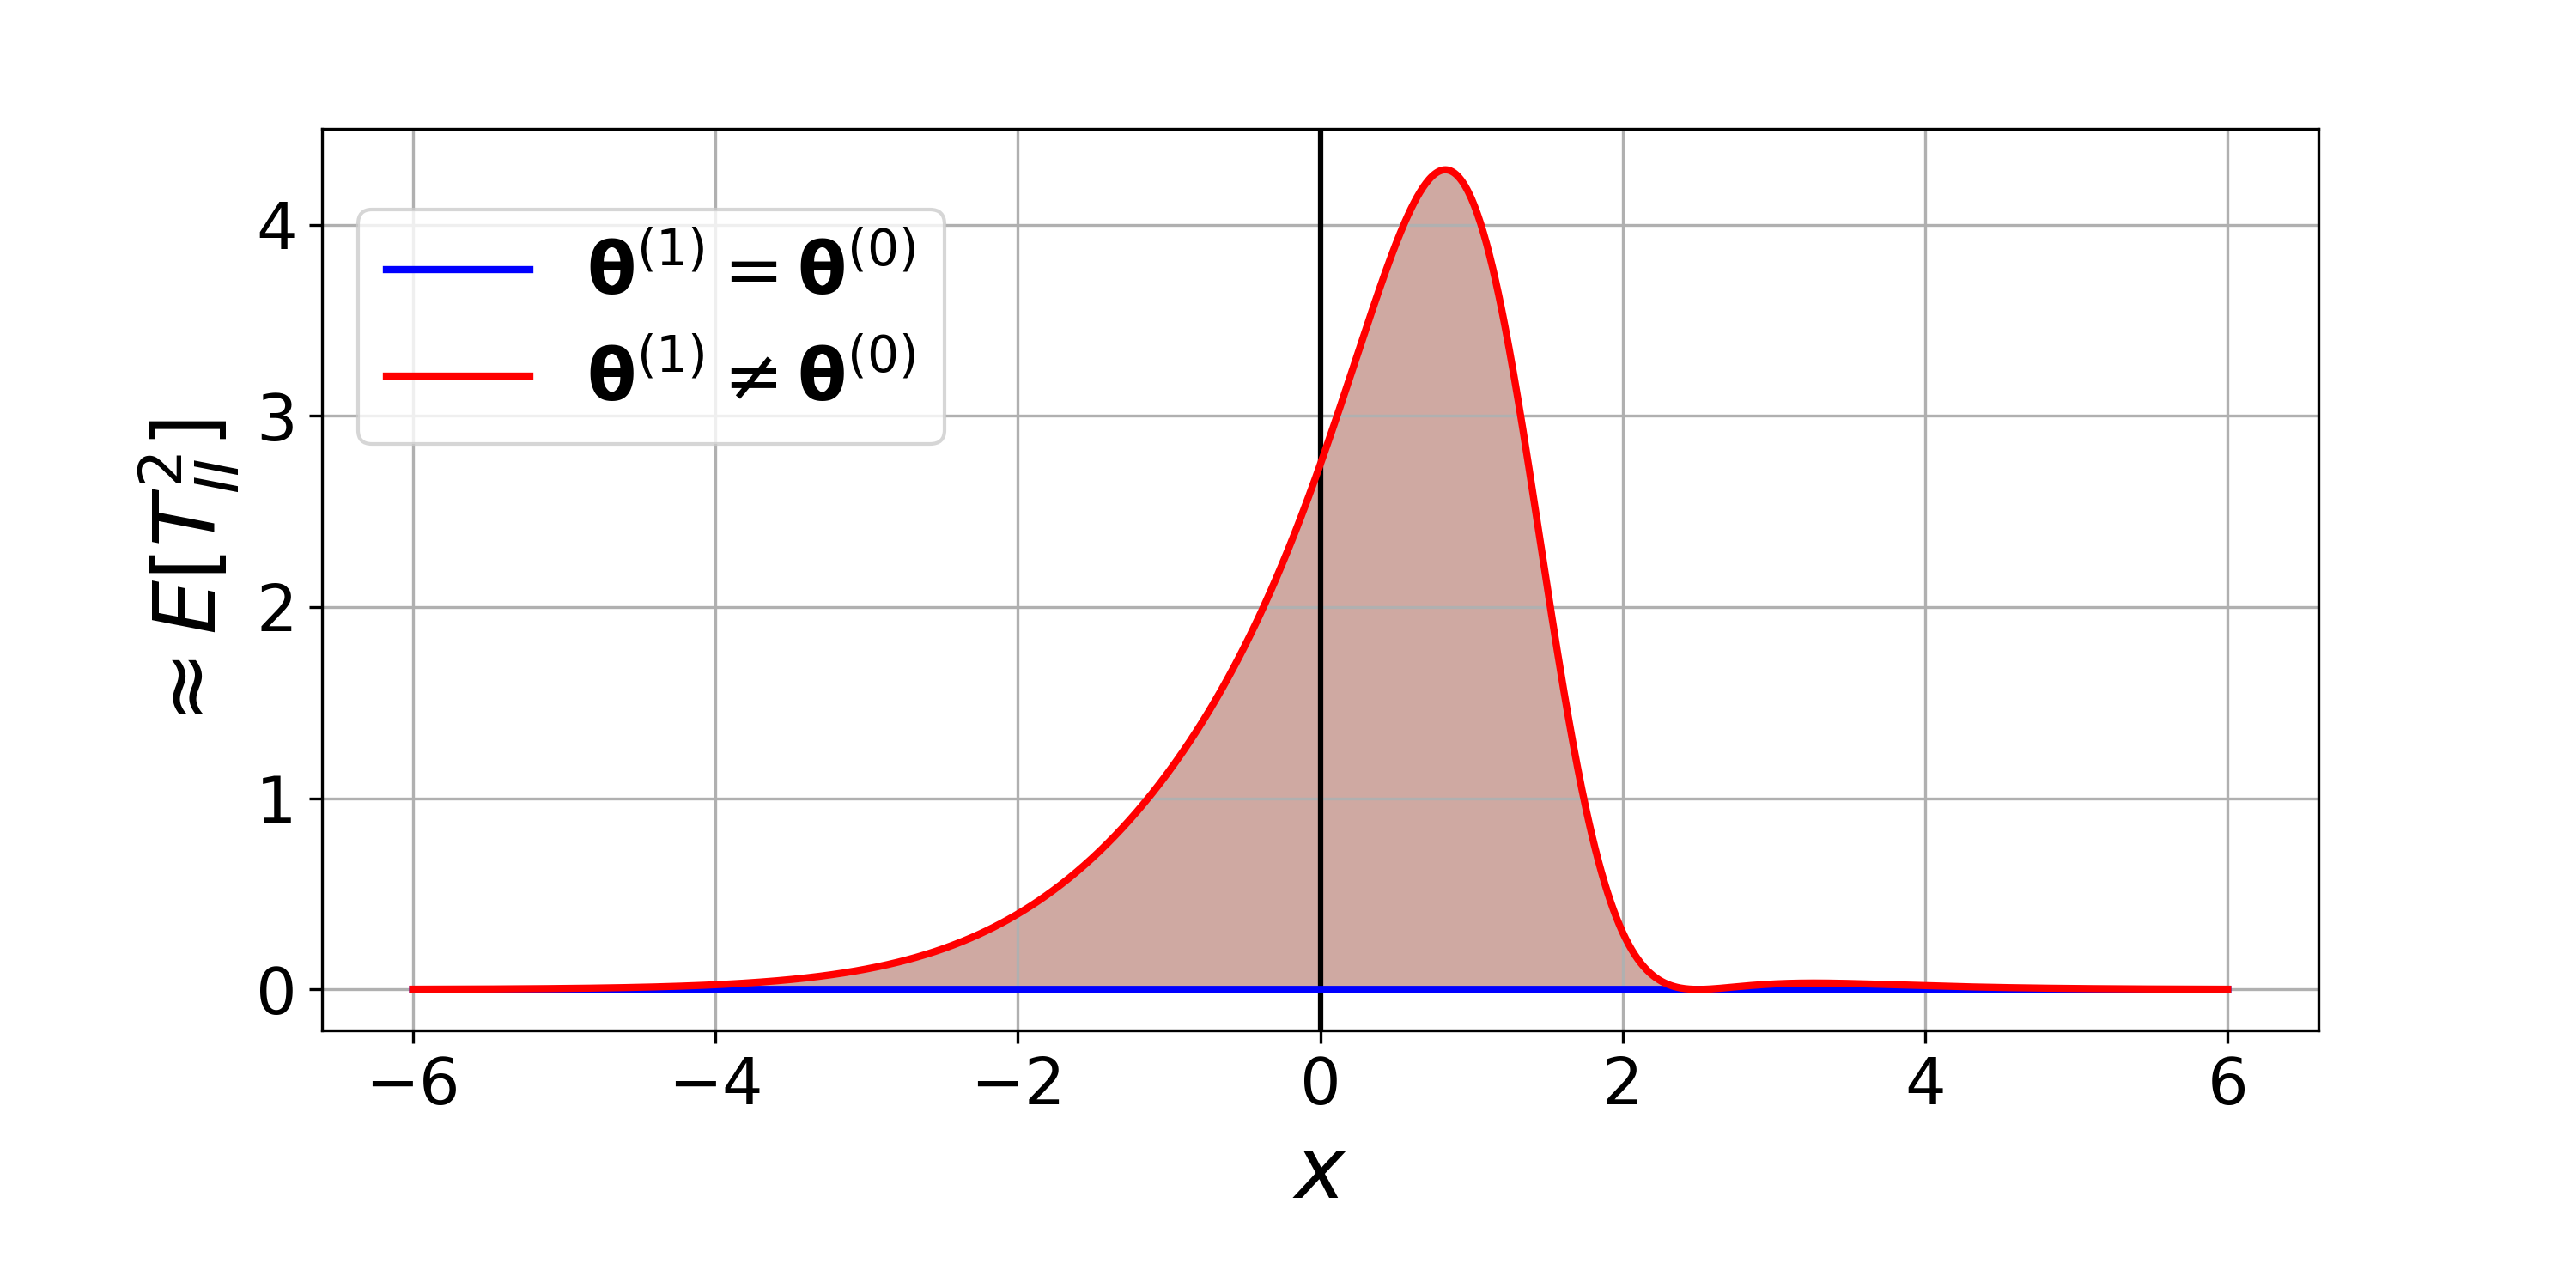
\includegraphics[width = \textwidth, trim=.2in .2in .7in .5in, clip]{../figures/v14/demons_fig/2D_score_logi.png}
    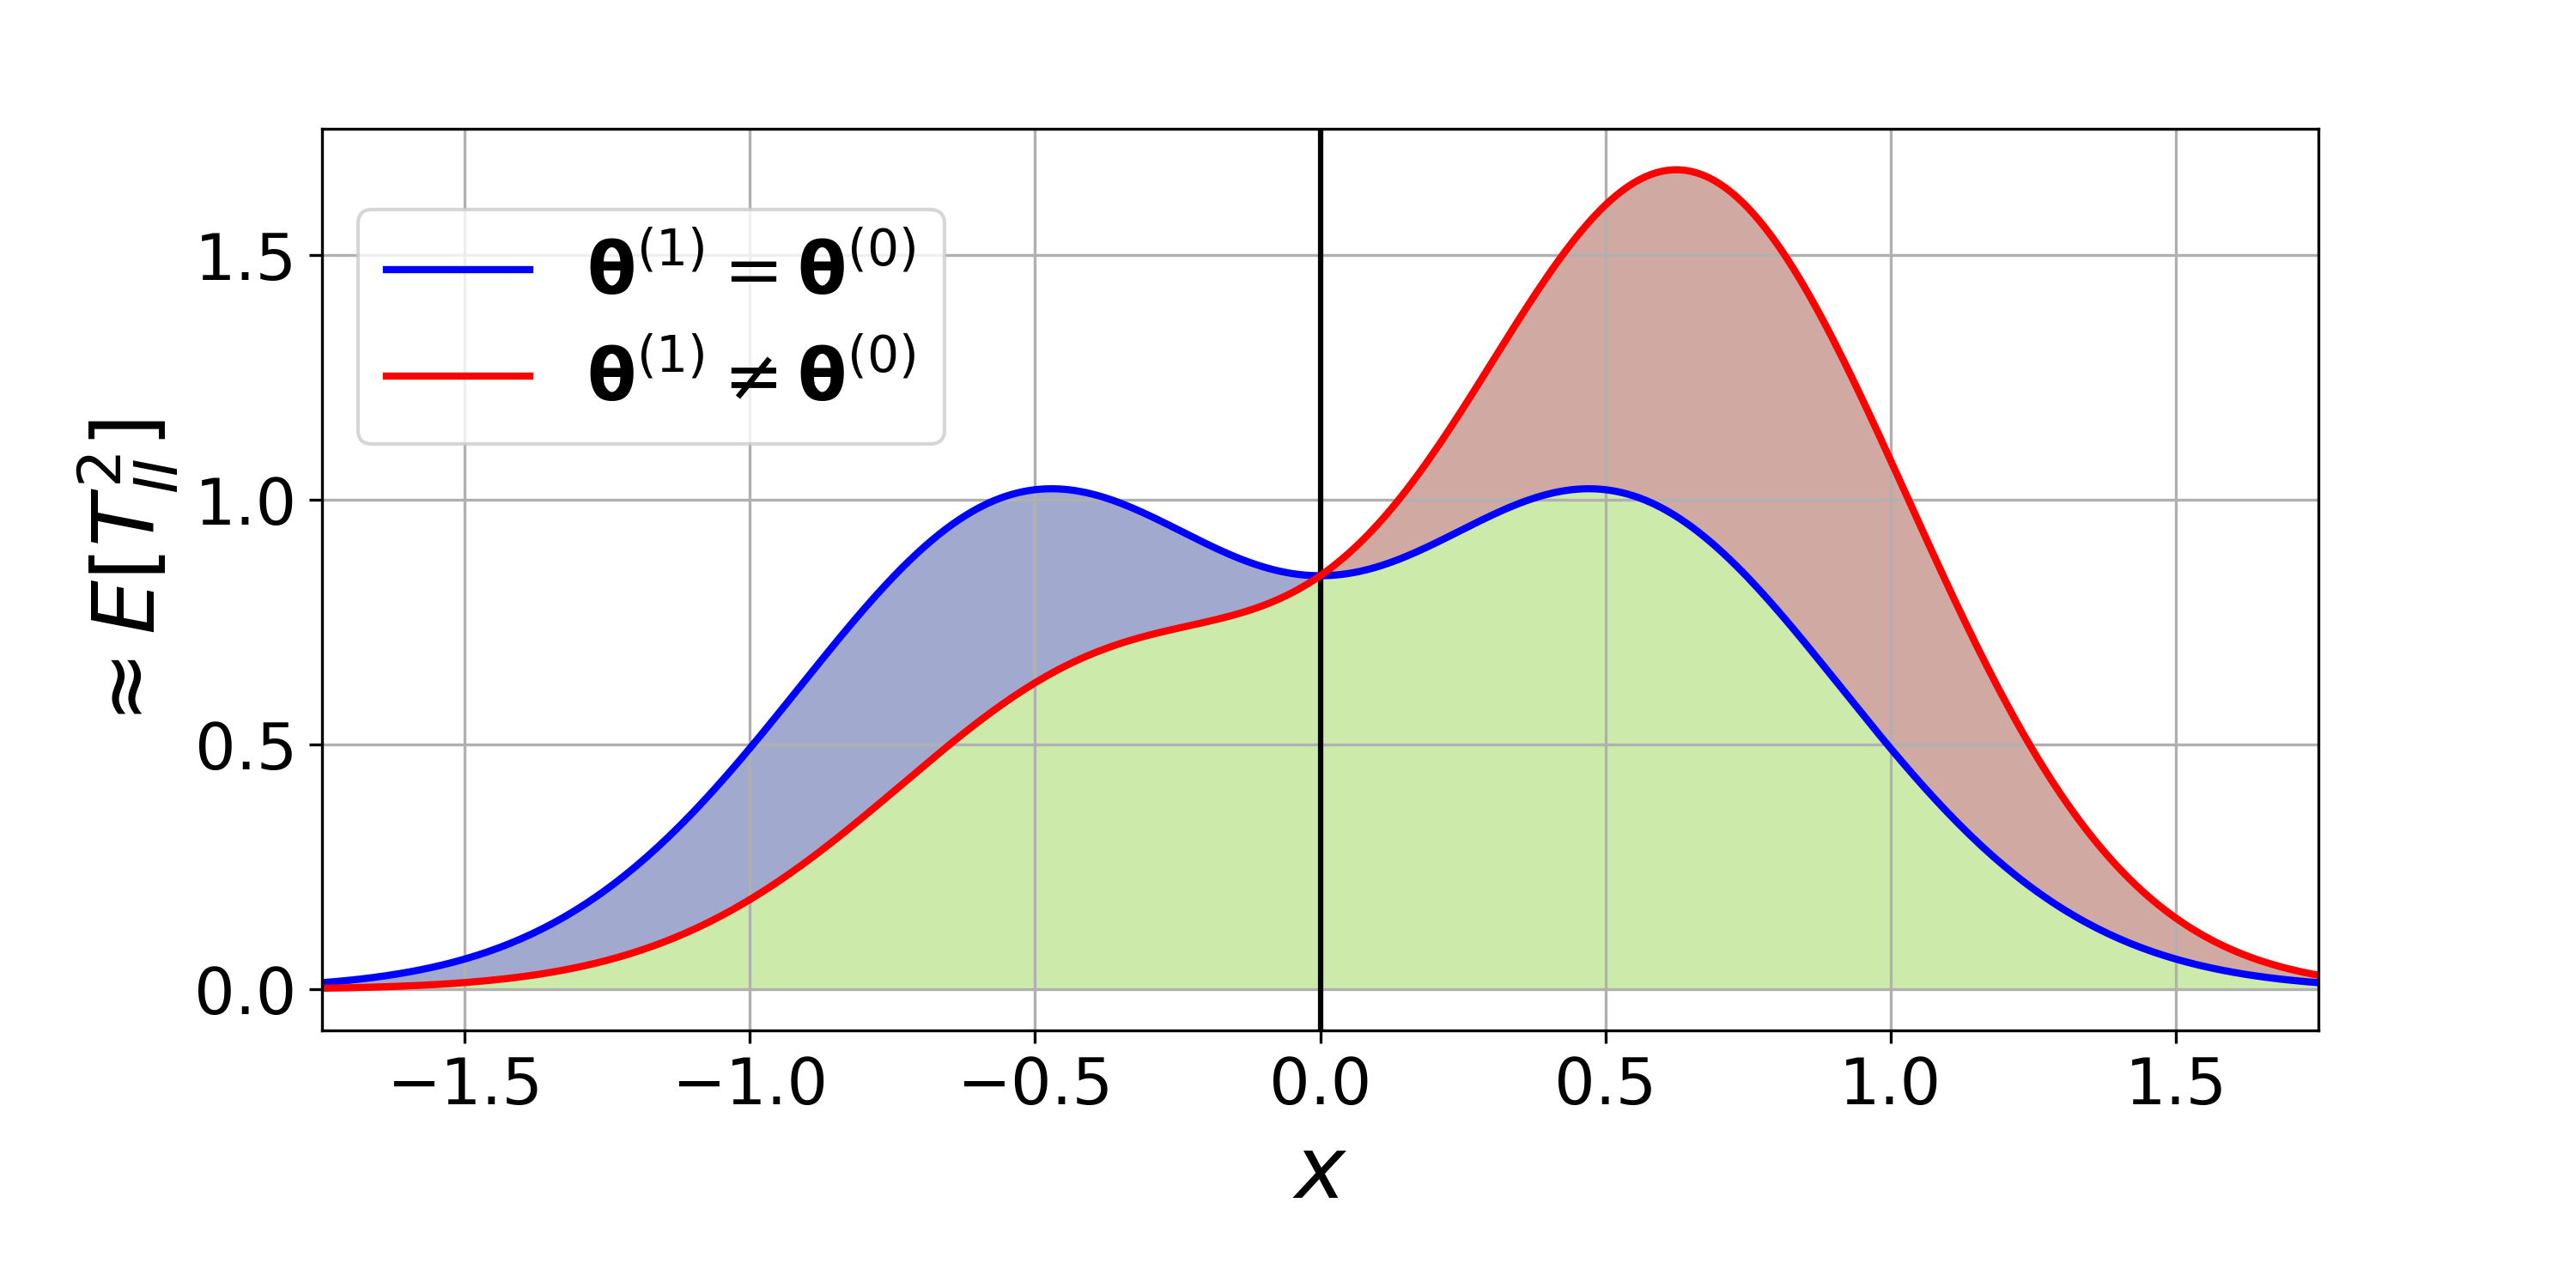
\includegraphics[width = \textwidth, trim=.2in .2in .7in .45in, clip]{../figures/v14/demons_fig/2D_score_logi_modi_trunc_norm.png}
         \caption{The penalty function, equation~(\ref{eqn:penal_score}), before and after concept drift by monitoring Hotelling $T^2$ of EWMA of the score function.}
         \label{fig:logi_score_rate_penal}
  \end{subfigure}
  \caption{The comparison of penalty functions by monitoring classification error and Hotelling $T^2$ of EWMA of the score function.}
  \label{fig:logi_med_penal}
\end{figure}

These plots can be generalized into other penalty functions for metrics like Hotelling $T^2$ of EWMA of the score function as mentioned in the Section~\ref{ss:MEWMA}. For more intuitive comparison, penalties are put close to horizontal line $y=0$, so that the expectation of monitored penalty function equals the area under the curve in Figure~\ref{fig:logi_med_penal}.
%The penalty function for deviance is:
%\begin{align}
%C _{dev}(\bm {X})=-p ^{(1)}\log p ^{(0)}-(1-p ^{(1)})\log(1-p ^{(0)})
%\label{eqn:penal_dev}
%\end{align}
%where $p ^{(0)} = P(Y=1|\bm {X}, \bm { \theta} ^{(0)})$. And 
The penalty function for score function after simplification is:
\begin{align}
C _{score}^{(i)}(\bm {X}) = (p ^{(i)} (1 - p ^{(0)}) + p ^{(0)}(p ^{(0)}-p ^{(i)})) \bm {X}^T\bm { \Sigma}^{-1}\bm {X}
\label{eqn:penal_score}
\end{align}
where $\bm { \Sigma} = E _{\bm {X}}[p ^{(0)}(1-p ^{(0)})\bm {X}\bm {X}^T]$ is the covariance matrix of the score function of the logistic model under training distribution, and the subscript of the expectation means it is over the distribution of covariates $\bm {X}$. As we can see in Figure~\ref{fig:logi_med_penal}, after concept drift, error has the decreased part (blue shaded area) and increased part (red shaded area), which are approximately equal. However, the Hotelling $T^2$ of EWMA of the score function has the increased part larger than the decreased part resulting in net positive change in the penalty function of score function, which indicates that it is more sensitive for monitoring concept drift. The reason is that score function are applied EWMA first and then Hotelling $T^2$. Reversing the order of applying EWMA and Hotelling $T^2$ would void this property, because random noises cannot be averaged out. According to the penalty function~(\ref{eqn:penal_score}) and~(\ref{eqn:penal_err}) and after some derivation, we can see that it makes sense that if two probability functions, $p ^{(0)}$ and $p ^{(1)}$ are different, we have $\int_{\bm{x}}(C _{score}^{(1)}(\bm {x})-C _{score}^{(0)}(\bm {x}))p(\bm{x})d\bm{x}>0$ but the sign of $\int_{\bm{x}}(C _{err}^{(1)}(\bm {x})-C _{err}^{(0)}(\bm {x}))p(\bm{x})d\bm{x}$ is uncertain, which means score-based method directly monitors the deviation of $p ^{(1)}$ from $p ^{(0)}$ while error-based method is not. In other words, score-based method monitors exactly the concept drift. Here the simple logistic regression gives an intuition why score function performs better in monitoring concept drift of parametric models. Of course, in detecting the change of mean, noise level would also affect the sensitivity. We leave the discussion of this issue in Section~\ref{s:demon_cd}: a numerical example would be presented to further support analysis here.

\subsection{Stochastic Gradient Descent and Working with Empirical Data}
\label{ss:sgd_score}
With advancement in technologies of data collection, the amount of data available to train models increases significantly and thus the scale of machine learning models becomes larger and larger. Stochastic Gradient Descent (SGD) or mini-batch Gradient Descent solves the computation problem in training those large-scale models, meaning that data and parameters can fit in memory. In SGD or mini-batch Gradient Descent, the gradient of cost function is approximated by using only one data point (or small batches of training data) instead of the entire data set. Or in online setting, only the newly arrived data are used in generating the gradient. Then, in each iteration this gradient is used to update parameters. If the objective function is log-likelihood as the usual cases, sample score vectors can be obtained automatically after taking gradient ($\nabla _{\bm { \theta}} \sum _{i=1} ^{m} \ln P(y_i|\bm {x}_i;\bm{\theta}) = \sum _{i=1} ^{m} \bm{s}(\bm { \theta};(\bm {x}_i, y_i))$, where $m$ is the batch size) in batch learning or making prediction online. For example, prediction for neural networks requires forward-propagation and another backward-propagation would give the score function. The question is whether the estimated parameters obtained using SGD would approximate the ``true" ones, if it ever exists.

It is important to notice that the property of zero-mean of the score function evaluated at the true parameters, $\bm{\theta}^{(0)}$, in the equation~(\ref{eqn:score_exp_zero}) and uniqueness of the true parameter that maximizes the expectation of log-likelihood, $E_{\bm{\theta}^{(0)}}[\log{P(Y|\bm{X};\bm{\theta})}]$, only hold when the model structure is correct. As Professor Box suggested, ``All models are wrong, but some are useful"~(\cite{box1976science})), usually we cannot expect the model structure is true (meaning $\bm{\theta}^{(0)}$ does not exist), because it is just an approximation of the true predictive relationship. If the model structure is not true, the empirical version of equation~(\ref{eqn:score_exp_zero}):
\begin{align}
\begin{aligned}
&\hat{E}_{\hat{\bm{\theta}}^{(0)}}[\bm{s}(\hat{\bm{\theta}}^{(0)};(\bm{X}, Y))] \vcentcolon=\frac{1}{n}\sum_{i=1}^{n}\bm{s}(\hat{\bm{\theta}}^{(0)};(\bm{x}_i, y_i))=\bm{0}\\
&\hat{\bm{\theta}}^{(0)} \vcentcolon= \argmax_{\bm{\theta}}\hat{E}_{\hat{\bm{\theta}}^{(0)}}[\log{P(Y|\bm{X}; \bm{\theta})}]=\argmax_{\bm{\theta}}\frac{1}{n}\sum_{i=1}^n \log{P(y_i|\bm{x}_i;\bm{\theta})}
\end{aligned}
\label{eqn:score_exp_zero_emp}
\end{align}   
still holds, where $\hat{E}$ is sample mean and $\hat{\bm{\theta}}^{(0)}$ is maximum-likelihood estimator (MLE) by maximizing sample mean of the log-likelihood based on the observed data set, $\{(\bm{x}_i, y_i)\}_{i=1}^n$. That is, when we fit a model using MLE, the gradient of the training log-likelihood with respect to the estimated parameters or the sample mean of the scores over training data, $\nabla_{\bm{\theta}}\hat{E}_{\hat{\bm{\theta}}^{(0)}}[\log{P(Y|\bm{X}; \hat{\bm{\theta}}^{(0)})}]\vcentcolon=\nabla_{\bm{\theta}}\frac{1}{n}\sum_{i=1}^n \log{P(y_i|\bm{x}_i;\hat{\bm{\theta}}^{(0)})}=\frac{1}{n}\sum_{i=1}^n\bm{s}(\hat{\bm{\theta}}^{(0)};(\bm{x}_i, y_i))$, is identically zero, even if the model is not the correct structure. So, the estimated, $\hat{\bm{\theta}}^{(0)}$, takes the place of the true, $\bm{\theta}^{(0)}$. Then, if the predictive relationship changes, such that a different set of parameters, $\hat{\bm{\theta}}^{(1)}\neq \hat{\bm{\theta}}^{(0)}$, now give better prediction, the gradient of the log-likelihood, $\nabla_{\bm{\theta}}\hat{E}_{\hat{\bm{\theta}}^{(1)}}[\log{P(Y|\bm{X}; \hat{\bm{\theta}}^{(0)})}]$, should be non-zero mean. Without confusion, in later sections, we assume there is a true set of parameters, $\bm{\theta}^{(0)}$, because we can always translate discussions to the version with the parameters estimated empirically.

In the definition of concept drift for parametric models, we always assume the true parameters for models would not change in stationary environment. Those properties discussed in Section~\ref{ss:score_func} hold under true unknown parameters. In practical, we always work with estimation of the true parameters, e.g., MLE or an estimation obtained from SGD. In other words, the framework of monitoring the score function is derived from population version but what we truly monitor is sample version. A more rigorous discussion related to the consistency of estimated parameters in sample version is followed to understand the gap between them.

In supervised learning, given a likelihood function, consistent estimators, $\hat {\bm {\theta}}$ (e.g. maximum-likelihood estimator (MLE)), can be used to approximate {$\bm { \theta}^{ (0)}$} using the observed data. To make argument rigorous, we actually need to discuss whether $E_{\bm { \theta} ^{ (0)}}[\bm{s}(\hat{\bm { \theta}};(\bm {X}, Y))|\bm {X}]$ (the expectation of the score function evaluated at an estimation, $\hat { \bm { \theta}}$, to the true vector of parameters, $\bm { \theta} ^{ (0)}$) converges to $\bm {0}$. In batch learning setting, the MLE estimator, $\hat { \bm { \theta}}_ {MLE}$, is asymptotically consistent, so that $E_{\bm { \theta} ^{ (0)}}[\bm{s}(\hat{\bm { \theta}} _{MLE};(\bm {X}, Y))|\bm {X}]$ converges to $\bm {0}$ if the score function is smooth enough in terms of $\bm { \theta}$. In SGD setting, the estimation obtained should converge to\footnote{Step sizes meet certain rules according to Theorem 4.7 from~(\cite{bottou2018optimization}).} the one obtained by batch optimization which is essentially the MLE~(\cite{bottou2018optimization}). Thus the estimator, $\hat {\bm { \theta}} _{SGD} $, obtained by SGD algorithm in stationary environment is also asymptotically consistent. Cost functions other than negative log-likelihood can be practically used to train models, but then theoretical guarantee on the score function no longer exists. In general, approximation {$E _{\bm { \theta} ^{ (0)}}[\bm{s}(\hat{\bm { \theta}};(\bm {X}, Y))|\bm{X}] = O (\hat{\bm { \theta}} - \bm { \theta}^{ (0)}) $} and converges to $\bm {0}$ when sample size $n$ goes to infinity. This is basically assuming parameters of the trained model are already very close to the true optimal value. So given an estimator $\hat {\bm { \theta}}$ to the vector of original true parameters $\bm { \theta}^{(0)}$, monitoring the mean {drift} of $\bm{s} (\hat{\bm { \theta}};(\bm {X}, Y))$ directly signals the potential concept drift, within a high-order term, {$O(\hat{\bm { \theta}} - \bm { \theta} ^{ (0)})$.} Moreover, the MEWMA approach explained in Section~\ref{ss:MEWMA} provides a way to distinguish concept drift from such high-order noise.

% Because $E _{\bm { \theta} ^{ (0)}}[\bm{s}(\hat{\bm { \theta}};(\bm {X}, Y))|\bm{X}] = o (\hat{\bm { \theta}} - \bm { \theta}^{ (0)}) $, we should expect that the monitored sample score vectors have sample mean getting increasingly close to $\bm {0}$, as $\hat {\bm { \theta}}$ converging to $\bm { \theta} ^{ (0)}$. Thus, the mean drift of sample score vectors should be monitored after model training entering fine tuning phase, that is, the relative changes of parameters become small.

% According to our knowledge, no literature from the field of concept drift addresses the problem using the score function. The score function has several advantages. First, concept drifts (or change of parameters in the context of this study) guarantees a non-zero mean, while the error (e.g. classification error) does not have such property. Second, it is a vector with dimension of the number of parameters in the model, so that it provides more granular information about potential change of parameters comparing with other scalar metrics. Third, it is independent to specific models or problems so that it is a general method for parametric supervised learning, unlike error-based metrics (e.g., recall, precision, F1 score) exclusively designed for binary classification. The last but not least, when we make prediction on newly incoming data or use mini-batch Gradient Descent or online learning to finely tune parameters of models, the cost function is just a sum of log-likelihood functions of the mini-batch, $\sum _{i=1} ^{m} \ln f(\bm{\theta}; (\bm {x}_i, y_i))$, so that sample score vectors are by-products while taking gradient, $\nabla _{\bm { \theta}} \sum _{i=1} ^{m} \ln f(\bm{\theta}; (\bm {x}_i, y_i)) = \sum_{i=1}^{m} \bm{s}(\bm { \theta};(\bm {x}_i, y_i))$, making computation really cheap.

% \subsection{Stochastic Gradient Descent and Sample Score Vectors}
% \label{ss:sgd_score}
%Stochastic gradient descent relation with the sample score vectors
%Convergence of the estimators to the true parameters and its effect on the monitored expectation. Our approximation of expectation of sample score vectors.
%
%The discussion between empirical and population estimators is important. Even though empirically the score function always have mean zero, yet in monitoring and and online updating the score function does not always have empirical zero mean. 




\subsection{MEWMA Control Chart for Monitoring the Score Function}
\label{ss:MEWMA}
%Introduce the control chart and use of it in monitoring the score function.
%
%Bayesian control chart

As discussed in Section~\ref{ss:score_func}, in theory, monitoring for concept drift reduces to monitoring for changes over time in the mean of the score function. Among other challenges, this requires distinguishing between noise in the individual score functions vs an actual mean change. Monitoring for changes in the mean of random vectors (e.g., a set of multivariate quality-related measures) while distinguishing from noise is an old and well-researched problem in the SPC community. The MEWMA has emerged as one of the most effective techniques for this, and we use it in this research to monitor the mean drift of score function.

The MEWMA at time $t$, denoted by $\bm{z}_t$, is defined recursively (for $t=1,2,\cdots$) via:
\begin{align}
\bm {z}_t = \lambda \bm {s}_t + (1 - \lambda) \bm {z} _{t-1}
\label{eqn:ewma}
\end{align}
where $\bm {s}_t$ is the {multivariate} to be monitored at time $t$, which in our case is the score vector; $ \lambda$ is a weighting parameter; and $\bm{z}_0$ can be set to the sample mean of $\bm {s}_t$ of training batch data or a random sample from stationary distribution of $\bm {z}_t$, if we have enough data and start this control chart after data become stationary. Another equivalent form for (\ref{eqn:ewma}) is $\bm {z}_t = \lambda\sum _{\tau=0}^t (1-\lambda) ^{t-\tau} \bm{s} _{\tau}$, which puts exponentially decaying weights with respect to the length of time after data have been observed. It follows that smaller $\lambda$ in the EWMA formula corresponds to slower decaying rate and thus longer effective windows of weighted average. The choice of $\lambda$ should depend on applications of interest and there is the following trade-off. Smaller $\lambda$ translates to a larger effective window length for the exponentially weighted moving average, which gives a better estimate of the mean of $\bm{s}_t$ and smooths out noise (which generally results in better detection of small changes), but also makes the MEWMA more sluggish (which results in longer delays in detecting large changes). Smaller $\lambda$ that can satisfy the tolerance of delay should be preferred.

In MEWMA control chart, Hotelling $T^2$ as defined below makes the detection of concept drift in a direction invariant manner.
\begin{align}
T^2 = (\bm {z}_t-\bar { \bm {s}})^T \hat {\bm { \Sigma}} ^{-1}(\bm {z}_t-\bar { \bm {s}})
\label{eqn:hotellingt2}
\end{align}
where $\bar {\bm{s}}$ and $\hat {\bm {\Sigma}}$ are the sample mean and covariance of $\bm {s}_t$ estimated from training data, respectively. Here, because the sample size is large, the sample covariance from a training data set can be a good approximation to the true covariance matrix.

After obtaining the initial data set, we can use MEWMA to minimize concept drift in training data, as much as possible through retrospective analysis. With a well-trained and validated predictive model, we execute two phases for concept drift detection. In Phase-I, we {monitor Hotelling $T^2$ of EWMA of the score function for a certain period of time and ensure that those newly incoming data are in-control and} then calculate and set {upper and lower} control limits {(UCL and LCL)} based on a targeted false alarm rate. Here, the in-control data presents random fluctuation in the Phase-I without obvious trend as shown in Figure~\ref{fig:Monitoring}, because sample score vectors would fluctuate around $\bm {0}$ when environment is in stationary and model training becomes stable (as discussed in Section~\ref{ss:sgd_score}). This step ensures that no concept drift happens in Phase-I and the obtained control limits are trustworthy. The false alarm rate is usually chosen small (i.e. $0.1\%$), so that in monitoring the likelihood of encountering false alarms is small. In Phase-II, we continue to monitor sample score vectors of incoming data, while using control limits calculated from Phase-I. If new {monitoring statistics} significantly falls outside of control limits for a long sequence or there are some obvious deviation pattern from the normal ($0$ in this case), the alarm of concept drift is set off.

Notice that the EWMA is obtained first, followed by Hotelling $T^2$ calculation. The advantage of this is that the EWMA would reduce the random noise in raw score vectors, so that in Phase-II of detection using Hotelling $T^2$, small drifts would be easier to be detected due to higher signal-to-noise ratio. The usage of empirical control limits of the MEWMA control chart based on the Phase-I data is because of large size of data sets. Intuitively, when $ \lambda$ approaches to $0$, the effective sample size (or window length) grows to infinity. Given enough data sample, which can easily be satisfied in ``Big Data" setting, the larger effective sample size the closer $\bm {z}_t$ distributes as normal distribution. In Appendix, the Central Limit Theorem, (CLT) for the EWMA of the score is given. Thus, many methods developed for MEWMA based on normal distribution can also apply to the concept drift problem.

% Why we want it to be normally distributed?
After chosen a EWMA parameter $\lambda$, a better method should have shorter delay in detecting concept drift. Intuitively, the score function is the first order gradient of the negative log-likelihood so that monitoring the score function is more sensitive than directly monitoring the negative log-likelihood. That is because in training a complex model, a learning rate of small number will be multiplied on the gradient to update parameters so that a score with large deviation from zero mean can still show a slow change in parameters and thus the error rate or residual. To quantitatively evaluate the delay of any specific monitoring statistics, we conduct Monte Carlo simulation to calculate median run length when data are in-control ($MRL_0$) and out-of-control ($MRL_1$). The median run length is defined as ``the median number of points that must be monitored before a point indicates an out-of-control condition"~(\cite{montgomery2007introduction}). A good statistics should have a long $MRL_0$ to minimize false positive rate and short $MRL_1$ to reduce the time delay for detection. In literature, average run length (ARL) is also common. However, it is less robust to the heavy-tailed distribution of run length than $MRL$. Details about simulation setups can be found in Appendix. 

\subsection{Implementation of Monitoring the Score Function and Other Metrics}
\label{ss:imp_score_method}
The process of monitoring the score function using MEWMA control chart is shown in the Figure~\ref{fig:proc_mon_score}. For other scalar metrics or components of the score function, we use EWMA control chart because the statistics calculated by equation (\ref{eqn:ewma}) becomes scalar. The main difference is that in MEWMA control chart the monitored statistics is a summary statistics of vectors and is positive, but in EWMA control chart the statistics can fluctuate up and down. Other monitoring steps are similar. More specifically, in the Step 1, we collect a batch of responses and covariates in order, $\{\bm {x}_i, y_i\} _{i=1} ^{N}$, where $N$ is the sample size. The retrospective analysis using MEWMA and score clustering is conducted to rule out concept drift as much as possible, by resizing the data set. Then, the data set without concept drift is divided into two parts: $ \mathcal{D}_1 := \{\bm {x}_i, y_i\} _{i=1} ^{N_1}$ and $\mathcal{D}_2 := \{\bm {x}_i, y_i\} _{i=N_1+1} ^{N}$. The first data set, $\mathcal{D}_1$, is used to train a parametric model and the second one, $\mathcal{D}_2$, is used in Phase-I for monitoring statistics and calculating control limits ($UCL$ and $LCL$). The Step 1 can iterate recursively by reducing the size of the data set, $N$, to ensure that the control chart in Phase-I detects no out-of-control data and control limits are obtained. In the Step 2, given control limits from Phase-I, in Phase-II, the control chart is applied to sample score vectors or other metrics of more data points ($i > N$) to signal the starting position of concept drift, if it ever happens. The Phase-II analysis can be used in data exploration when all the data are available and the existence and starting position of concept drift is interested in; or in prediction when data points come one-by-one and the aim is to monitor concept drifts. 
\begin{figure}[!htbp]
\centering
%  \includegraphics[width = 0.5\linewidth]{../figures/gen_fig1.png}
 \begin{subfigure}[t]{0.49\linewidth}
         \centering
         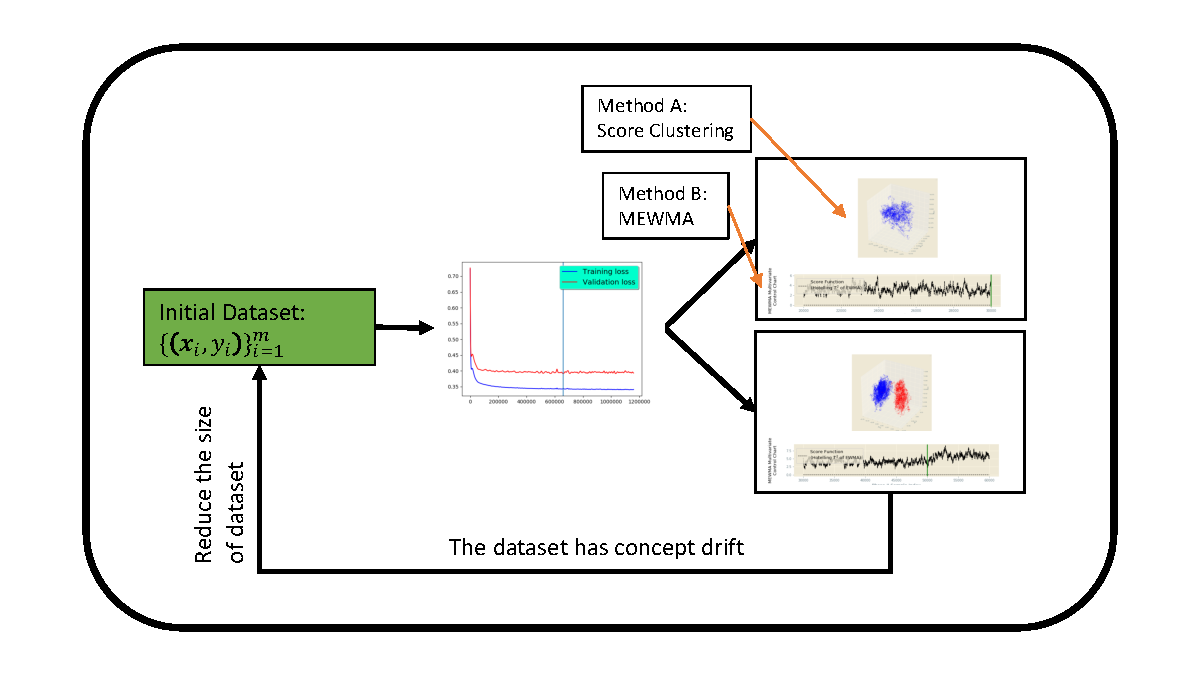
\includegraphics[width = 1\linewidth, trim=1.55in .85in 1.55in .85in, clip]{../figures/v14/flow_chart/Retrospective.png}
         \caption{Retrospective Analysis.}
         \label{fig:retro_analysis}
  \end{subfigure}
  \begin{subfigure}[t]{0.49\linewidth}
         \centering
         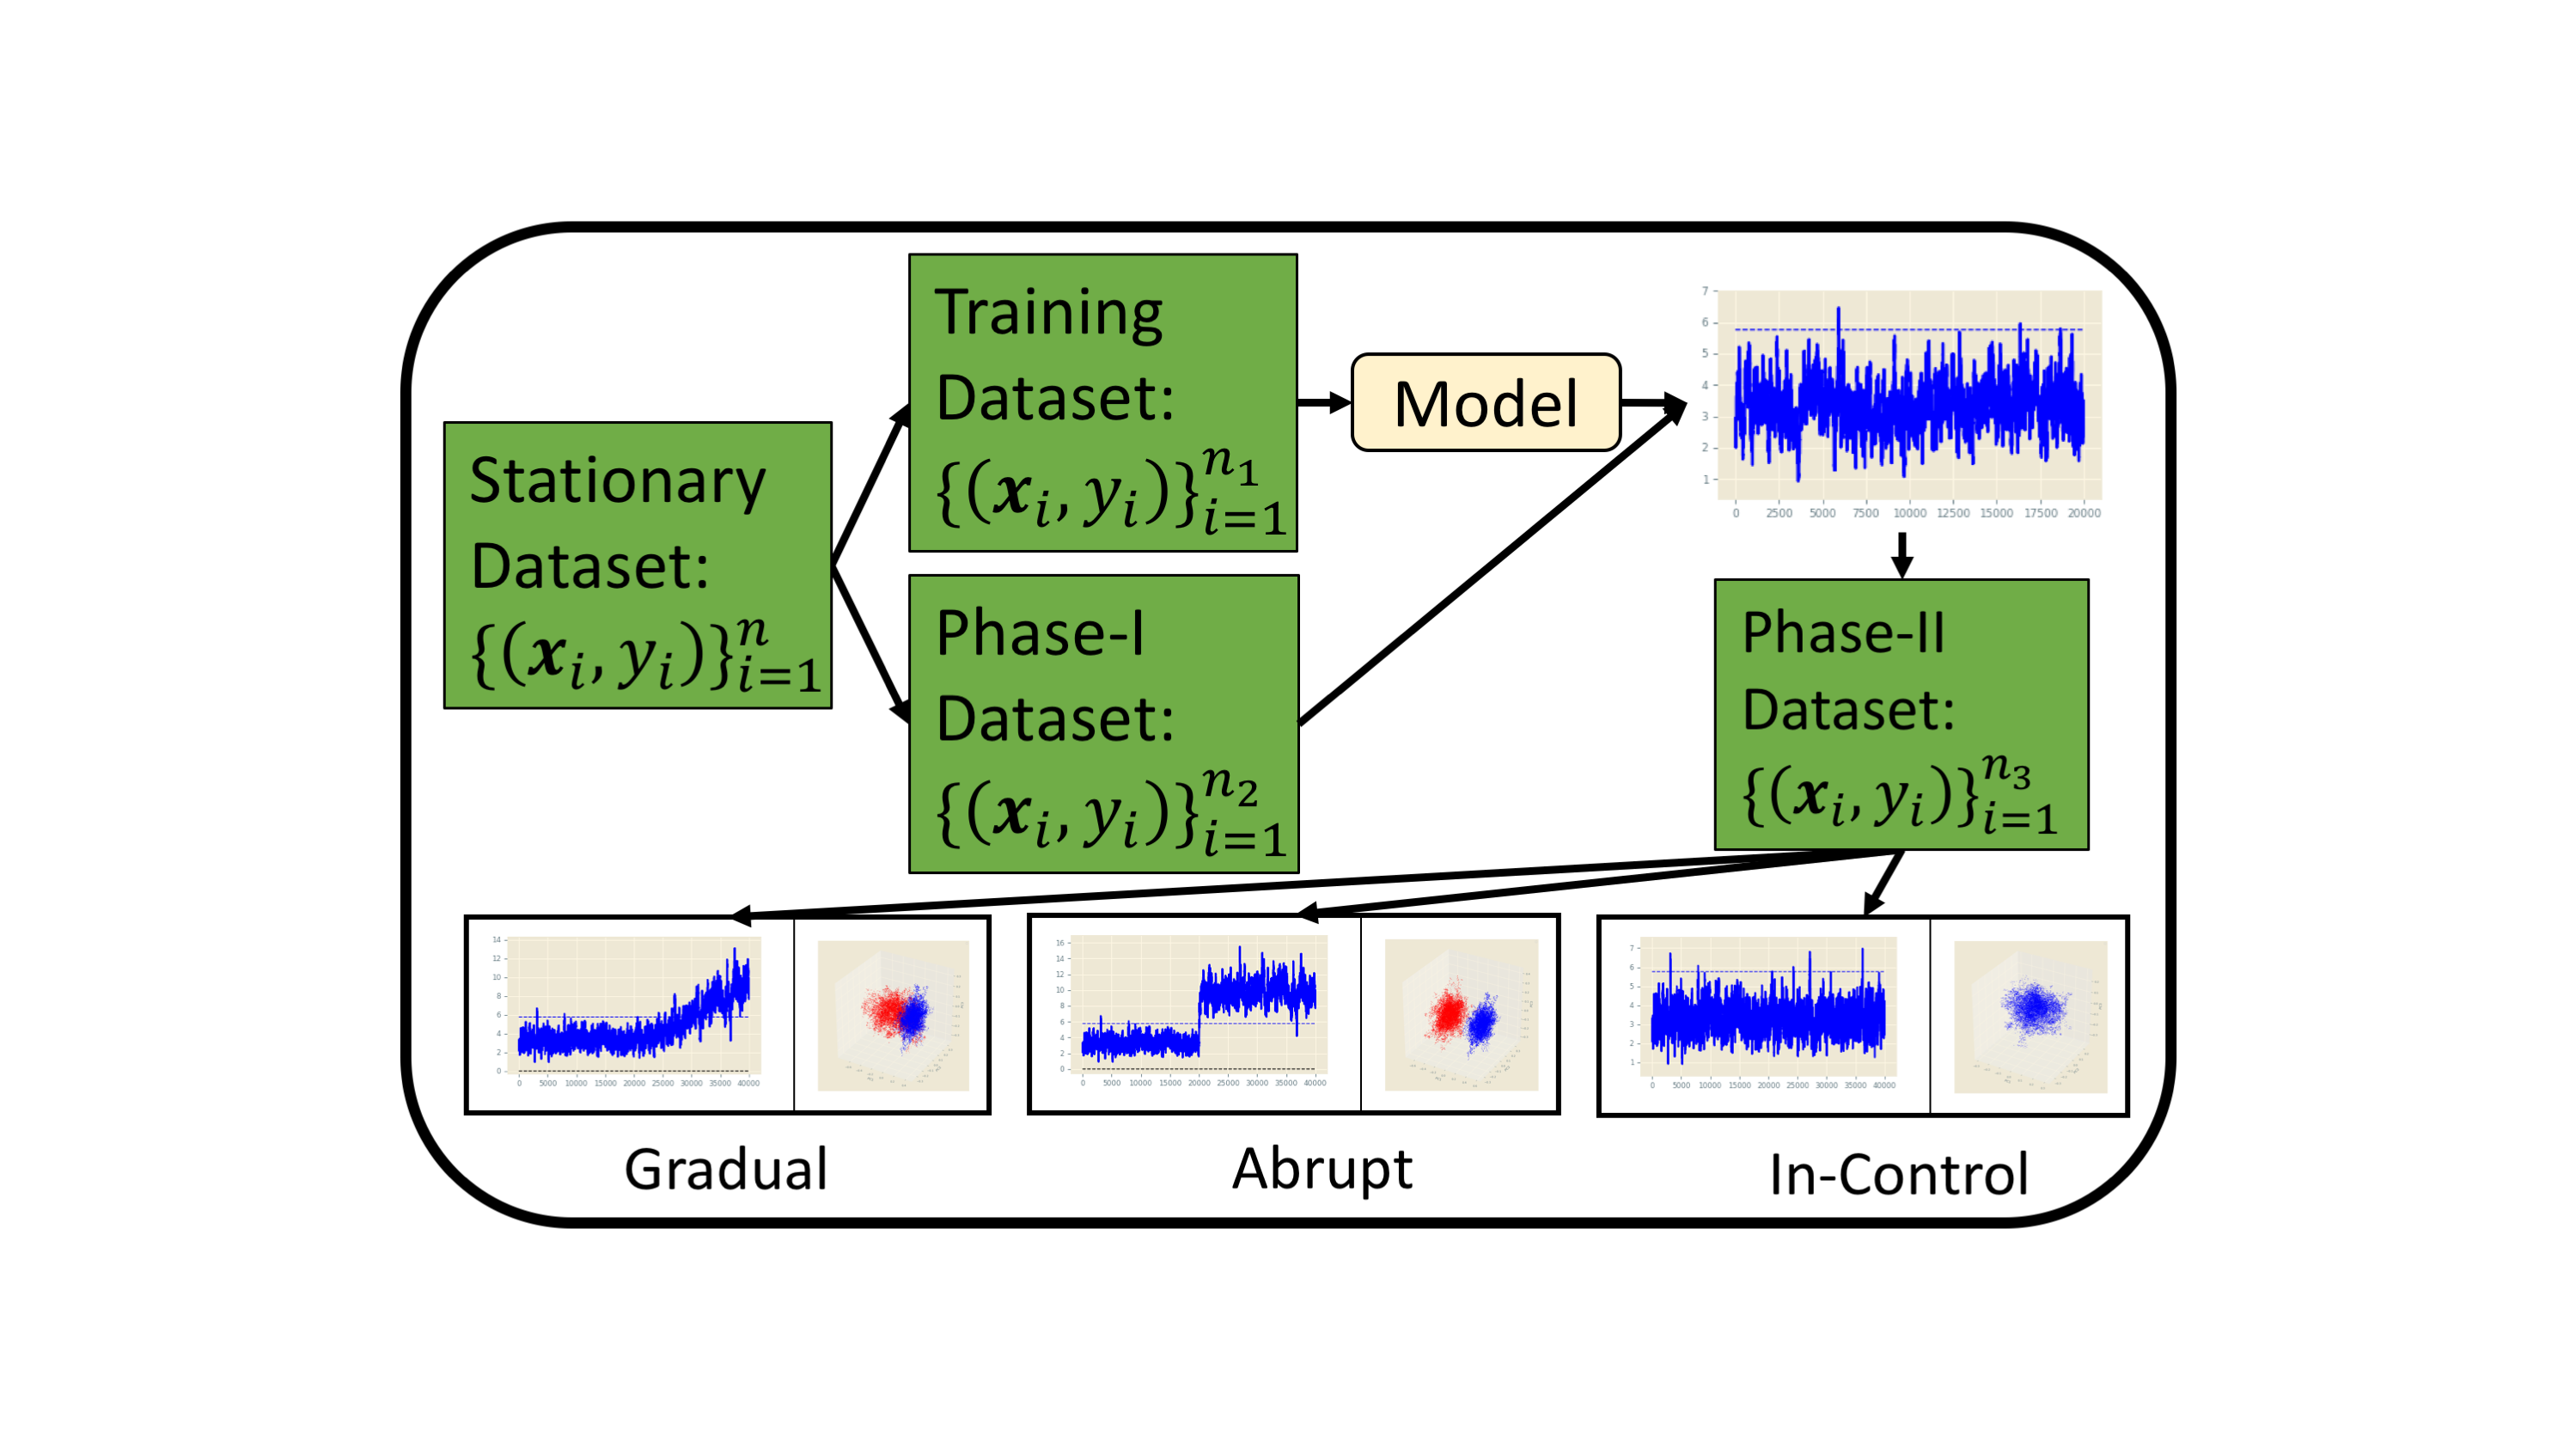
\includegraphics[width = 1\linewidth, trim=1.55in .85in 1.55in .85in, clip]{../figures/v14/flow_chart/Monitoring.png}
         \caption{Monitoring.}
         \label{fig:Monitoring}
  \end{subfigure}
  \begin{subfigure}[t]{0.49\linewidth}
         \centering
         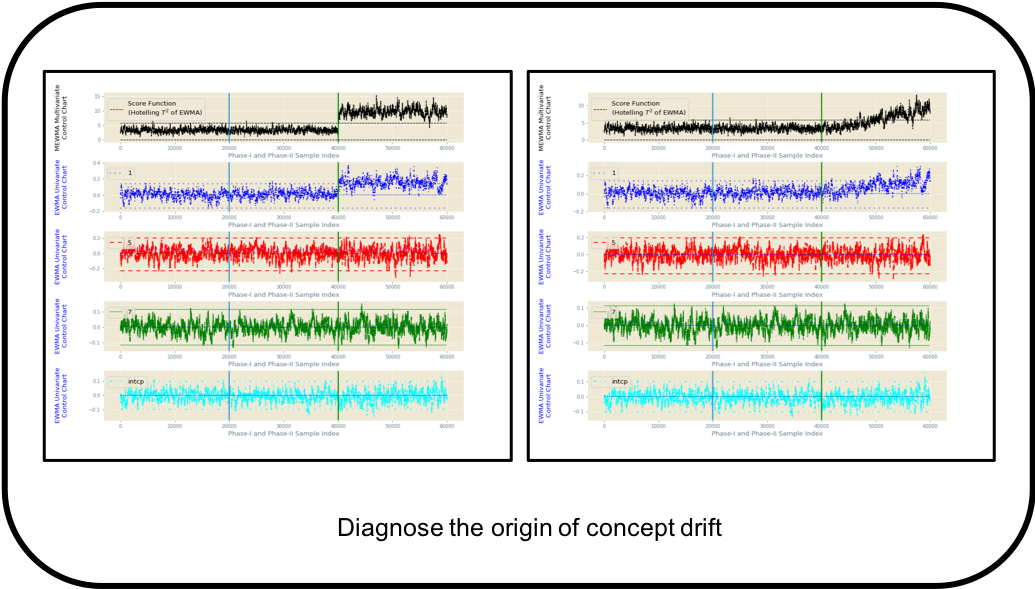
\includegraphics[width = 1\linewidth, trim=1.55in .85in 1.55in .85in, clip]{../figures/v14/flow_chart/Diagnose.png}
         \caption{Diagnosis.}
         \label{fig:diagnosis}
  \end{subfigure}
  \caption{{The framework of monitoring/detecting concept drift based on the score function. (a) Conducting retrospective analysis using MEWMA and/or score function clustering to ensure there is no concept drift in the data set used to train and set control limits. The size of data set can be recursively reduced if significant concept drift exists. (b) Monitoring concept drifts using the model and control limits obtained by processing training and Phase-I data sets, which will be demonstrated in Section~\ref{s:demon_cd} and~\ref{s:real_data}. In this subplot, three examples of possible results are given: gradual and abrupt concept drift and in-control case. (c) Visualization of diagnosing concept drift: The MEWMA for score vectors and the EWMA for individual predictors are visualized to show the origin of concept drift, which will be illustrated in Section~\ref{s:demon_cd} and~\ref{s:real_data}.}}
  \label{fig:proc_mon_score}
\end{figure}

% \subsubsection{Other Models}
% \begin{figure}[!htbp]
% \centering
%  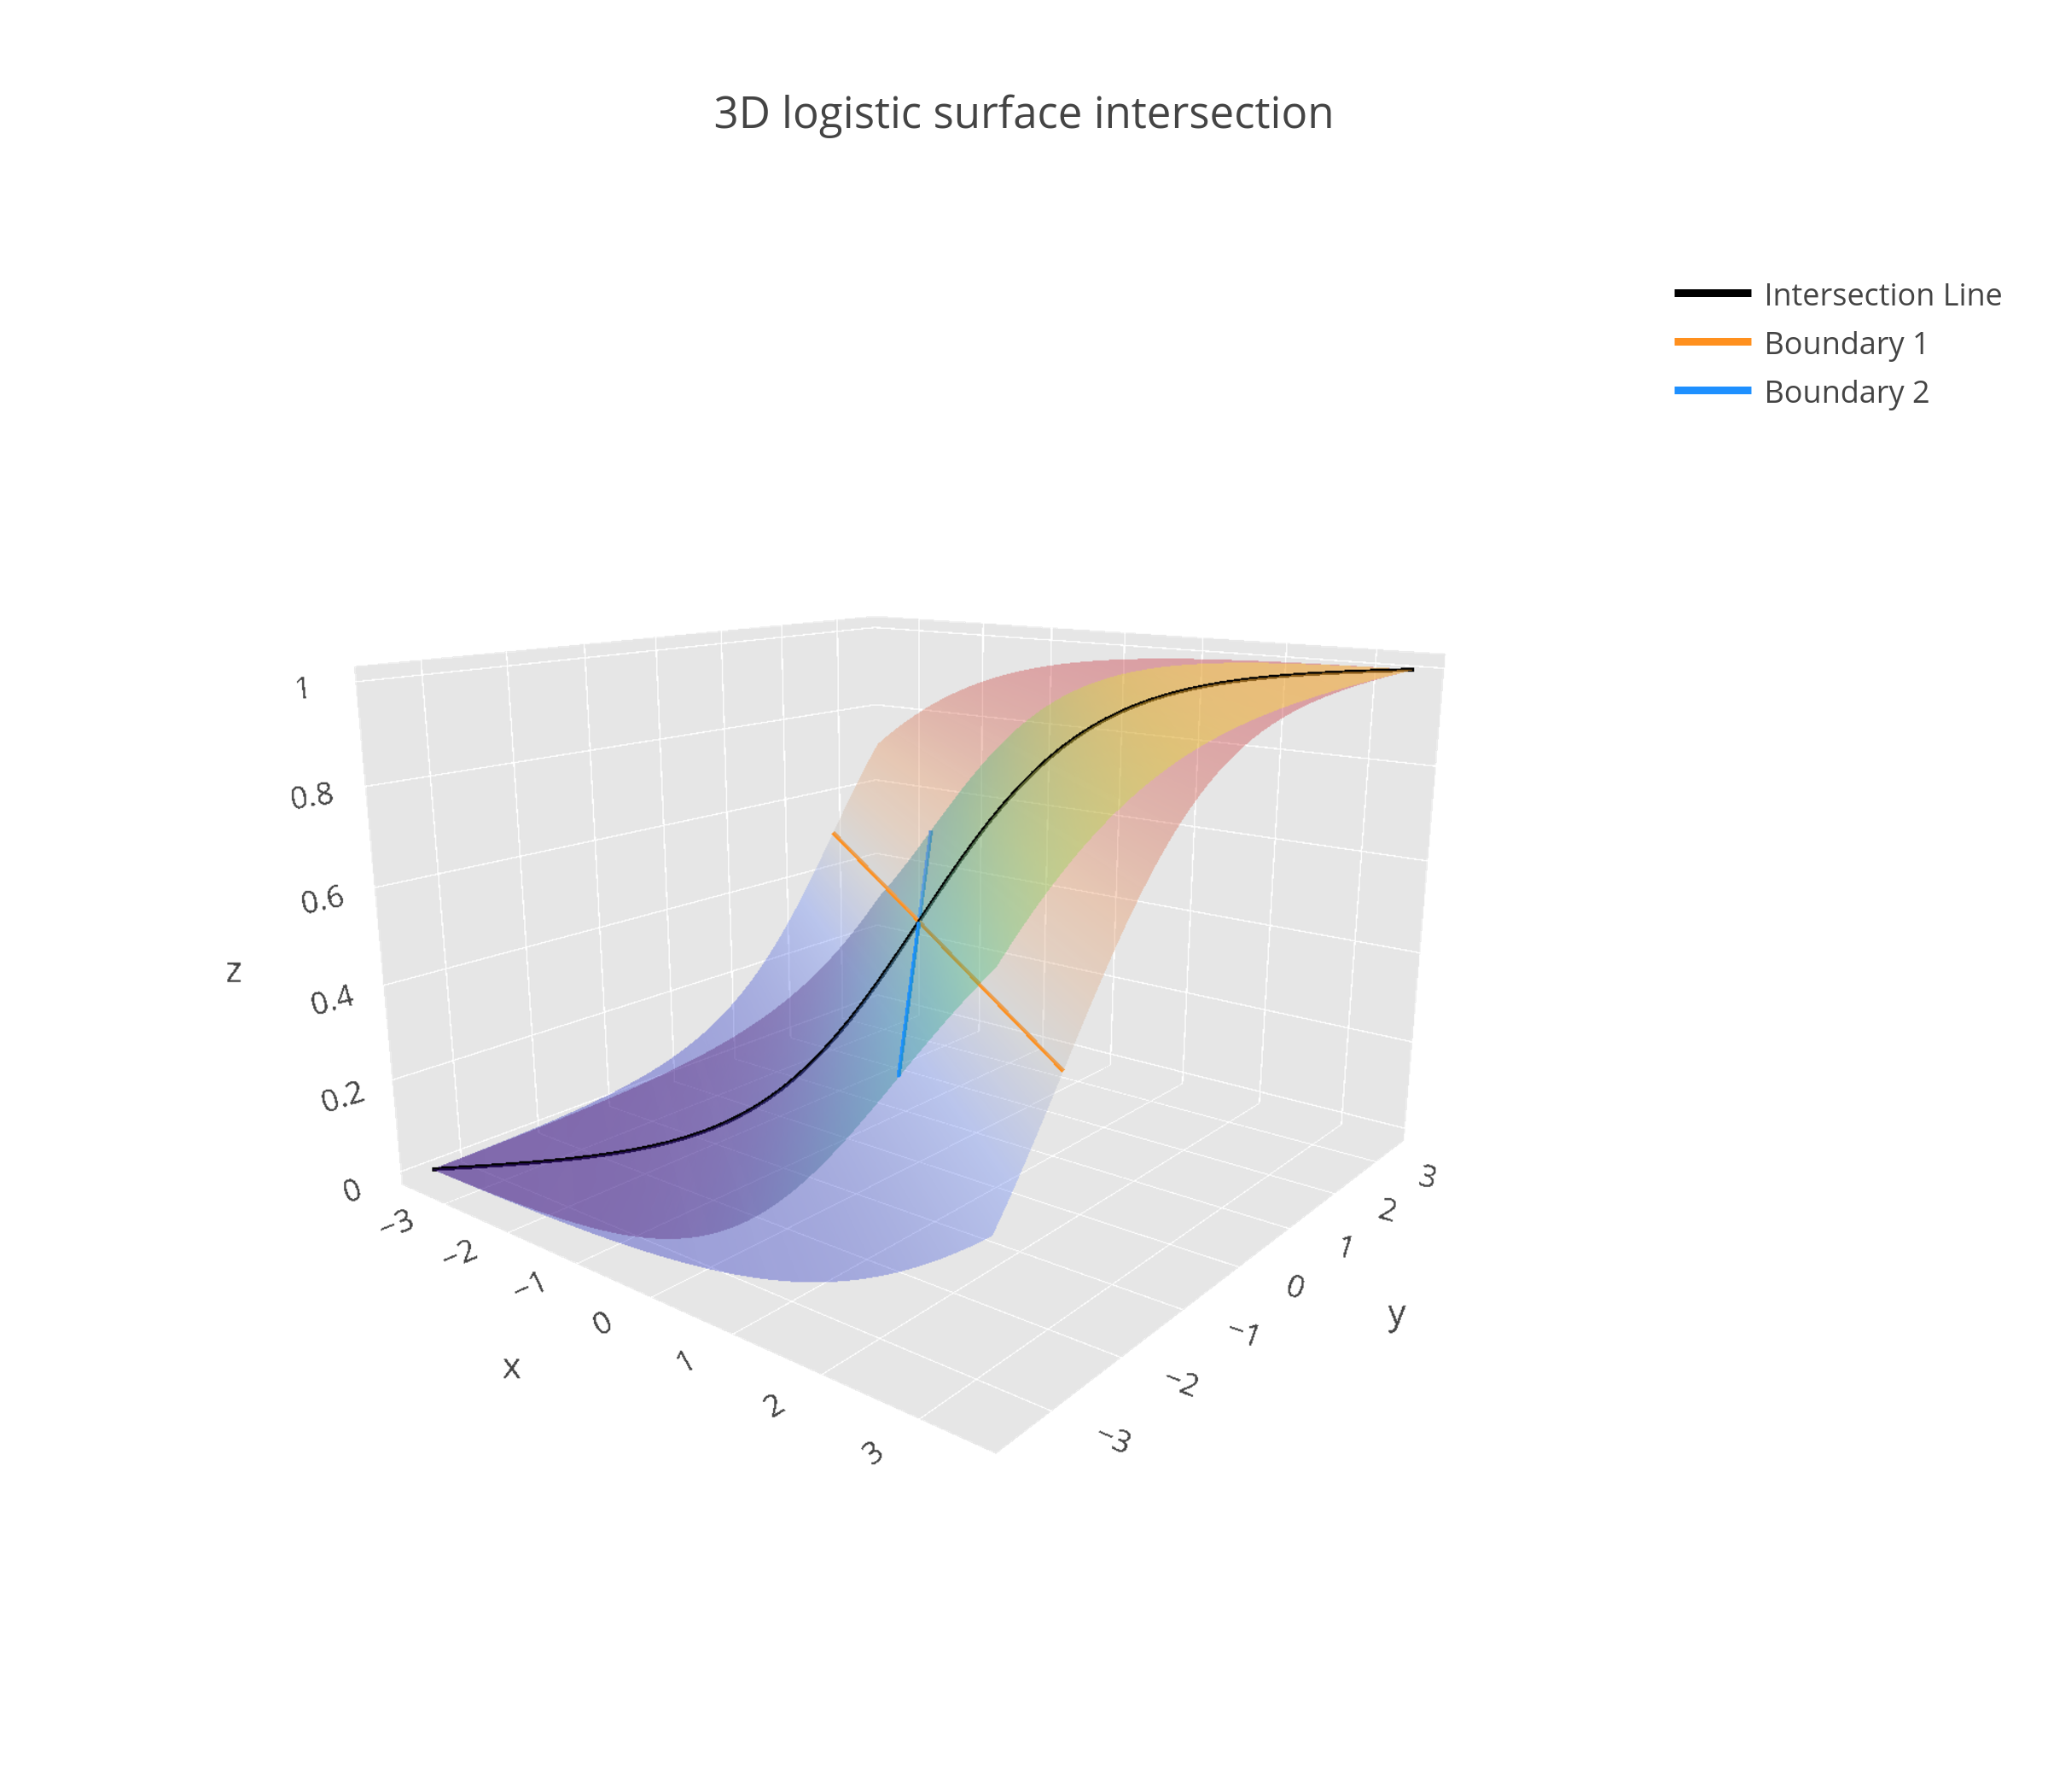
\includegraphics[width = 0.5\textwidth]{../figures/v14/demons_fig/3D_logistic_surface_intersection.png}
%   \caption{The demonstration of multiple logistic regression that concept drift would result in no change in expected error rate.}
%   \label{fig:logi_3d}
% \end{figure}
% The phenomenon observed in simple logistic regression can also be extended to multiple logistic regression. As shown in the Figure~\ref{fig:logi_3d}. Here, two logistic surfaces are plotted together, with the black line as the intersection and blue and orange lines are the optimal decision boundary for two models respectively. In this example, the error rate would not change with concept drift, because after concept drift the original model would increase local error rate in some region and decrease it in the other, resulting in zero net change in error rate. 

% Besides logistic regression for binary classification data, the score-based method can also be easily applied on multinomial classification. 

%Besides extended to the cases with higher dimension of predictor, the score-based methods can also be applied to classification problem with more than $2$ classes, while most of methods proposed are for binary classification problems.

% \subsubsection{Non-Zero Mean of Score Function with Concept Drift}
% \label{ss:non_zero_mean_score}


% How to formally define detection;
% How to quantify the relationship between the rate of detection and the rate of concept drift. Any power law?
% How to quantify the relationship between the rate of detection, the rate of concept drift, and the absolute value of concept drift. Any power law?
% After carefully define and quantify detection of concept drift in the simplest case, we can start to think about the online learning rate of more complex concept drift pattern. For example, when we have an alternative concept drift pattern. How should we choose statistics to monitor to get a better estimation of parameters in concept drift. In the online training context, early detection and change learning rate according maybe a way to solve concept drift problem better.

\subsection{Monitoring Sample Score Vectors with the High-Dimension Vector of Parameters}
\label{ss:high_dim_score}
One of the advancement of machine learning is that models become increasingly complex. Some models can have millions of parameters, like convolutional neural network. To monitor those models for concept drift, we can calculate sample score vectors when we make prediction or finely tune models. However, with such high-dimension of parameters, the inverse of the sample covariance matrix in the equation~(\ref{eqn:hotellingt2}), $\hat {\bm { \Sigma}}$, is very likely to be close to singular. For example, when the sample size of our training data (denoted as $N_1$ as in the Section~\ref{ss:imp_score_method}) is smaller than the dimension of parameters, $dim(\bm { \theta})$, the sample covariance would be singular. 

To solve this problem, we can add a nugget parameter on all diagonal entries of $\hat {\bm { \Sigma}}$ or use pseudo-inverse of the sample covariance. For the method of adding a nugget parameter $ \delta$, we assign $\hat {\bm { \Sigma}}+ \delta \bm {I}$ to $\tilde {\bm { \Sigma}}$ as the approximated covariance matrix. To understand the effect of this nugget parameter, denote the eigen-decomposition of the sample covariance matrix as $\hat {\bm { \Sigma}} = \bm {Q}\bm { \Lambda} \bm {Q}^T$ and obtain the eigen-values as $ diag(\bm{\Lambda}) = [ \lambda_1, \lambda_2,\cdots, \lambda_n]$ in a non-increasing order. Then, we can write the approximated sample covariance matrix as $\tilde {\bm { \Sigma}} = \bm {Q}\tilde{\bm { \Lambda}} \bm {Q}^T$, where $\tilde{\bm { \Lambda}} = \bm { \Lambda} + \delta \bm {I}$. The EWMA of the new statistics with this modified covariance matrix in the equation~(\ref{eqn:hotellingt2}) would not have the issue of ill-conditioning by suppressing unimportant directions of variation. 

Setting a condition number achieves a similar purpose. By setting a maximum condition number, $ \gamma$, we set all $ \lambda_i$ equal to $0$, if $ \lambda_1 \geq \gamma \lambda_i$. Denote the maximum of the index of $ \lambda_i$ which is not set to $0$ as $k$ and a new diagonal matrix $\bm { \Lambda} ^{-}$ with diagonal entries as $[1/\lambda_1,1/\lambda_2, \cdots, 1/\lambda_k, 0, \cdots, 0]$. Then, a pseudo-inverse of the sample covariance matrix is defined as $\hat {\bm { \Sigma}} ^{-} = \bm {Q}\bm { \Lambda}^{-}\bm {Q}^T$. This is equivalent to applying PCA onto $\bm {z}_t$, so that the most important variations in $\bm {z}_t$ are kept. 

Comparing with adding a nugget parameter, even though both methods give similar results, setting the maximum condition number is more intuitive in terms of controling the behavior of inverting the covariance matrix, while adding the nugget allows the concept drift to be detected in those directions, that would be otherwise set to $0$ in hard thresholding by setting the maximum condition number. So we choose to add a nugget parameter.

\subsection{Score function of Regularized Models}
\label{ss:score_regu}
In many current applications, models become increasingly complex, which almost always require regularization to combat overfitting. The regularization term is used to penalize complex models and large parameters, by minimizing negtive log-likelihood plus a norm of paramters, for example, $L_2$ norm of all parameters: $l(\bm{\theta})=-\frac{1}{n}\sum_{i=1}^n \ln P(y_i|\bm{x}_i;\bm{\theta})+\frac{c}{2}||\bm{\theta}||_2^2$, where $c>0$ is a regularization parameter. The regularization term would change the score function of the original model: $\nabla_{\bm{\theta}}l(\bm{\theta}) = -\frac{1}{n}\sum_{i=1}^n\bm{s}(\bm{\theta};(\bm{x}_i,y_i))+c\bm{\theta}$. It can be looked as a prior on parameters from Bayesian perspective, which can be ``distributed" among all data: $\nabla_{\bm{\theta}}l(\bm{\theta})=-\frac{1}{n}\sum_{i=1}^n(\bm{s}(\bm{\theta};(\bm{x}_i,y_i))-c\bm{\theta})=-\frac{1}{n}\nabla_{\bm{\theta}}\sum_{i=1}^n\ln(P(y_i|\bm{x}_i;\bm{\theta})\exp\{-\frac{c}{2}||\bm{\theta}||_{2}^2\})$. And treat the likelihood times prior as the new model: $P(Y|\bm{X};\bm{\theta})\exp\{-\frac{c}{2}||\bm{\theta}||_{2}^2\}$. Then, all methods of calculating score vectors and applying EWMA and Hotelling $T^2$ follows. In some popular form of penalization, this would not change the monitoring statistics. For example, adding a $L_2$ regularization term of all parameters would only add a constant vector to all score vectors: $\bm{s}(\bm{\theta};(\bm{x}_i,y_i))-c\bm{\theta}$. Adding regularization would have another good effect. When $dim ( \bm { \theta})$ is too large, $L_2$ penalization would add a diagonal matrix with positive entries to the sample covariance matrix: $-\nabla_{\bm{\theta}}(\bm{s}(\bm{\theta};(\bm{x}_i,y_i))-c\bm{\theta})=-\nabla_{\bm{\theta}}\bm{s}(\bm{\theta};(\bm{x}_i,y_i))+c\bm{I}=\mathbf{I}(\bm{\theta})+c\bm{I}$, where $\mathbf{I}$ and $\bm{I}$ are Fishier information and identity matrix respectively, automatically resulting in a well-conditioned matrix. We will encounter a regularization in neural network models. 

% Here another way is use pseudo-inverse.
\section{Decoupling of Concept Drift for Multivariate Regression and Classification}
\label{s:decou_cd}
While detecting the concept drift, we want to pinpoint which {covariates} have significant impact on the change of {the} conditional distribution {$P(Y| \bm {X}, \bm{\theta})$}. This can provide interpretability for concept drift for updating or fixing models. In some industry (e.g. financial, insurance, manufacturing), model interpretability is valued or even required by laws. Ideally, after decoupling, univariate control charts should truly reflect whether covariates have concept drifts or not. However, even for those covariates without concept drifts, the variance would increase due to variance of $\bm {X}$. More detailed analysis will follow in this section.

\subsection{Concept Drift Decoupling}
\label{ss:diagnosis}
To detect which covariates have concept drift, naively monitoring component-wise mean {drift} of the score function would fail when {covariates considerably correlate with each other} or nonlinear predictive models are used. To demonstrate this, look at linear model and logistic regression. Assuming the vector of the true parameters {before concept drift $\bm { \theta}^ { (0)}$} is known (we ignore the difference between the true parameter, $\bm { \theta}^ { (0)}$, and the estimator of it, $\hat{\bm { \theta}}$, as discussed in Section~\ref{ss:sgd_score}), the linear regression and the corresponding score function imply that {$E_{\bm{ \theta}^{ (0)}}[(Y - \bm {X}^T\bm { \theta}^{ (0)} ) \bm {X}|\bm {X}]=0$}. Note the notation that, the subscript, ${ \bm{\theta}}^{ (0)}$, of the expectation is the vector of parameters of the underlying distribution the expectation is taken with respect to, and the $\bm{ \theta}^{ (0)}$ in the expectation is the value taken for that vector. The two can be different, when the mean drift of concept drift is derived. After concept drift, {assuming the parameter $\bm { \theta}^{ (0)}$ changes to $\bm { \theta} ^{ (1)}$, denote the change in the vector of parameters as $ \Delta \bm { \theta} = \bm { \theta} ^{ (1)} - \bm { \theta}^ { (0)}$ for the rest context.} {The} joint expectation for the score function is $E [\bm {X}\bm {X}^T] \Delta \bm { \theta}$, where the concept drift only decouples when $E [\bm {X}\bm {X}^T]$ is a diagonal matrix, meaning all components of $\bm{X}$ are uncorrelated. For logistic regression, the joint expectation of the score function, $E[(\sigma ( \bm {  \bm {X}^T \theta}^{ (1)}) - \sigma ( \bm {X}^T\bm { \theta}^{ (0)} )) \bm {X}]$,  no longer has a clean format, because it depends on the unknown parameter vector, $\bm { \theta} ^{ (1)}$, after concept drift. In the next section, results from simulated data show that this mean {drift} is not decoupled even when $X _{i} (i = 1,2, \cdots, p)$ are uncorrelated. 

To decouple the interleaved drifts of parameters, for linear regression, we can simply pre-multiply sample score vectors by the {the inverse of the estimated} $E [\bm {X}\bm {X}^T]$, because this matrix does not depend on the actual drift in parameters (otherwise, it is generally hard to estimate when concept drift starts). However, this is not universally viable for more complex models, like in logistic regression. In general, the mean {drift} of the score function after concept drift is
\begin{align}
\begin{aligned}
E _{\bm { \theta}^{ (1)}}[\bm{s}(\bm { \theta}^{ (0)}; (\bm {X}, Y))] 
= & E[E _{\bm { \theta}^{ (1)}}[\bm{s}(\bm { \theta}^{ (0)}; (\bm {X}, Y))| \bm {X}] ] \\
= & E[\int _{y}\bm{s}(\bm { \theta}^{ (0)}; (\bm {X}, y)) P(y | \bm {X}, \bm{\theta} ^{ (1)}) dy ]
\end{aligned}
\label{eqn:cd_mean_shift}
\end{align}
Apply Taylor expansion on the $\bm{s}(\bm { \theta}^{ (0)}; (\bm {x}, y))$ around $\bm { \theta} ^{ (1)}$
\begin{align}
\begin{aligned}
 &\bm{s}(\bm { \theta}^{ (0)}; (\bm {x}, y)) = \bm{s}(\bm { \theta}^{ (1)}; (\bm {x}, y)) 
 + \nabla _{\bm { \theta}}{ \bm{s}(\bm { \theta}^{ (1)}; (\bm {x}, y))}(\bm { \theta}^ { (0)} - \bm { \theta} ^{ (1)}) 
 + o(\bm { \theta}^ { (0)} - \bm { \theta} ^{ (1)} ) 
\end{aligned}
\label{eqn:sc_ty_expa}
\end{align}
Substitute equation (\ref{eqn:sc_ty_expa}) into (\ref{eqn:cd_mean_shift}) and use the property of the score function for $\bm { \theta} ^{ (1)}$.
\begin{align}
\begin{aligned}
& E _{\bm { \theta}^{ (1)}}[\bm{s}(\bm { \theta}^{ (0)}; (\bm {X}, Y))] \\
= & E[\int _{y} \bm{s}(\bm { \theta}^{ (1)}; (\bm {X}, y))P (y| \bm {X}, \bm{\theta}^{ (1)}) d y ] \\ 
 +&  E[\int _{y} [  \nabla _{\bm { \theta}}{ \bm{s}(\bm { \theta}^{ (1)}; (\bm {x}, y))}(\bm { \theta}^ { (0)} - \bm { \theta} ^{ (1)}) \\ 
 +& o(\bm { \theta}^ { (0)} - \bm { \theta} ^{ (1)} ) ] P (y| \bm {X}, \bm{\theta}^{ (1)}) d y]\\ 
= & E[E _{\bm { \theta}^{ (1)}}[\bm{s}(\bm { \theta}^{ (1)}; (\bm {X}, Y))| \bm {X}]] \\
+ & E[\int _{y} [ \nabla_{\bm { \theta}} \nabla^T _{\bm { \theta}}{ \ln f(\bm { \theta}^{ (1)}| (\bm {x}, y))}(\bm { \theta}^ { (0)} - \bm { \theta} ^{ (1)}) \\
+ & o(\bm { \theta}^ { (0)}- \bm { \theta}^{ (1)})]P (y| \bm {X}, \bm{\theta}^{ (1)}) dy] \\
= & \bm{0} +  \{E[E _{\bm { \theta}^{ (1)}}[\nabla_{\bm { \theta}} \nabla ^T_{\bm { \theta}}{ \log{f}(\bm { \theta}^{ (1)}| (\bm {x}, y))} | \bm {X}]] \\ + &o(1)\}(\bm { \theta}^{ (1)} - \bm { \theta}^ { (0)}) \\
= & [{\mathbf {I}}(\bm { \theta}^{ (1)})+ o(1)](\bm { \theta}^{ (1)} - \bm { \theta}^ { (0)}) \\
= & [{\mathbf {I}}(\bm { \theta}^{ (0)})+ o(1)](\bm { \theta}^{ (1)} - \bm { \theta}^ { (0)}) \\
%= & (\bm { \theta}^ {tr} - \bm { \theta}^{dr}) \int \left.\frac{\partial^2 \ln f (y | \bm {x}, \bm{\theta})}{\partial \bm { \theta}\partial \bm { \theta}^T}\right| _{\bm { \theta} = \bm { \theta}^{'}} f (y | \bm {x}, \bm{\theta}^{'}) d y \\
%+ & o(\bm { \theta}^* - \bm { \theta}^{'})  \\
%= & {\mathbf {I}}(\bm { \theta}^{'}|\bm {x})(\bm { \theta}^{'} - \bm { \theta}^*) + o(\bm { \theta}^* - \bm { \theta}^{'})  \\
%= & {\mathbf {I}}(\bm { \theta}|\bm {x})(\bm { \theta}^{'} - \bm { \theta}^*) + o(\bm { \theta}^* - \bm { \theta}^{'})
\end{aligned}
\label{eqn:cd_decomp_fisher_approx}
\end{align}
where {${\mathbf {I}}(\bm { \theta}^{ (0)})=E[E _{\bm { \theta}^{ (0)}}[\nabla_{\bm { \theta}} \nabla^T _{\bm { \theta}}{ \log{f}(\bm { \theta}^{ (0)}; (\bm {x}, y))} | \bm {X}]]$} is the (expected) Fisher Information Matrix {at parameter $\bm { \theta} ^{ (0)}$} and $o(\cdot)$ represents asymptotically negligible quantity comparing with the argument. Here, we use the fact that the expectation of the score function is $\bm {0}$ when {$\bm { \theta}^{ (1)}$} is true and assume {$ \bm { \theta}^ { (1)} - \bm { \theta}^{ (0)} $} small. To approximately decouple concept drift, we can pre-multiply sample score vectors by {the} inverse of {the} estimated {${\mathbf {I}}(\bm { \theta}^{ (0)})$}, or the sample covariance matrix of {the score function.}

\subsection{Variance Inflation for Covariates without Concept Drift}
\label{ss:var_infla}
{Notice that the expectation in~(\ref{eqn:score_exp_zero}) is with respect to the conditional distribution, but the sample score vector, {$\bm{s} (\bm { \theta} ^{ (0)};(\bm {x}_i, y_i))$}, has randomness from not only $P_{\bm {\theta}} (Y|\bm {X};\bm{\theta}^{(0)})$ (where $\bm { \theta} = \bm { \theta}^{(0)}$ when no concept drift) but also $P (\bm {X})$. In other words, monitoring mean {drift} of {$\bm{s} (\bm { \theta}^{ (0)};(\bm {x}_i, y_i))$} using control charts (which will be formally introduced later) is practically implemented by monitoring drift of {$E _{ \bm { \theta}}[\bm{s} (\bm { \theta}^{ (0)};(\bm {X}, Y))]$}.
%\begin{align}
%\begin{aligned}
%&E _{\bm { \theta}^{tr}}[\bm{s}(\bm { \theta}^{tr}| (\bm {X}, Y))| \bm {X}=\bm {x}] \\
%= & \int _{y}\bm{s}(\bm { \theta}^{tr}| (\bm {x}, y)) p(y | \bm {x}, \bm{\theta} ^{tr}) dy\\
%= & \int _{y}\bm{s}(\bm { \theta}^{tr}| (\bm {x}, y)) f(\bm{\theta}^{tr}| (\bm {x},y)) dy = \bm {0}
%\end{aligned}
%\label{eqn:expe_score}
%\end{align}
To understand the relation, using iterative expectation, we have}
\begin{align}
E_{ \bm { \theta} }[\bm{s} (\bm { \theta} ^{ (0)};(\bm {X}, Y))] = E [E _{ \bm { \theta} }[\bm{s} (\bm { \theta} ^{ (0)};(\bm {X}, Y))|\bm {X}]]
\label{eqn:joint_expe}
\end{align}
{According to the definition, a concept drift corresponds to change in $E _{ \bm { \theta} }[\bm{s} (\bm { \theta} ^{ (0)};(\bm {X}, Y))| \bm {X}]$ from $\bm{0}$, because this indicates the change in $P(Y|\bm {X};\bm{\theta})$. In practice, we can not directly monitor $E _{ \bm { \theta} }[\bm{s} (\bm { \theta} ^{ (0)};(\bm {X}, Y))| \bm {X}]$, because of lack of control in randomness from $\bm {X}$. Instead, we actually monitor $E_{ \bm { \theta} }[\bm{s} (\bm { \theta} ^{ (0)};(\bm {X}, Y))]$. This actually makes sense, because the {drift} of the left-hand-side in the equation~(\ref{eqn:joint_expe}) implies the {drift} of inner expectation of the right-hand-side, meaning concept drift; the reverse is generally true except that {$E _{ \bm { \theta} }[\bm{s} (\bm { \theta} ^{ (0)};(\bm {X}, Y))| \bm {X}]$} has a specific form and non-zero values at different realizations of $\bm {X}$ cancel out after taking expectation with respect to $\bm {X}$. As shown in Section~\ref{ss:score_func}, under assumption of small changes and smooth conditions with respect to the parameter, for generalized linear model, concept drift in parametric models implies non-zero mean of score function.}

As mentioned before, the univariate score function corresponding to those covariates without concept drifts will have $\bm{0}$ mean in univariate control charts, but the variance would be inflated if concept drifts exist in other covariates so that the monitored statistics will still fall outside of control limits. Because of the clear pattern without mean drifts, these components should not be included as candidates of origins of concept drifts, and after recovering those covariates from concept drifts as required by some applications, the inflated variance in control charts should go back to normal. To give an example here, linear regression is used to show the origin of variance inflation.

For a linear regression mode, assuming that the data generation model after training phase is $y' = \bm {x}^T\bm { \theta}^{ (1)} + \epsilon$, the variance of the $k$th component of the score function after the concept drift is
%\begin{align}
%\begin{aligned}
%&Var _{\bm{ \theta}^{(0)}}[ (Y- \bm {X}^T\bm{ \theta}^{(0)}) X_{k}]  \\
%= & E _{ \bm{ \theta}^{(0)}} [(Y-   \bm {X}^T\bm{ \theta}^{(0)})^2 X_{k}^2] - E _{ \bm{ \theta}^{(0)}}^2 [(Y- \bm {X}^T\bm{ \theta}^{(0)} ) X_{k}]  \\
%= & E _{\bm{ \theta}^{(0)}} [(Y - \bm {X}^T\bm{ \theta}^{(0)})^2 X_{k}^2]  \\
%= & E [E _{\bm{ \theta}^{(0)}}[(Y - \bm {X}^T\bm{ \theta}^{(0)} )^2| \bm {X}] X_{k}^2]  \\
%= & \sigma^2 E[  X_{k}^2] = \sigma^2 \sigma_{x,k}^2
%\end{aligned}
%\label{eqn:var_bef_cd}
%\end{align}
\begin{align}
\begin{aligned}
&Var _{ \bm{ \theta}^{(1)}}[ (Y'- \bm {X}^T \bm{\theta}^{(0)}  ) X_{k}]   \\
%= & E  [Var  _{ \bm{ \theta}^{(1)}}[(Y' - \mu ) X_{k}]] + Var  [E  _{ \bm{ \theta}^{(1)}}[(Y' - \mu ) X_{k}]]   \\
%= & 
= & E _{\bm{ \theta}^{(1)}} [(\bm {X}^T \bm{\theta}^{(1)}+\epsilon -  \bm {X}^T \bm{\theta}^{(0)}  )^2 X_{k}^2] - E _{\bm{ \theta}^{(1)}}^2 [(\bm {X}^T \bm{\theta}^{(1)}+\epsilon - \bm {X}^T \bm{\theta}^{(0)}) X_{k}]   \\
= & E   [E _{\bm{ \theta}^{(1)}}[(\bm {X}^T\Delta \bm { \theta}  +\epsilon)^2|\bm {X}] X_{k}^2] - \Delta \bm{\theta}^T E   [\bm {X}  X_{k}]E   [\bm {X} ^T X_{k}] \Delta \bm { \theta}    \\
= & E   [ (\Delta \bm { \theta}^T \bm {X} \bm {X} ^T \Delta \bm { \theta} + \sigma^2)X_{k}^2] - \Delta \bm{\theta}^T E   [\bm {X}  X_{k}]E   [\bm {X} ^T X_{k}] \Delta \bm { \theta}    \\
= & \sigma^2 \sigma_{x,k}^2 + \Delta \bm{\theta}^TVar [\bm {X}  X_{k}] \Delta \bm{\theta}
\end{aligned}
\label{eqn:var_aft_cd}
\end{align}
where $ \sigma$ is the variance of random noise and $ \sigma _{x,k}$ is the variance of the $k$th component of the covariate. Clearly, $\Delta \bm{\theta}^TVar [\bm {X}  X_{k}]\Delta \bm{\theta}$ is generally non-zero if $ \Delta \bm { \theta} \neq \bm {0}$, resulting in variance inflation for predictor without concept drift. Notice that because the variance of lines in control charts depends on the covariate, ``covariate drift" (meaning change in distribution of $\bm {X}$) will also affect the variance in the control charts, but not mean. In this study, we assume no covariate drift.

\section{Demonstration of Monitoring the Score Function}
\label{s:demon_cd}
The concept drift in real data sets is notoriously hard to testify unless there is some strong posterior knowledge on when drifts happened. To test the properties mentioned in Section ~\ref{s:theory_analysis_score} and~\ref{s:decou_cd}, we first use simulated data sets. Here, we focus on simple but commonly used models like linear model, logistic regression, multinomial regression, poisson regression, and MLP, for the simplicity of proof-of-concept and analytical explanation. We expect that those properties can be extended to more complex models, because our previous analyses on the score function are mostly model and distribution agnostic. 

In the following demonstration and analysis, several experiments are shown the efficacy and properties of score-based method and its superior performance comparing with other metrics. First in Section~\ref{ss:cd_no_err_change}, simulations shown that concept drift can result in no change in expected error rate (thus no detection) on control charts, but large mean drift in score function. Then in Section~\ref{ss:simu_MRL}, Monte Carlo simulation experiments are conducted to calculate Median Run Length ($MRL$) for both in-control and out-of-control regions, showing that the score-based method has higher sensitivity in detection. At the last in Section~\ref{ss:cd_diag}, data sets with partially correlated covariates are simulated to show that the score-based method can decouple the concept drift, with proper transformation. Within this section, multiple kinds of data sets are simulated to demonstrate challenges in decoupling concept drifts in regression and classification and how our score-based method can handle them. 
%The generated data sets have independent or correlated covariates to illustrate the effect of decoupling operations and under which conditions they can be useful. Because the most of real data sets have more or less multi-collinearity, more emphasis is put on data sets having correlated covariates.
We also simulate abrupt and gradual concept drifts to test the performance of detecting and tracking concept drifts by monitoring the score function, as well as other metrics like EWMA of the prediction error or absolute residual. Those results show that monitoring the score function is a better and more versatile method in dealing with concept drift problems. 

\subsection{Concept Drifts with No Error Rate Change}
\label{ss:cd_no_err_change}
\begin{figure}[!htp]
\centering
\begin{subfigure}[t]{0.49\linewidth}
         \centering
        %   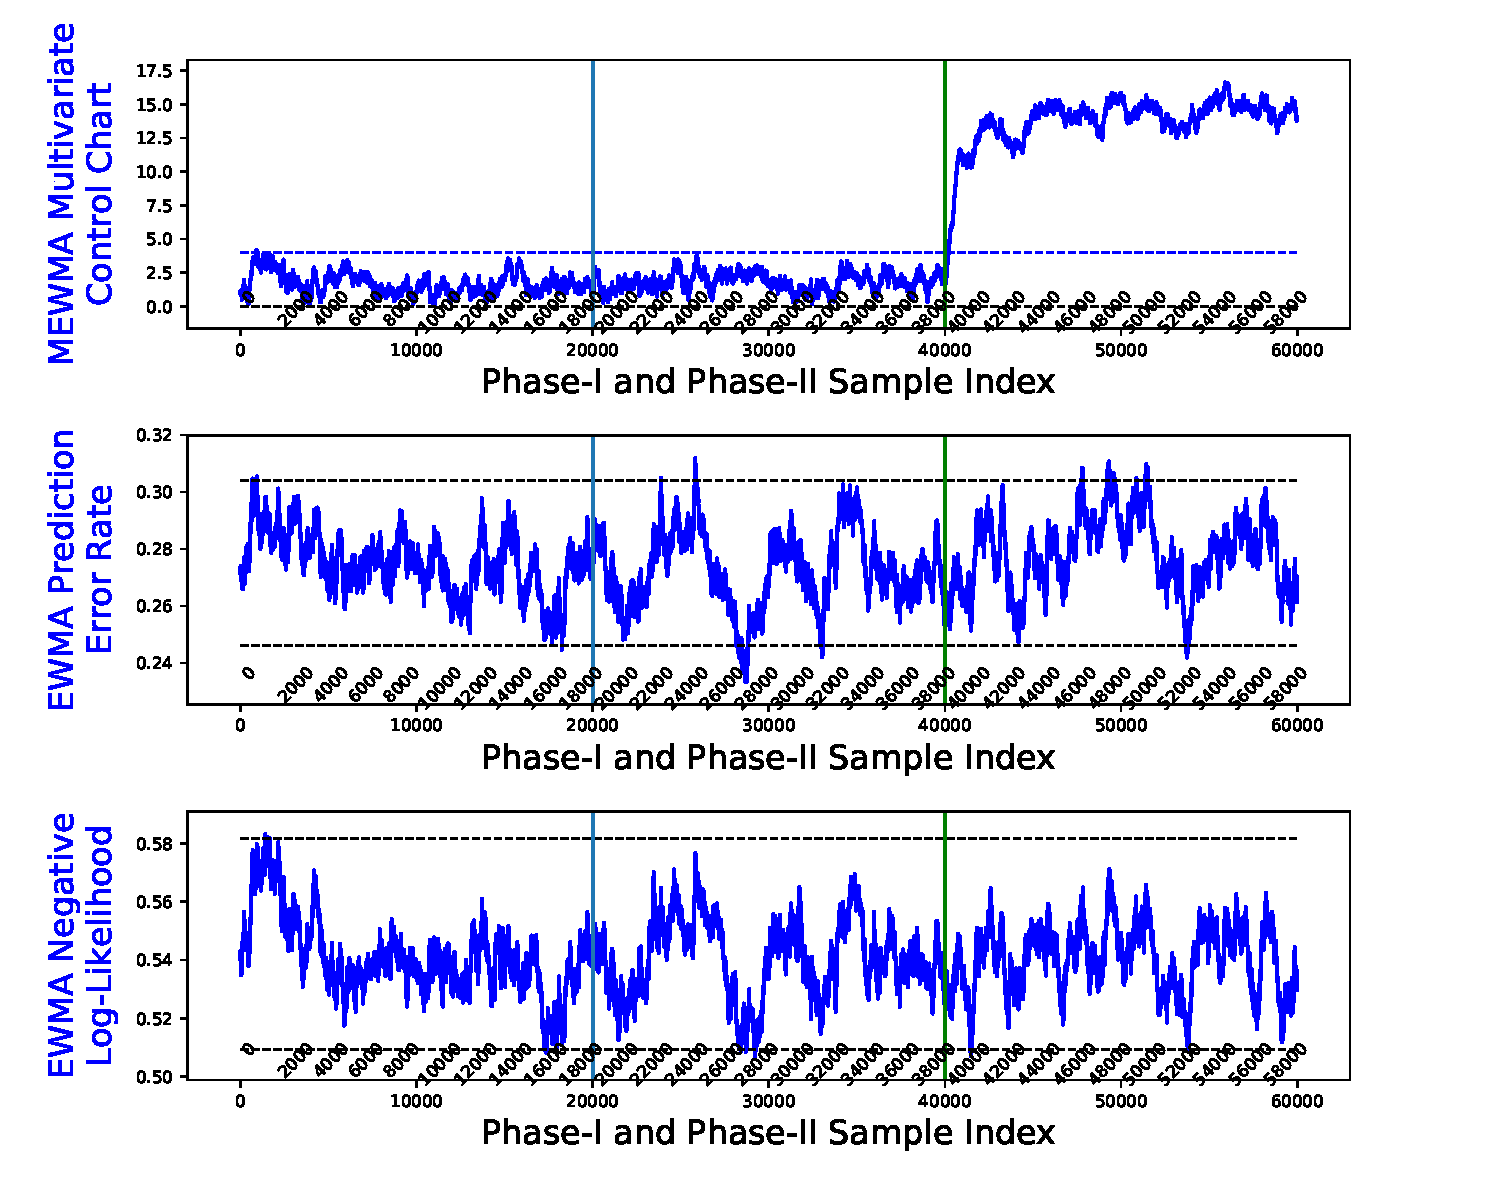
\includegraphics[width = \linewidth, trim=0in 2.6in 0in 0in, clip]{../figures/v14/sim_11/non_nnet_unif_ch_f_trans/1_sim11_logi_1e-08_0_0015_1.png}
           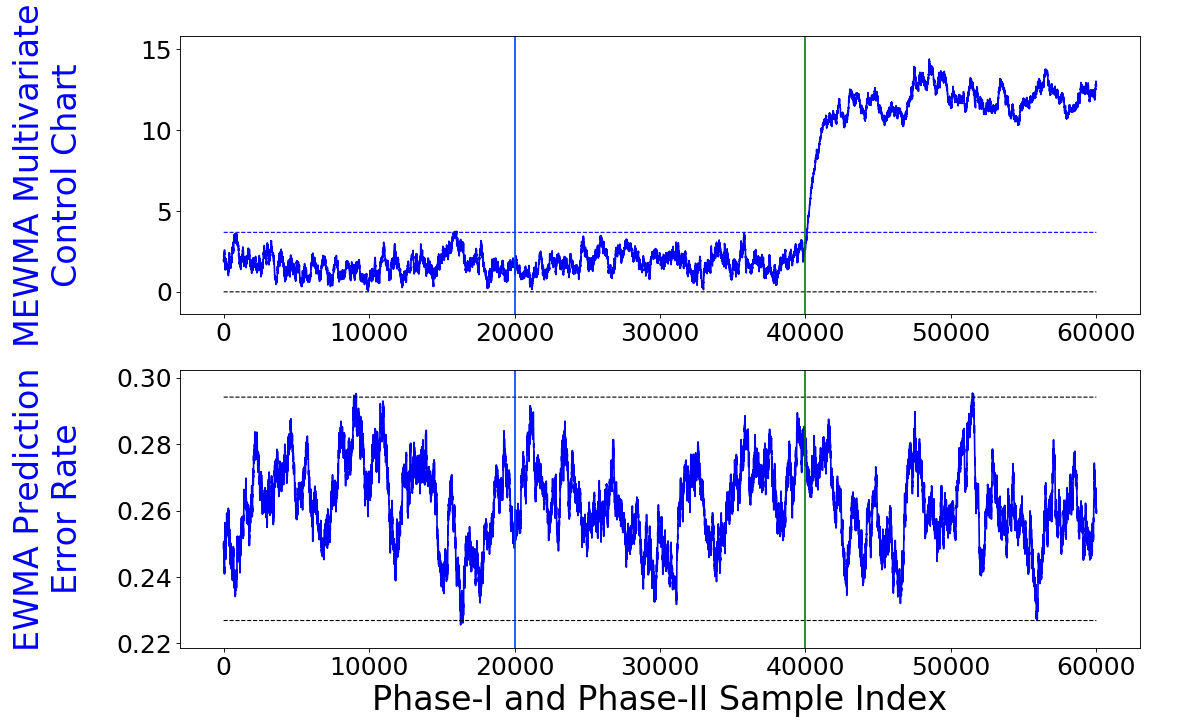
\includegraphics[width = \linewidth]{../figures/v14/sim_11/non_nnet_nonunif_ch_f_0_2/1_sim11_logi_1e-08_0_0015_1.png}
         \caption{Concept drift results in mean change in score-based method but no mean change in error rate.}
         \label{fig:exp_no_err_ch_a}
  \end{subfigure}
\begin{subfigure}[t]{0.49\linewidth}
         \centering
	       %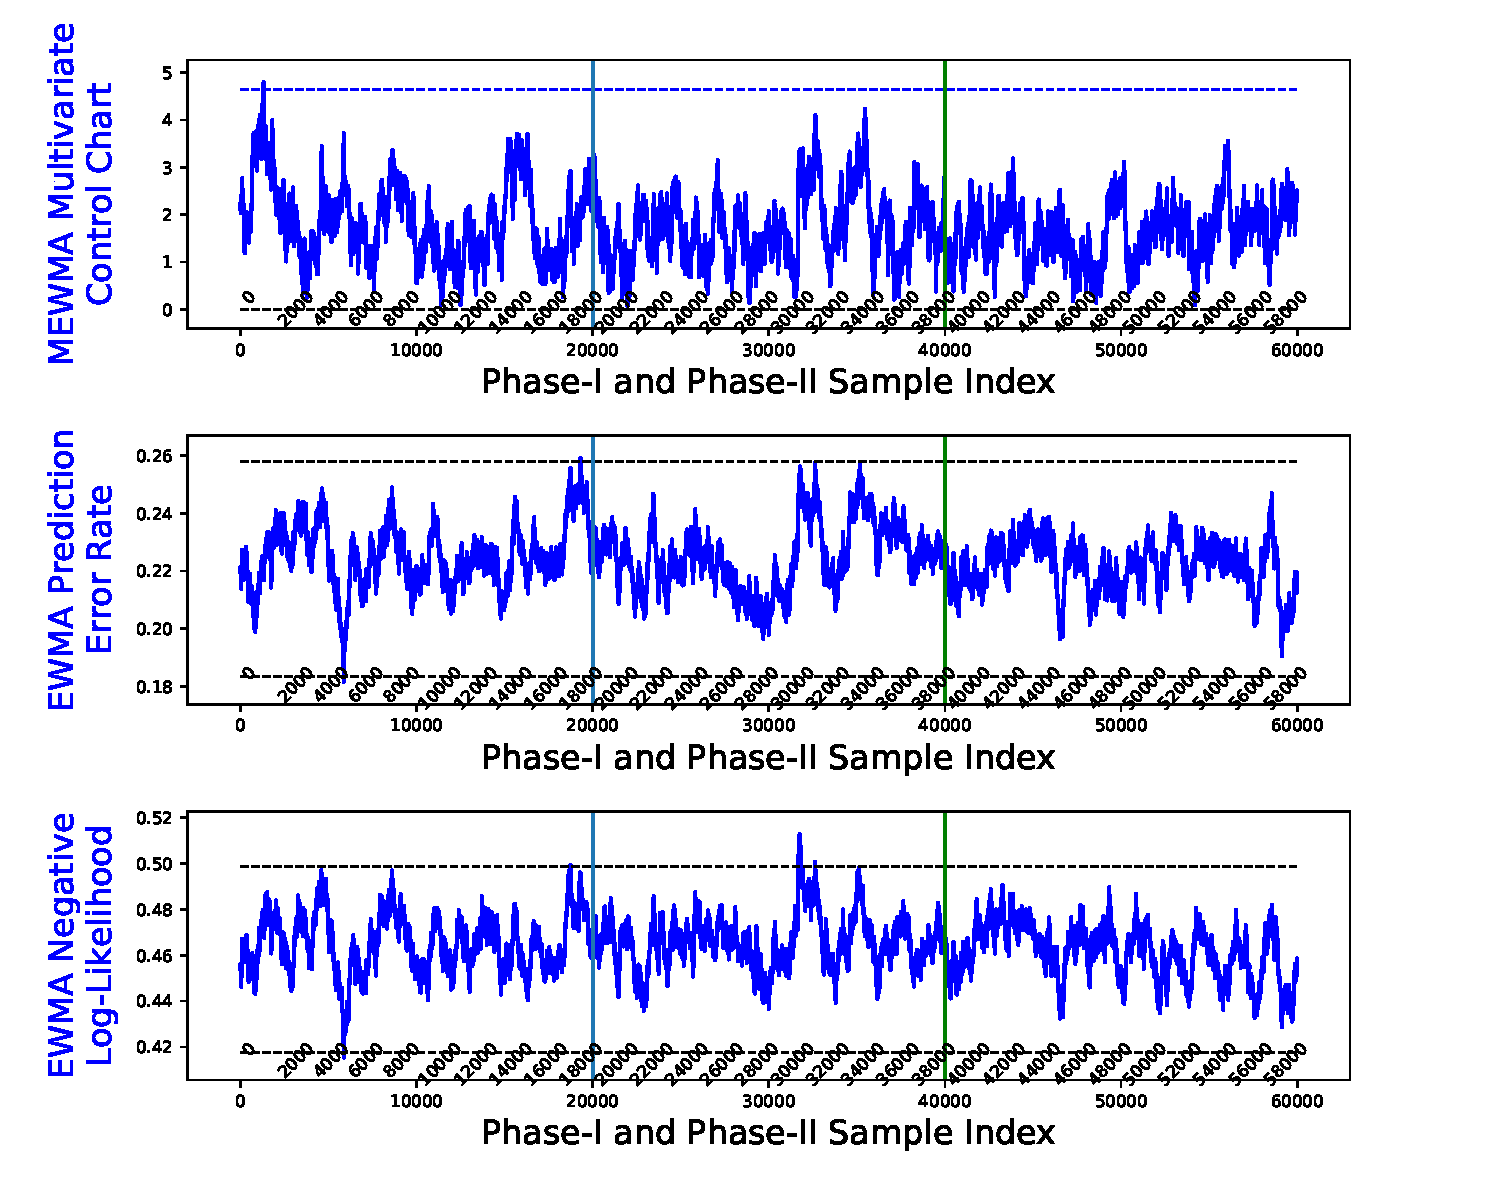
\includegraphics[width = \linewidth, trim=0in 2.6in 0in 0in, clip]{../figures/v14/sim_11/non_nnet_unif_ch_f_trans_followup/1_sim11_logi_1e-08_0_0015_1.png}
	       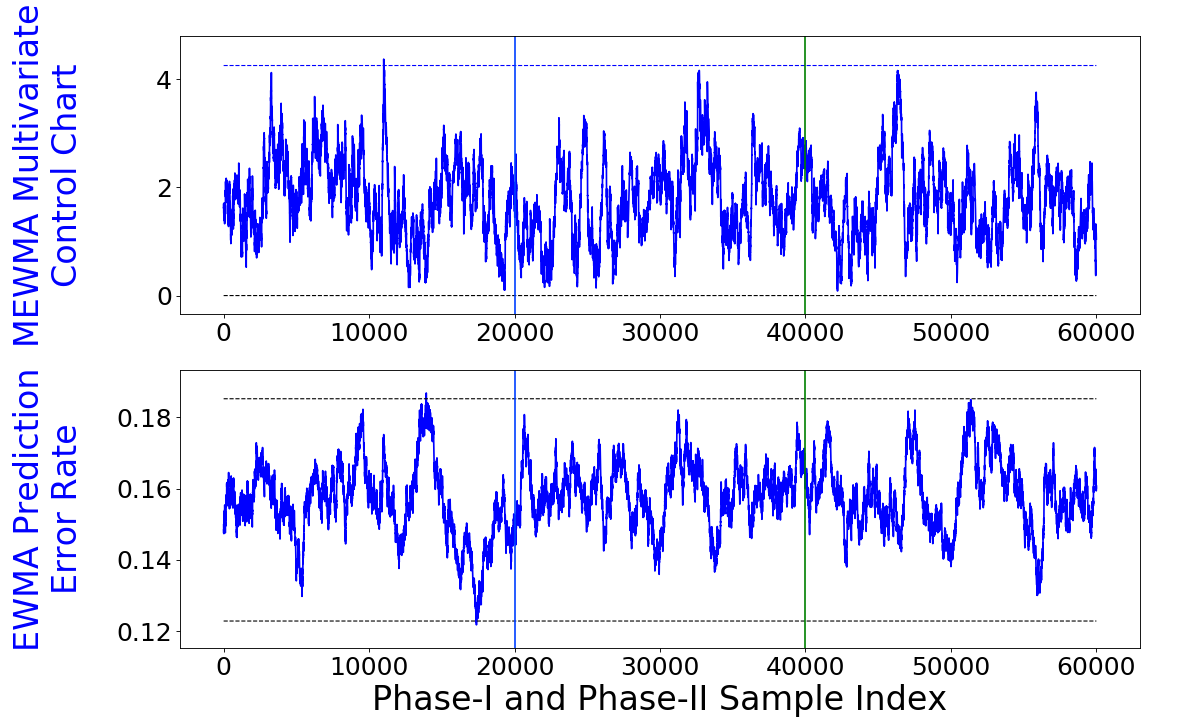
\includegraphics[width = \linewidth]{../figures/v14/sim_11/non_nnet_nonunif_ch_f_0_2_followup/1_sim11_logi_1e-08_0_0015_1.png}
         \caption{After retraining on the drifted data set, the performance of model increased, according to the lower control limit in prediction error.}
         \label{fig:exp_no_err_ch_b}
  \end{subfigure}
%  \includegraphics[width = 0.8\linewidth]{../figures/sim_2_pinv_pdf/sim2_ewma_2_metric_with_reg_1e-08_0_005.png}
%  \includegraphics[width = 0.48\linewidth]{../figures/sim_2_pinv/sim2_ewma_log_lik_with_reg_1e-08_0_005.png}
  \caption{A logistic regression example with two covariates, where before blue vertical line is Phase-I and the green vertical line is the boundary between before and after concept drift in the Phase-II. This example shows that our score-based method can detect concept drift which has no change in error. This detection provides an opportunity for improvement as shown in the lower limits on the right plots.}
  \label{fig:exp_no_err_ch}
\end{figure}
In Section~\ref{ss:imp_score_method}, simple logistic regression has been shown that concept drift may not result in mean change in error rate which defeats the purpose of detecting and monitoring it for concept drift. Here, for a simple demonstration, we simulate Bernoulli data sets with two covariates. The concept drift shown in Figure~\ref{fig:exp_no_err_ch} is similar to Figure~\ref{fig:logi_err_rate_unch}. As shown in Figure~\ref{fig:logi_err_rate_unch_a}, prediction error rate has no significant signal for successful detection on concept drift (Figure~\ref{fig:exp_no_err_ch_a}). However, the score-based method shows large deviation (Figure~\ref{fig:exp_no_err_ch_a}). After retraining model over drifted data set, the results shown in the Figure~\ref{fig:logi_err_rate_unch_b} and Figure~\ref{fig:exp_no_err_ch_b} indicate that the accuracy has been increased because of lower control limit on prediction error rate. This example directly proves that our score-based method has advantage over error-based method. 

\subsection{Simulations on Median Run-Length ($MRL$)}
\label{ss:simu_MRL}
To quantitatively show higher sensitivity of the score-based method, the Monte Carlo simulations are conducted for different models to calculate $MRL$. Data sets are generated according to linear, logistic, multinomial, and poisson regression. Then, corresponding training models are fitted to those simulated data sets.

For a fair comparison, error rate, residual, and score-based metrics are used in the control charts with the same EWMA parameter $\lambda$, as defined in Section~\ref{ss:MEWMA}. In SPC, different sizes of mean drift have different optimal $ \lambda$'s, because of the trade-off of sensitivity in drift size and detection delay, as mentioned in Section~\ref{ss:MEWMA}. Here, we choose three drift sizes and $ \lambda$'s so that $MRL_0$'s (in-control $MRL$) equal to a given value. The shorter $MRL_1$ (out-of-control $MRL$) for a given $ \lambda$, the concept drift is detected earlier. Here, examples of linear(Table~\ref{tab:lin_MRL}), logistic(Table~\ref{tab:logi_MRL}), multinomial(Table~\ref{tab:multi_logi_MRL}), and poisson(Table~\ref{tab:pois_MRL}) regressions are tested. The neural network models (Table~\ref{tab:lin_nnet_MRL},~\ref{tab:logi_nnet_MRL},~\ref{tab:multi_logi_nnet_MRL}) are also applied on those data sets to see if the score-based method can also be used in highly nonlinear models. In those tables, $ \alpha$ is the changing factor that represents the size of concept drift or changes of parameters (larger $ \alpha$ means larger concept drift). As shown in results, the score-based method has smaller $MLR_1$, which indicates higher sensitivity. The gap between $MRL_1$ of score-based metric and other metrics is larger when concept drift size is smaller, meaning that the detection becomes more challenging. This means the score-based method shows stronger advantage in detecting smaller drift size. Overall, those simulations prove the generality and superior capability of the score-based method.

\begin{table}[!t]
\centering
\begin{tabular}{ccccc}
\toprule
\multicolumn{2}{c}{($ \alpha$, $ \lambda$)} & {$  \lambda_1$} & {$ \lambda_2$} & {$ \lambda_3$} \\
\midrule
\multirow{3}{*}{$\alpha = 0$} & score &$3500.0$ & $3499.0$ & $3502.5$ \\
& err &$3499.5$ & $3501.0$ & $3500.0$ \\
%& dev &$3499.5$ & $3499.5$ & $3501.0$ \\
\midrule
\multirow{3}{*}{$\alpha = 0.3$} & score &$\bm{391.0}$ & $\bm{377.5}$ & $\bm{464.0}$ \\
& err &$835.0$ & $1050.0$ & $1278.0$ \\
%& dev &$575.0$ & $633.0$ & $814.0$ \\
\midrule
\multirow{3}{*}{$\alpha = 0.5$} & score &$\bm{184.0}$ & $\bm{148.0}$ & $\bm{153.0}$ \\
& err &$359.0$ & $360.5$ & $442.0$ \\
%& dev &$244.0$ & $218.0$ & $239.0$ \\
\midrule
\multirow{3}{*}{$\alpha = 0.7$} & score &$\bm{111.0}$ & $\bm{82.0}$ & $\bm{75.0}$ \\
& err &$205.0$ & $177.0$ & $186.0$ \\
%& dev &$134.0$ & $108.0$ & $105.0$ \\
\midrule
\end{tabular}
\caption{Comparison of Phase-II $MRL$'s of logistic regression using score and classification error, with $10000$ simulations. The $MRL_0$'s (in-control median run lengths) are matched as close as possible. $ \lambda$ is the EWMA parameter ({$ \lambda_1 = 0.0028369$}, {$ \lambda_2 = 0.0087330$}, {$ \lambda_3 = 0.018546$}), and $ \alpha$ is the changing factor ($ \alpha=0$ corresponds to in-control case).}
\label{tab:logi_MRL}
\end{table}


\begin{table}[!t]
\centering
\begin{tabular}{ccccc}
\toprule
\multicolumn{2}{c}{($ \alpha$, $ \lambda$)} & $ \lambda_1$ & $ \lambda_2$ & $ \lambda_3$ \\
\midrule
\multirow{3}{*}{$\alpha=0$} & score &$5500.0$ & $5498.5$ & $5499.5$ \\
& err &$5499.0$ & $5499.5$ & $5498.5$ \\
%& dev &$5502.5$ & $5498.5$ & $5498.0$ \\
\midrule
\multirow{3}{*}{$\alpha=0.5$} & score &$\bm{246.0}$ & $\bm{260.0}$ & $\bm{302.0}$ \\
& err &$929.0$ & $1164.0$ & $1444.5$ \\
%& dev &$557.0$ & $649.0$ & $807.0$ \\
\midrule
\multirow{3}{*}{$\alpha=0.7$} & score &$\bm{149.0}$ & $\bm{141.0}$ & $\bm{148.0}$ \\
& err &$482.0$ & $567.0$ & $694.0$ \\
%& dev &$285.0$ & $300.0$ & $342.0$ \\
\midrule
\multirow{3}{*}{$\alpha=0.9$} & score &$\bm{110.0}$ & $\bm{98.0}$ & $\bm{97.0}$ \\
& err &$316.0$ & $345.0$ & $406.0$ \\
%& dev &$182.0$ & $176.0$ & $184.0$ \\
\midrule
\end{tabular}
\caption{Comparison of Phase-II $MRL$'s of multinomial regression using score and classification error, with $10000$ simulations. The $MRL_0$'s (in-control median run lengths) are matched as close as possible. $ \lambda$ is the EWMA parameter ({$ \lambda_1 = 0.0060052$}, {$ \lambda_2 = 0.010923$}, {$ \lambda_3 = 0.016641$}), and $ \alpha$ is the changing factor ($ \alpha=0$ corresponds to in-control case).}
\label{tab:multi_logi_MRL}
\end{table}


\begin{table}[!t]
\centering
\begin{tabular}{ccccc}
\toprule
\multicolumn{2}{c}{($ \alpha$, $ \lambda$)} & {$ \lambda_1$} & {$ \lambda_2$} & {$ \lambda_3$} \\
\midrule
\multirow{3}{*}{$ \alpha=0$} & score &$1199.5$ & $1200.5$ & $1200.0$ \\
& abs\_resi &$1200.0$ & $1199.5$ & $1200.0$ \\
%& dev &$1199.5$ & $1199.5$ & $1199.5$ \\
\midrule
\multirow{3}{*}{$\alpha=0.1$} & score &$\bm{247.0}$ & $\bm{339.0}$ & $\bm{516.0}$ \\
& abs\_resi &$898.5$ & $1003.5$ & $1023.5$ \\
%& dev &$866.5$ & $986.0$ & $989.0$ \\
\midrule
\multirow{3}{*}{$\alpha=0.3$} & score &$\bm{69.0}$ & $\bm{46.0}$ & $\bm{52.0}$ \\
& abs\_resi &$127.0$ & $111.0$ & $135.0$ \\
%& dev &$113.0$ & $100.0$ & $127.0$ \\
\midrule
\multirow{3}{*}{$\alpha=0.5$} & score &$\bm{38.0}$ & $\bm{20.5}$ & $\bm{19.0}$ \\
& abs\_resi &$48.0$ & $30.0$ & $27.0$ \\
%& dev &$38.0$ & $26.0$ & $25.0$ \\
\midrule
\end{tabular}
\caption{Comparison of Phase-II $MRL$'s of linear regression using score and absolute residual, with $10000$ simulations. The $MRL_0$'s (in-control median run lengths) are matched as close as possible. $ \lambda$ is the EWMA parameter ( {$ \lambda_1 = 0.0038876$}, {$ \lambda_2 = 0.028477$}, {$ \lambda_3 =0.065955$}), and $ \alpha$ is the changing factor ($ \alpha=0$ corresponds to in-control case).}
\label{tab:lin_MRL}
\end{table}


\begin{table}[!t]
\centering
\begin{tabular}{ccccc}
\toprule
\multicolumn{2}{c}{($ \alpha$, $ \lambda$)} & {$ \lambda_1$} & {$ \lambda_2$} & {$ \lambda_3$} \\
\midrule
\multirow{3}{*}{$\alpha=0$} & score &$6495.5$ & $6506.0$ & $6506.5$ \\
& abs\_resi &$6501.0$ & $6500.0$ & $6502.0$ \\
%& dev &$6501.0$ & $6498.0$ & $6507.0$ \\
\midrule
\multirow{3}{*}{$\alpha=0.3$} & score &$\bm{321.0}$ & $\bm{381.0}$ & $\bm{460.0}$ \\
& abs\_resi &$1661.5$ & $1772.0$ & $1807.5$ \\
%& dev &$3146.0$ & $3474.5$ & $3659.0$ \\
\midrule
\multirow{3}{*}{$\alpha=0.5$} & score &$\bm{171.0}$ & $\bm{176.5}$ & $\bm{195.0}$ \\
& abs\_resi &$453.0$ & $475.5$ & $508.0$ \\
%& dev &$718.0$ & $794.0$ & $875.5$ \\
\midrule
\multirow{3}{*}{$\alpha=0.7$} & score &$\bm{119.0}$ & $\bm{116.0}$ & $\bm{123.0}$ \\
& abs\_resi &$233.0$ & $228.0$ & $232.0$ \\
%& dev &$290.0$ & $286.0$ & $295.0$ \\
\midrule
\end{tabular}
\caption{Comparison of Phase-II $MRL$'s of poisson regression using score and absolute residual, with $10000$ simulations. The $MRL_0$'s (in-control median run lengths) are matched as close as possible. $ \lambda$ is the EWMA parameter ({$ \lambda_1=0.0050701$} , {$ \lambda_2=0.0090466$}, {$ \lambda_3=0.013069$}), and $\alpha$ is the changing factor ($ \alpha=0$ corresponds to in-control case).}
\label{tab:pois_MRL}
\end{table}

\begin{table}[!t]
\centering
\begin{tabular}{ccccc}
\toprule
\multicolumn{2}{c}{($ \alpha$, $ \lambda$)} & {$ \lambda_1$} & {$ \lambda_2$} & {$ \lambda_3$} \\
\midrule
\multirow{3}{*}{$\alpha=0$} & score &$3494.0$ & $3505.5$ & $3494.5$ \\
& err &$3503.5$ & $3508.0$ & $3521.5$ \\
%& dev &$3500.5$ & $3508.5$ & $3507.0$ \\
\midrule
\multirow{3}{*}{$\alpha=0.3$} & score &$\bm{476.0}$ & $\bm{390.0}$ & $\bm{385.0}$ \\
& err &$800.5$ & $834.5$ & $1064.0$ \\
%& dev &$616.5$ & $576.5$ & $645.0$ \\
\midrule
\multirow{3}{*}{$\alpha=0.5$} & score &$\bm{252.5}$ & $\bm{177.0}$ & $\bm{153.5}$ \\
& err &$403.0$ & $346.5$ & $349.5$ \\
%& dev &$288.0$ & $230.0$ & $218.0$ \\
\midrule
\multirow{3}{*}{$\alpha=0.7$} & score &$\bm{159.0}$ & $\bm{110.0}$ & $\bm{84.0}$ \\
& err &$251.0$ & $198.0$ & $177.0$ \\
%& dev &$173.0$ & $136.0$ & $112.0$ \\
\midrule
\end{tabular}
\caption{Comparison of Phase-II $MRL$'s of neural network ($1$ hidden layer with $10$ nodes) for logistic binary classification data using score and classification error, with $1000$ simulations. The $MRL_0$'s (in-control median) run lengths are matched as close as possible. $ \lambda$ is the EWMA parameter ({$ \lambda_1=0.0010545$}, {$ \lambda_2=0.0035807$}, {$ \lambda_3=0.0082376$}), and $ \alpha$ is the changing factor ($ \alpha=0$ corresponds to in-control case).}
\label{tab:logi_nnet_MRL}
\end{table}


\begin{table}[!t]
\centering
\begin{tabular}{ccccc}
\toprule
\multicolumn{2}{c}{($ \alpha$, $ \lambda$)} & {$ \lambda_1$} & {$ \lambda_2$} & {$ \lambda_3$} \\
\midrule
\multirow{3}{*}{$\alpha=0$} & score &$5519.5$ & $5470.5$ & $5517.0$ \\
& err &$5503.5$ & $5491.5$ & $5509.5$ \\
%& dev &$5495.0$ & $5494.0$ & $5474.0$ \\
\midrule
\multirow{3}{*}{$\alpha=0.5$} & score &$ \bm{341.0}$ & $\bm{434.0}$ & $\bm{553.0}$ \\
& err &$955.0$ & $1164.5$ & $1432.5$ \\
%& dev &$626.5$ & $721.0$ & $880.0$ \\
\midrule
\multirow{3}{*}{$\alpha=0.7$} & score &$\bm{202.0}$ & $\bm{208.0}$ & $\bm{249.0}$ \\
& err &$507.0$ & $569.5$ & $711.0$ \\
%& dev &$336.5$ & $347.0$ & $375.5$ \\
\midrule
\multirow{3}{*}{$\alpha=0.9$} & score &$\bm{136.0}$ & $\bm{132.0}$ & $\bm{140.0}$ \\
& err &$313.0$ & $325.5$ & $376.5$ \\
%& dev &$205.5$ & $197.0$ & $202.5$ \\
\midrule
\end{tabular}
\caption{Comparison of Phase-II $MRL$'s (median run lengths) of neural network ($1$ hidden layer with $10$ nodes) for multinomial regression data using score and classification error, with $1000$ simulations. The $MRL_0$'s (in-control median run lengths) are matched as close as possible. $ \lambda$ is the EWMA parameter ({$ \lambda_1 =0.0052546$}, {$ \lambda_2=0.0092416$}, {$ \lambda_3 =0.014028$}), and $ \alpha$ is the changing factor ($ \alpha=0$ corresponds to in-control case).}
\label{tab:multi_logi_nnet_MRL}
\end{table}


\begin{table}[!t]
\centering
\begin{tabular}{ccccc}
\toprule
\multicolumn{2}{c}{($ \alpha$, $ \lambda$)} & {$ \lambda_1$} & {$ \lambda_2$} & {$ \lambda_3$} \\
\midrule
\multirow{3}{*}{$\alpha=0$} & score &$1192.5$ & $1202.0$ & $1199.5$ \\
& abs\_resi &$1200.0$ & $1198.5$ & $1201.5$ \\
%& dev &$1199.0$ & $1200.0$ & $1199.0$ \\
\midrule
\multirow{3}{*}{$\alpha=0.1$} & score &$\bm {518.5}$ & $\bm{1031.5}$ & $1429.5$ \\
& abs\_resi &$1313.5$ & $1431.5$ & $\bm{1412.0}$ \\
%& dev &$1635.0$ & $1911.5$ & $1998.5$ \\
\midrule
\multirow{3}{*}{$\alpha=0.3$} & score &$\bm{134.0}$ & $\bm{122.5}$ & $\bm{225.0}$ \\
& abs\_resi &$223.0$ & $218.5$ & $274.0$ \\
%& dev &$297.0$ & $487.0$ & $1655.5$ \\
\midrule
\multirow{3}{*}{$\alpha=0.5$} & score &$\bm{66.0}$ & $\bm{46.0}$ & ${52.0}$ \\
& abs\_resi &$76.0$ & $56.0$ & $52.0$ \\
%& dev &$84.0$ & $72.0$ & $92.5$ \\
\midrule
\end{tabular}
\caption{Comparison of Phase-II $MRL$'s (median run lengths) of neural network ($1$ hidden layer with $10$ nodes) for linear regression data using score and absolute residual, with $1000$ simulations. The $MRL_0$' (in-control median run lengths) are matched as close as possible. $ \lambda$ is the EWMA parameter ({$ \lambda_1=0.0021882$}, {$ \lambda_2=0.012062$}, {$ \lambda_3=0.027374$}), and $ \alpha$ is the changing factor ($ \alpha=0$ corresponds to in-control case).}
\label{tab:lin_nnet_MRL}
\end{table}

\subsection{Concept Drift Diagnoses}
\label{ss:cd_diag}
To demonstrate diagnosis capability of the score-based method, we simulate various kinds of data sets, like regression and classification. We also generate data sets with abrupt and gradual concept drifts to mimic more cases in real applications. Examples are presented from simple to complex ones, to help build up intuitions for the score-based method.

\subsubsection{Simulated data set for Linear Regression}
\label{sss:lin_exp}
% Change nugget parameter to psudo-inverse.
\begin{enumerate}[(I)]
\item
\textbf{Abrupt Concept Drifts with Independent Covariates}
\label{ssss:lin_ind_pred}

\begin{figure}[!hpt]
\centering
  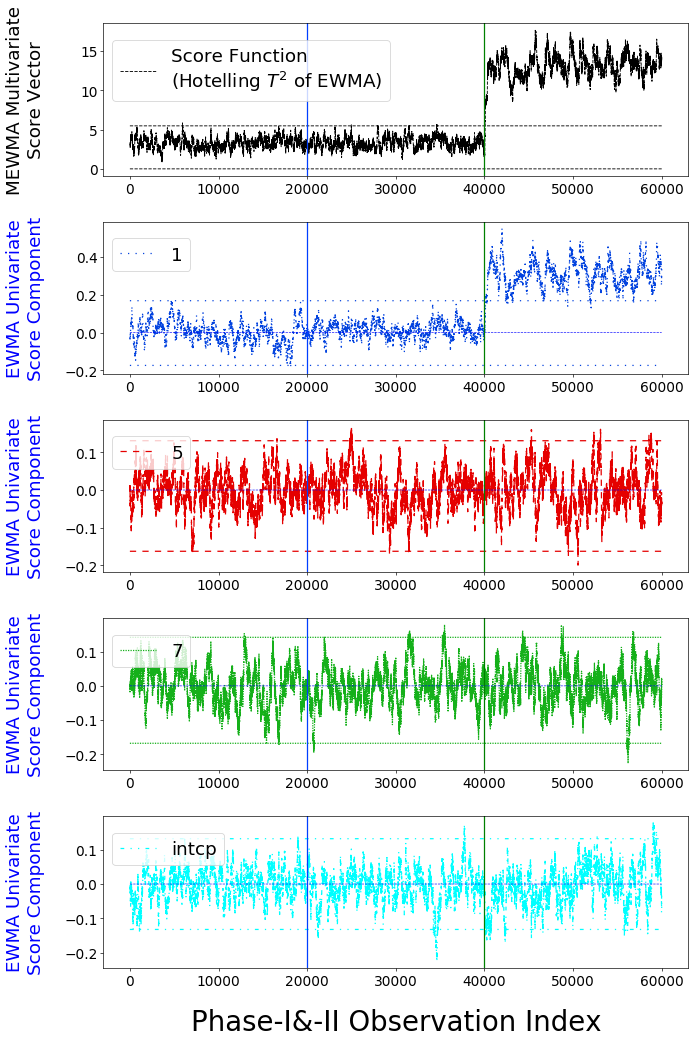
\includegraphics[width = 0.6\linewidth]{../figures/v14/sim_2/reg/neg_single_1_sim2_mlines_with_regu_1e-08_0_005.png}
%  \includegraphics[width = 0.8\linewidth]{../figures/sim_2_pinv_pdf/neg_single_sim2_mlines_with_regu_1e-08_0_005.png}
  \caption{Abrupt concept drift of linear model with independent covariates (lines are in different colors in electronic version). For conciseness, here only show MEWMA control chart of Hotelling $T^2$ (black) and EWMA control charts for the $1$st (blue), $5$th (red), $7$th (green), intercept (cyan), from the top to the bottom. The blue and green vertical lines mark the boundaries of Phase-I/II and before/after concept drift. The lines of monitored statistics in control charts have the same style and color with lines of their control limits correspondingly.}
  \label{fig:lin_reg_ind_X}
\end{figure}
In this simulation, the data set is generated by a {linear} model $y = \bm {x}^T\bm { \theta} + \epsilon$. The $10$ {covariates} {$\bm {x}=[x_1, x_2, \cdots, x _{10}]$} are independently distributed as Gaussian with mean $0$ and variance $1$; the variance of random error $ \epsilon$ is $1$; the EWMA parameter is $\lambda=0.027562$ chosen by ensuring around $50\%$ signal ratio of absolute residual after concept drift; there is no regularization in training the model because the number of parameters is small comparing to the sample size; the alarm rate for calculating the control limits is $99.9\%$; the sizes of the data set used in training, validation, Phase-I, and Phase-II are $10000$, $2000$, $20000$, and $40000$. The responses in training, validation, and Phase-I are generated with coefficients all equal to $1$. In the first half of Phase-II, the coefficients are unchanged, but in the second half, the first four coefficients are multiplied by $1- \alpha=0.7$, where $ \alpha=0.3$ is defined as the changing factor. Other coefficients are unchanged.
\begin{figure}[!htp]
\centering
%   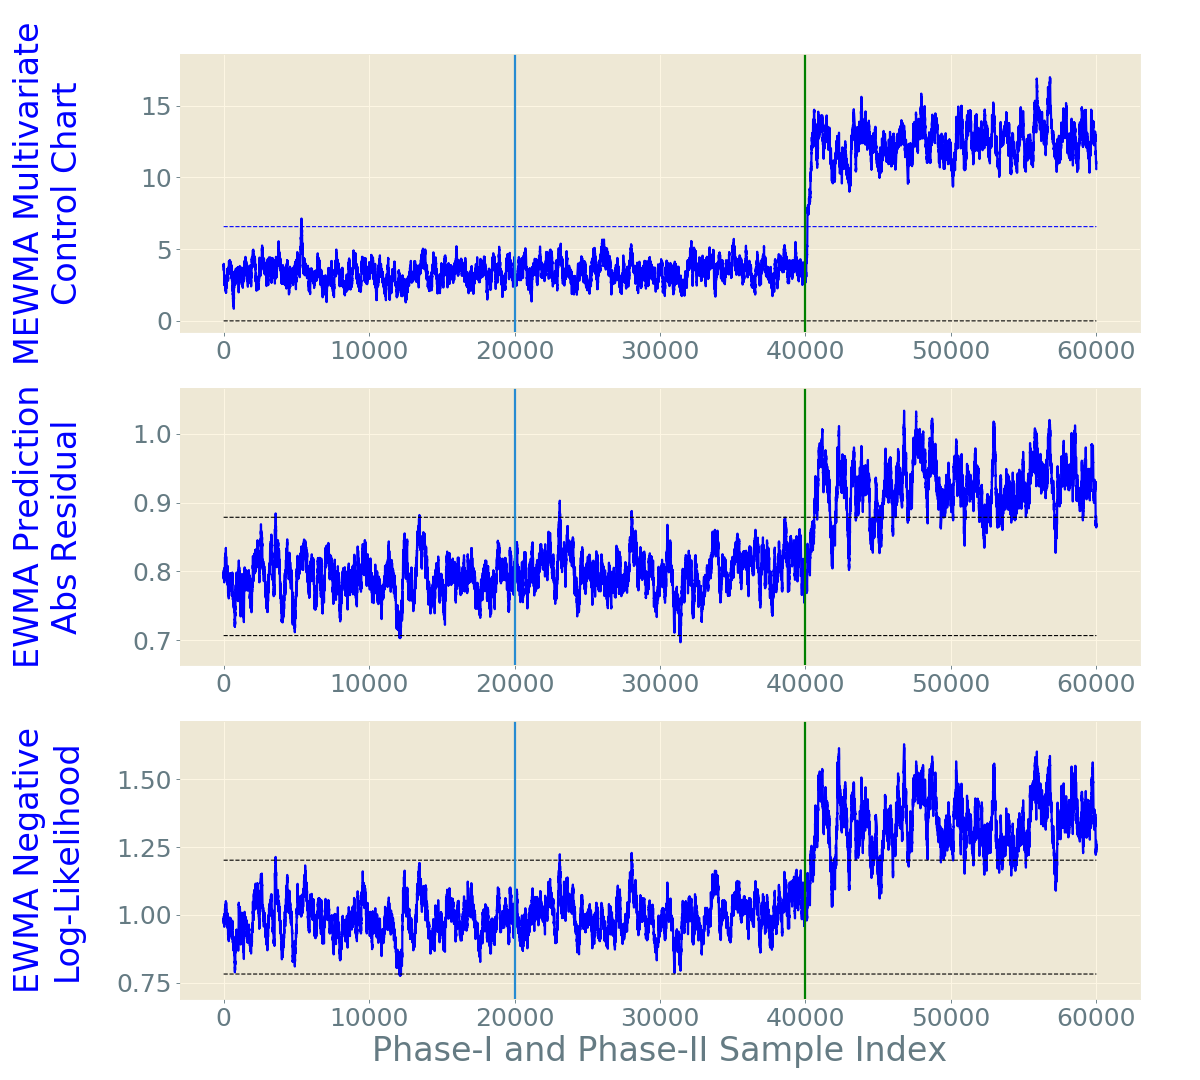
\includegraphics[width = 0.6\linewidth, trim=0in 2.6in 0in 0in, clip]{../figures/v14/sim_2/reg/3_sim2_lin_1e-08_0_005_1.png}
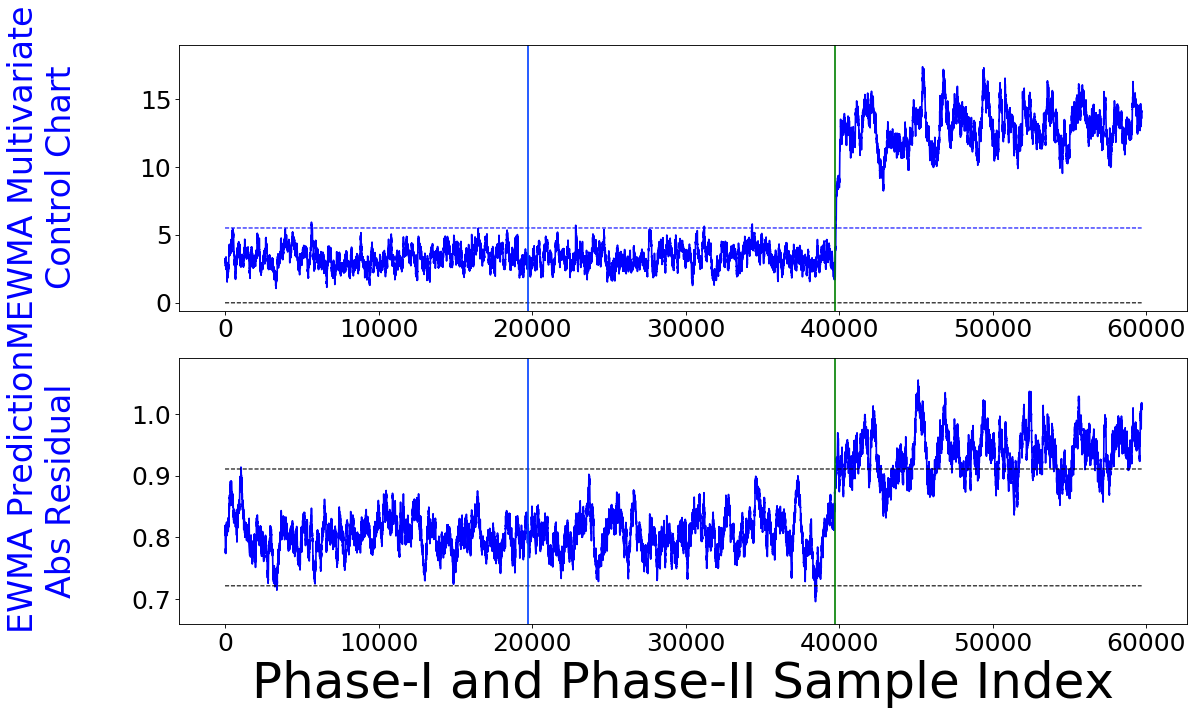
\includegraphics[width = 0.6\linewidth]{../figures/v14/sim_2/reg/1_sim2_lin_1e-08_0_005_1.png}
%  \includegraphics[width = 0.8\linewidth]{../figures/sim_2_pinv_pdf/sim2_ewma_2_metric_with_reg_1e-08_0_005.png}
%  \includegraphics[width = 0.48\linewidth]{../figures/sim_2_pinv/sim2_ewma_log_lik_with_reg_1e-08_0_005.png}
  \caption{Abrupt concept drift of linear model with independent covariates. Hotelling $T^2$ of EWMA of the score function and EWMA of the absolute residual are compared.}
  \label{fig:lin_reg_ind_X_comp}
\end{figure}

Figure~\ref{fig:lin_reg_ind_X} shows Phase-I and Phase-II of monitoring Hotelling $T^2$ and individual components of the score function. Before blue vertical lines (Phase-I), all lines of monitored statistics are well mixed in their range indicating no concept drift in training and Phase-I. After blue vertical lines (Phase-II), the EWMA lines corresponding to the first four coefficients have significant drifts (only show the first one here) and the change of mean is $0.3$ corresponding to the mean drift of coefficients, contributing to the entire line of MEWMA Hotelling $T^2$ (the black line in the top plot). In this example, all covariates are independent with others, so that there is not coupling, meaning only coefficients with concept drifts would have mean drifts. For brevity, only representative lines are shown. Lines of the rest of coefficients (including intercept) do not have mean drift but have larger deviation (or variance) after the concept drift, for the reason mentioned in Section~\ref{ss:var_infla}. The increase of deviation in control charts of those unchanged parameters results from the drifts ($\Delta \bm { \theta}$) coupling with variation of covariates ($X_k\bm {X}^T$).

To compare Hotelling $T^2$ of EWMA of the score function and EWMA of the absolute residual, we plot it with the score function respectively as shown in Figure~\ref{fig:lin_reg_ind_X_comp}. Both methods can capture the abrupt concept drift pretty well: in Phase-I they are all mixed well and in Phase-II mean drifts are close to each other. Here, we also see inflated variance of lines after the concept drift, even though they plateau very quickly. Both metrics capture the concept drift quite well, but the score-based method has higher signal ratio after concept drift, indicating that its superior performance in detecting small size changes, which is consistent with the results from Section~\ref{ss:simu_MRL}. Later, we will show results of gradual concept drift.

\item
\textbf{Abrupt Concept Drifts with Correlated Covariates}

\label{ssss:lin_not_ind_pred}
\begin{figure}[!htbp]
\centering
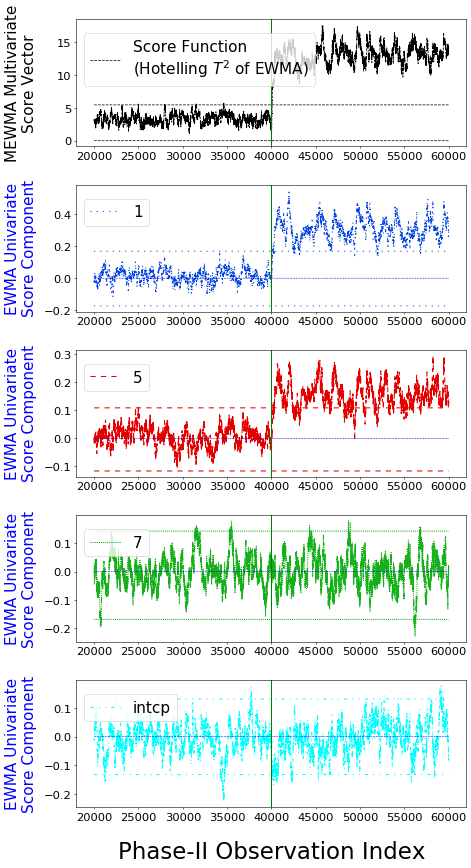
\includegraphics[width = 0.4\linewidth]{../figures/v14/sim_4/reg/PII_neg_single_1_sim4_mlines_with_regu_1e-08_0_005.png}
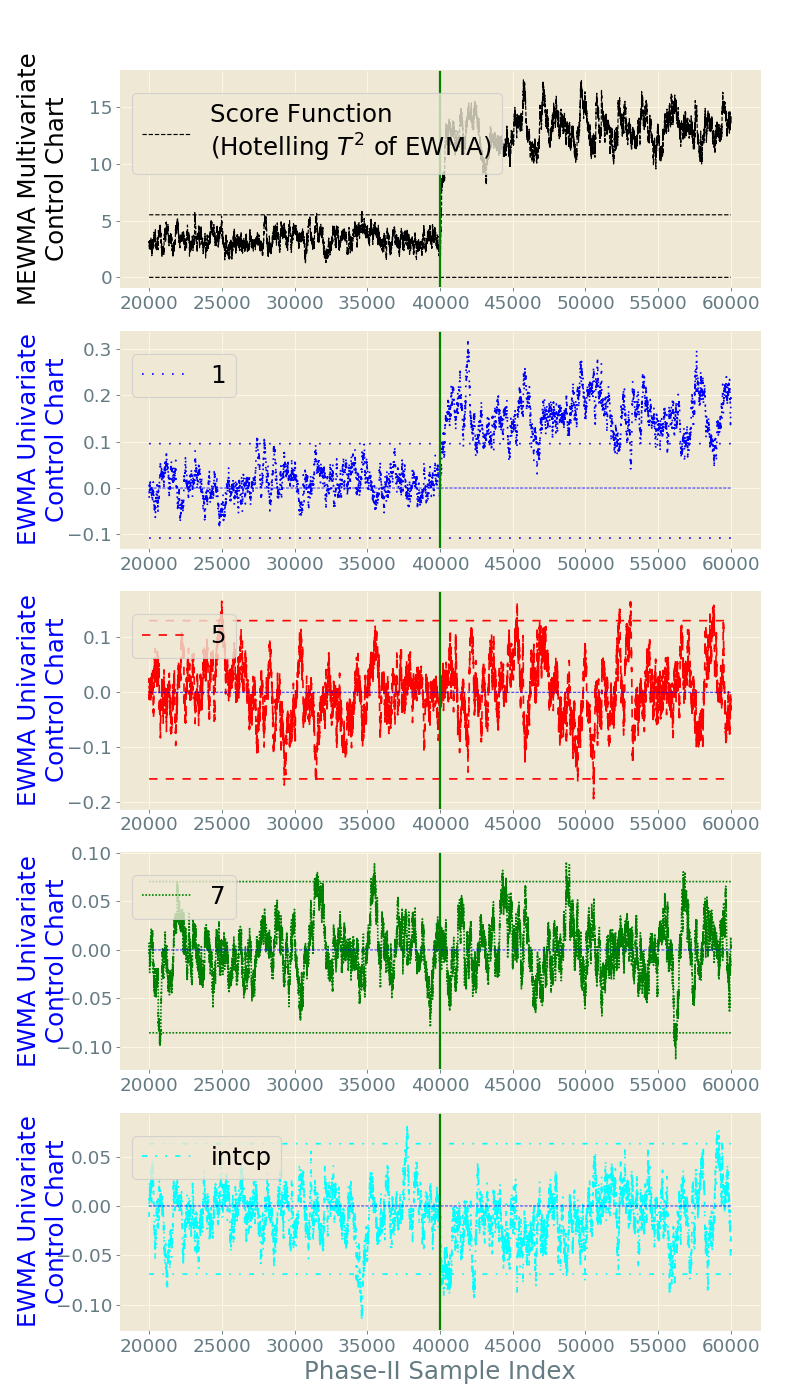
\includegraphics[width = 0.4\linewidth]{../figures/v14/sim_4/reg/PII_neg_single_1_sim4_fisher_mlines_with_regu_1e-08_0_005.png}
%\includegraphics[width = 0.4\linewidth]{../figures/sim_4_1_pinv_pdf/PII_neg_single_sim4_mlines_with_regu_1e-08_0_005.png}
%\includegraphics[width = 0.4\linewidth]{../figures/sim_4_1_pinv_pdf/PII_pos_single_sim4_mlines_fisher_with_regu_1e-08_0_005.png}
%  \includegraphics[width = 1\linewidth]{../figures/sim_3/PII_pos_sim3_mlines_with_regu_1e-08_0_001.png}
%  \includegraphics[width = 1\linewidth]{../figures/sim_3/PII_neg_sim3_mlines_fisher_with_regu_1e-08_0_001.png}
  \caption{Abrupt concept drift of linear model with correlated {covariates} (lines are in different colors in electronic version). Comparison are made between before (left) and after (right) being transformed by {the inverse of the estimated} Fisher Information Matrix, {$\mathbf {I} ( {\bm{\theta}} ^{(0)})$.} For legibility, here only show MEWMA control chart of Hotelling $T^2$ (black) and EWMA control charts for the $1$st (blue), $5$th (red), $7$th (green), intercept (cyan), from the top to the bottom. The lines of monitored statistics in control charts have the same style and color with lines of their control limits correspondingly.}
  \label{fig:lin_reg_not_ind_X}
\end{figure}
Then, we manually introduce correlation between {covariates} by setting $0.5 x_1 + 0.5 x_5$ and $ 0.3 x_1 + 0.3 x_2 + 0.4 x_6$ as new $x_5$ and $x_6$ respectively, with others remaining the same. The EWMA and MEWMA control charts before (left) and after (right) transformed by {the inverse of the estimated} ${\mathbf {I}}(\bm { \theta}^{(0)})$ is as shown in Figure~\ref{fig:lin_reg_not_ind_X}. The blue (the $2$nd plot) and green lines (the $4$th plot) are for $x_1$ and $x_5$: transforming or not has no effect on those lines, where the coefficient for $x_1$ has mean {drift} but $x_7$ does not. However, according to the red line (the $3$rd plot) for $x_5$, transformation changes it from having mean {drift} to not, indicating that this transformation successfully decouples concept drift from correlated covariates. This is not surprising, because ${\mathbf {I}} ^{-1}(\bm { \theta}^{(0)})$ equals to $E ^{-1} [\bm {X}\bm {X}^T]$, which does not depend on $ \bm { \theta} ^{(0)}$ or $ \bm { \theta} ^{(1)}$, meaning high-ordered term in the equation~(\ref{eqn:cd_decomp_fisher_approx}) is zero. However, in the next experiment for logistic regression, the concept drift is harder to decouple because multiplying ${\mathbf {I}} ^{-1}(\bm { \theta}^{(0)})$ can only approximately decouple concept drifts.

\item
\textbf{Gradual Concept Drifts with Correlated Covariates}
\label{ssss:lin_not_ind_pred_grad_cd}
\begin{figure}[!htbp]
\centering
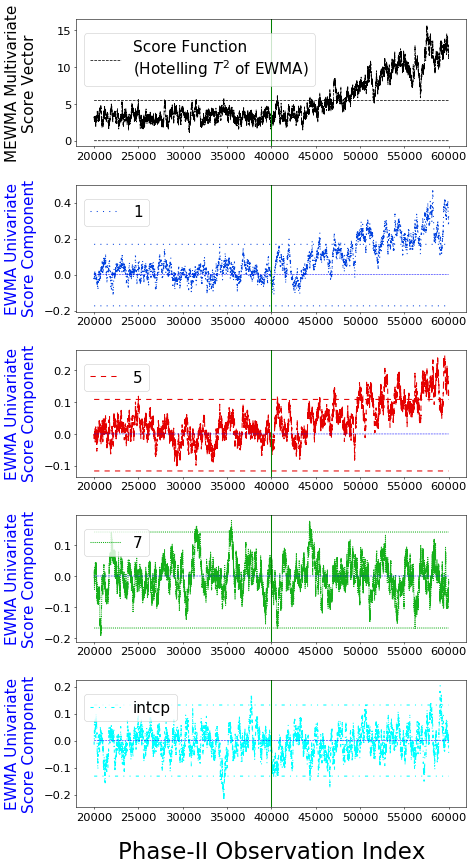
\includegraphics[width = 0.4\linewidth]{../figures/v14/sim_6/reg/PII_neg_single_1_sim6_mlines_with_regu_1e-08_0_005.png}
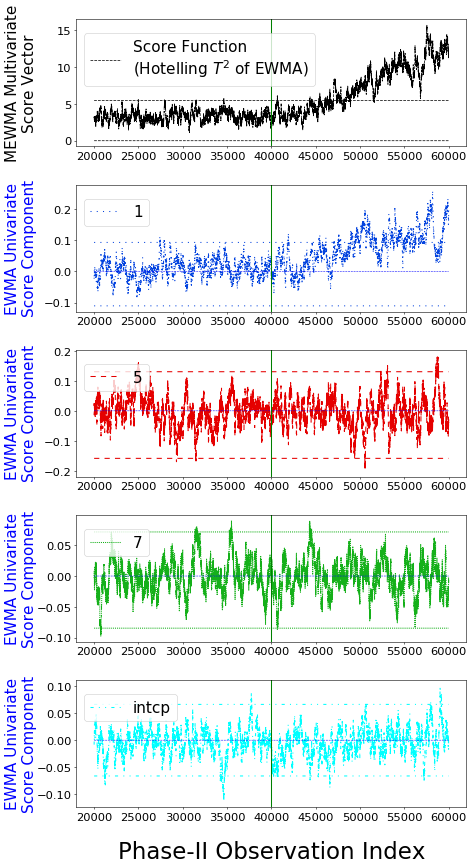
\includegraphics[width = 0.4\linewidth]{../figures/v14/sim_6/reg/PII_neg_single_1_sim6_fisher_mlines_with_regu_1e-08_0_005.png}
%\includegraphics[width = 0.4\linewidth]{../figures/sim_6_1_pinv_pdf/PII_neg_single_sim6_mlines_with_regu_1e-08_0_005.png}
%\includegraphics[width = 0.4\linewidth]{../figures/sim_6_1_pinv_pdf/PII_pos_single_sim6_mlines_fisher_with_regu_1e-08_0_005.png}
 \caption{Gradual concept drift of linear model with correlated {covariates} (lines are in different colors in electronic version). Comparison are made between before (left) and after (right) being transformed by {the inverse of the estimated} Fisher Information Matrix, {$\mathbf {I} ( {\bm{\theta}} ^{(0)})$.} For legibility, here only show MEWMA control chart of Hotelling $T^2$ (black) and EWMA control charts for the $1$st (blue), $5$th (red), $7$th (green), intercept (cyan), from the top to the bottom. The left (right) vertical axis is for univariate (multivariate) control charts. The lines of monitored statistics in control charts have the same style and color with lines of their control limits correspondingly.}
  \label{fig:lin_reg_not_ind_X_grad_cd}
\end{figure}

In real applications, many concept drifts happen in a gradual way. In this data set, all conditions are the same with that in the Section~\ref{ssss:lin_not_ind_pred} except that the concept drifts happen linearly in the second half time of Phase-II. The starting and ending coefficients of the linear concept drift period correspond to those before and after concept drifts in the abrupt case. 
\begin{figure}[!htbp]
\centering
% \includegraphics[width = 0.48\linewidth]{../figures/sim_6_1_pinv_pdf/sim6_ewma_resi_with_reg_1e-08_0_005.png}
%\includegraphics[width = 0.8\linewidth]{../figures/sim_6_1_pinv_pdf/sim6_ewma_2_metric_with_reg_1e-08_0_005.png}
% 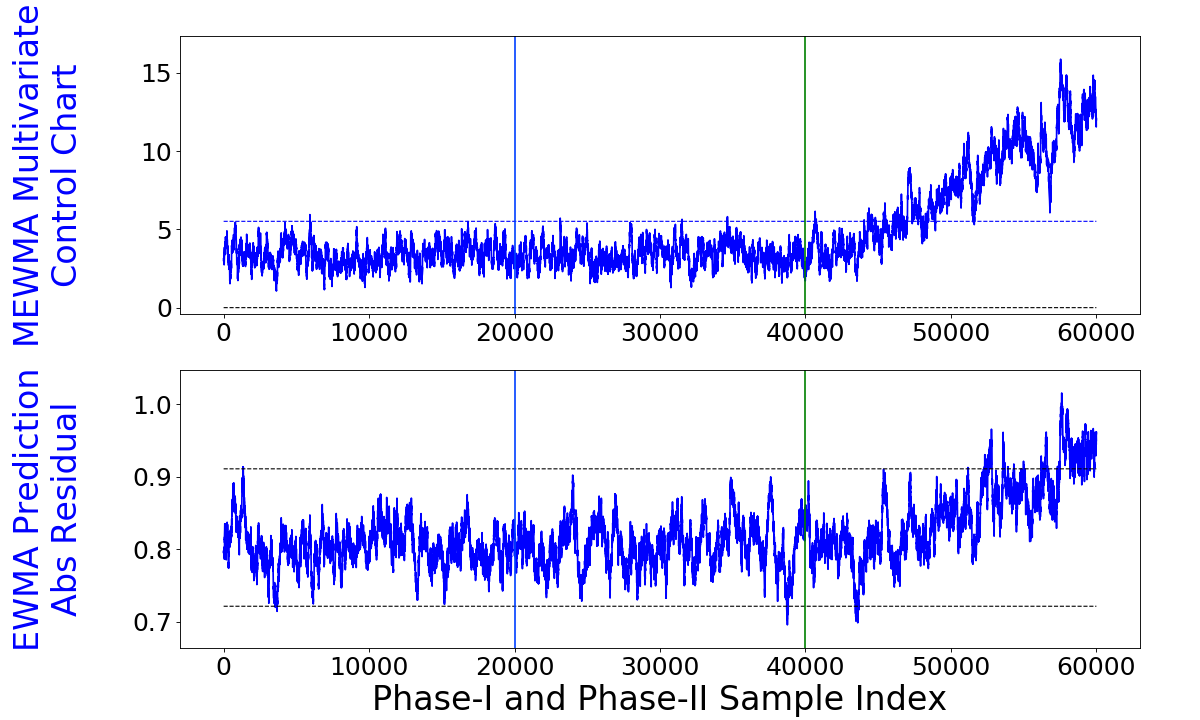
\includegraphics[width = 0.6\linewidth, trim=0in 2.6in 0in 0in, clip]{../figures/v14/sim_6/reg/1_sim6_lin_1e-08_0_005_1.png}
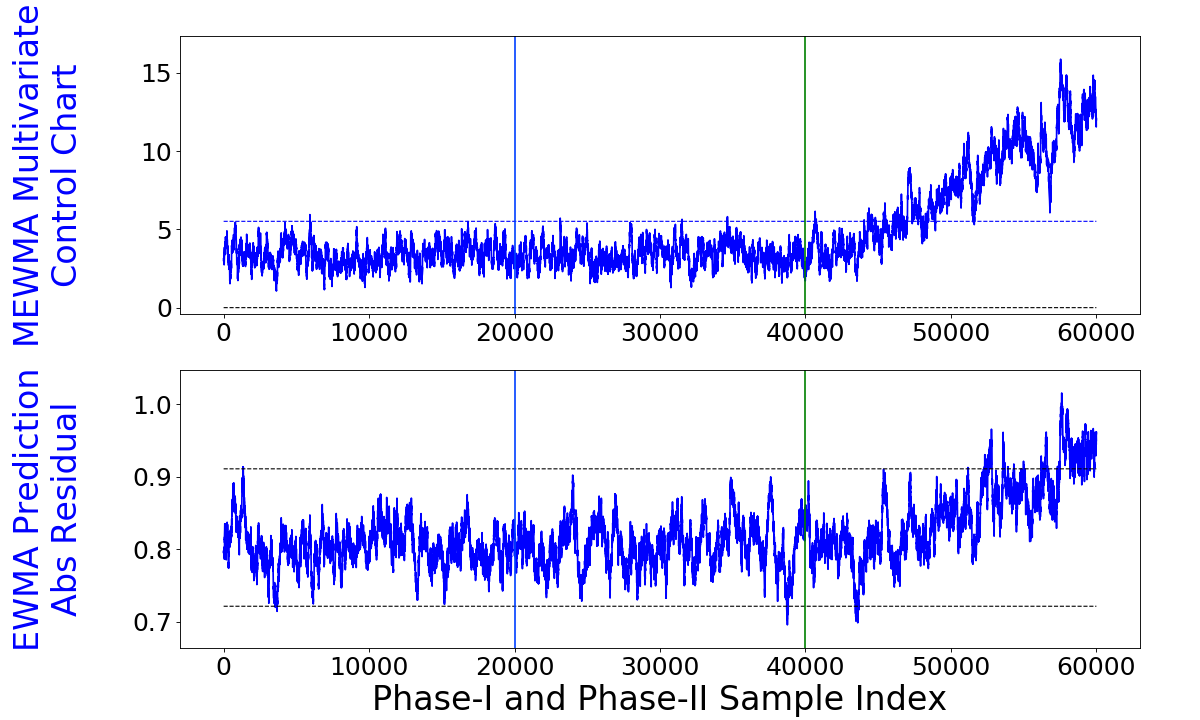
\includegraphics[width = 0.6\linewidth]{../figures/v14/sim_6/reg/1_sim6_lin_1e-08_0_005_1.png}
  \caption{Gradual concept drift of linear model with correlated covariates. Hotelling $T^2$ of EWMA of the score function and EWMA of the absolute residual are compared.}
  \label{fig:lin_reg_ind_X_grad_cd_comp}
\end{figure}

The EWMA and MEWMA control charts before (left) and after (right) transformed by {the inverse of the estimated} ${\mathbf {I}}(\bm { \theta}^{(0)})$ is as shown in Figure~\ref{fig:lin_reg_not_ind_X_grad_cd}. Similarly with that in the Section~\ref{ssss:lin_not_ind_pred}, lines corresponding to covariates with true concept drifts or independent with others are not affected by transformation in terms whether concept drifts show up in control charts. In Figure~\ref{fig:lin_reg_ind_X_grad_cd_comp}, we see that monitoring the score vectors gives an earlier detection of the starting position of the concept drift than EWMA of the absolute residual.
\end{enumerate}

\subsubsection{Simulated data set for Logistic Regression}
\label{sss:logi_exp}
\begin{enumerate}[(I)]
\item
\textbf{Abrupt Concept Drifts with Independent Covariates}
\label{ssss:log_ind_pred}
\begin{figure}[!htbp]
\centering
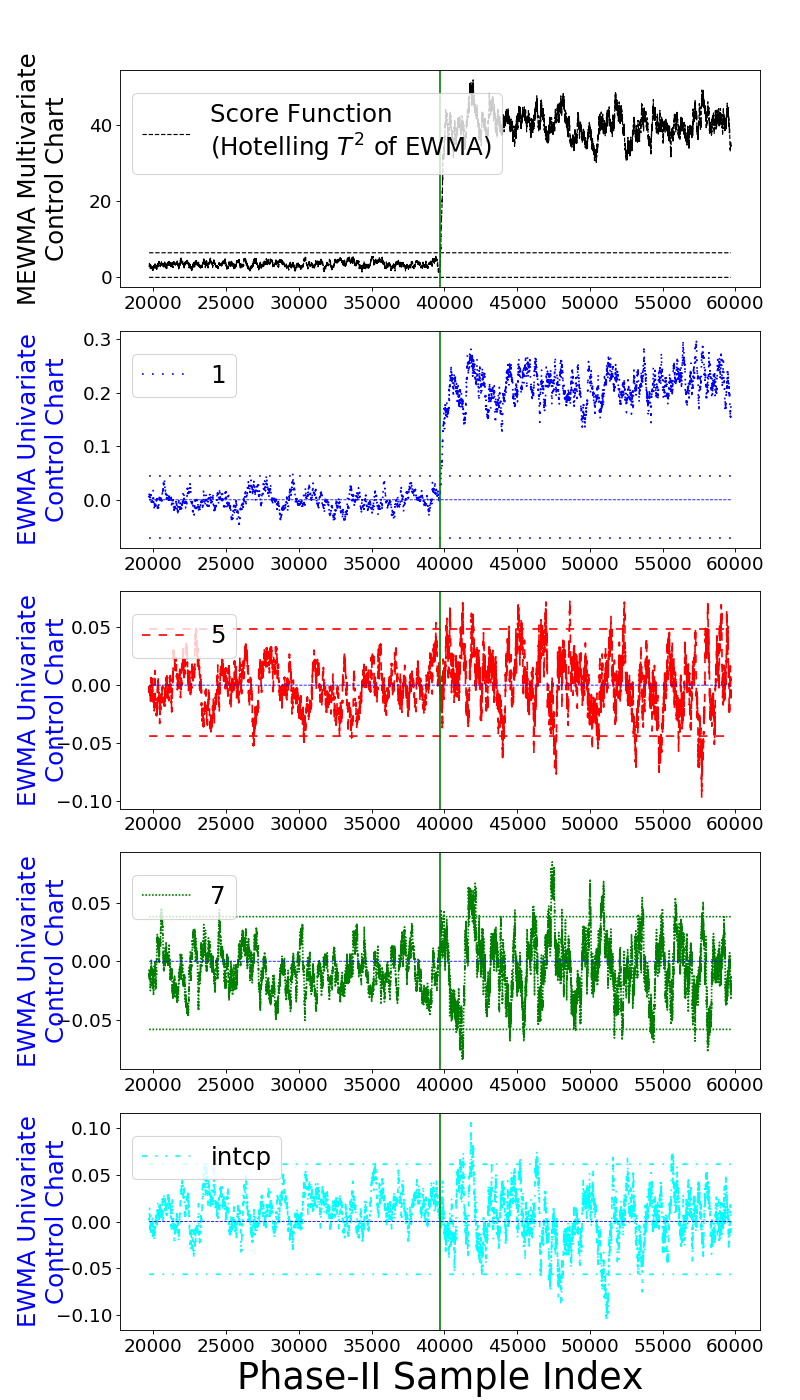
\includegraphics[width = 0.4\linewidth]{../figures/v14/sim_5/logi_no_muco/PII_pos_single_1_sim5_mlines_with_regu_1e-08_0_005.png}
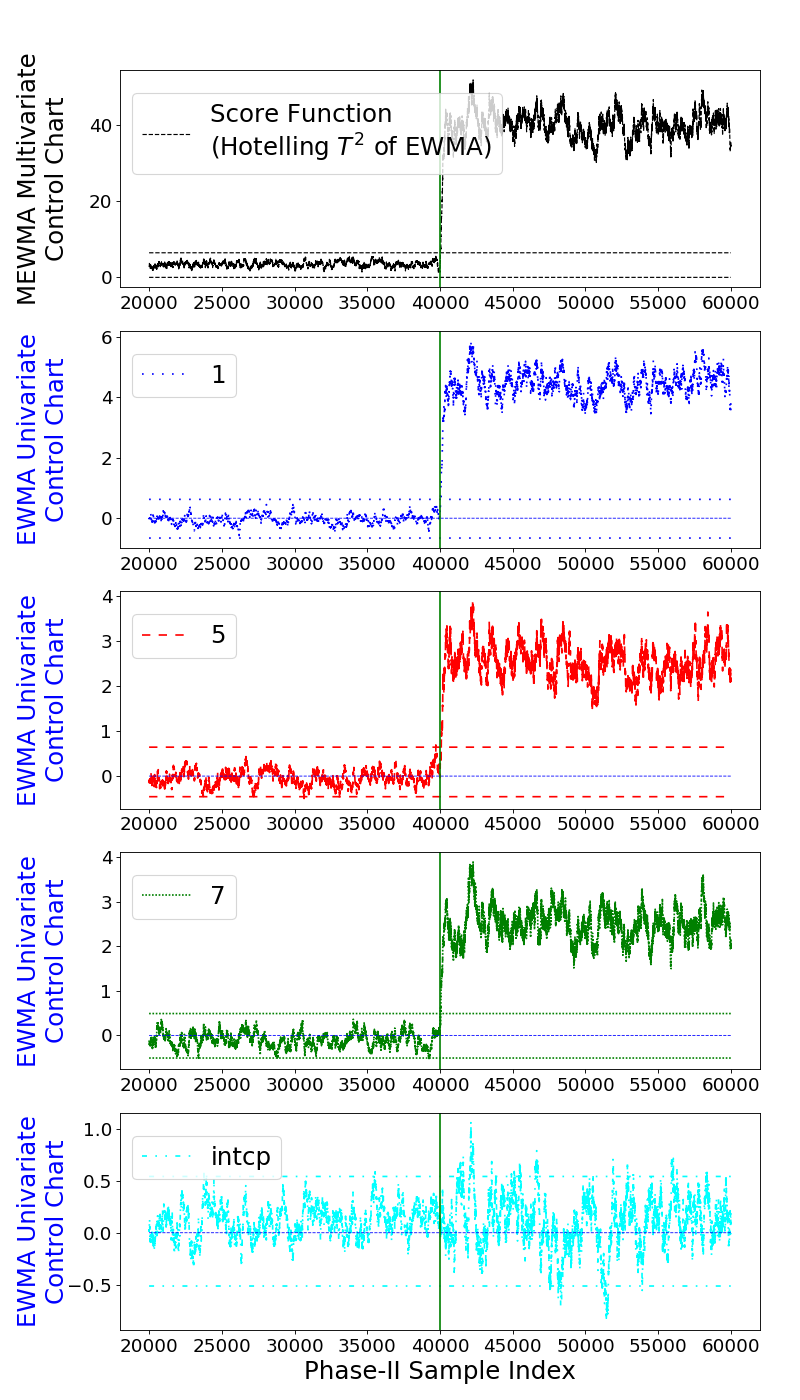
\includegraphics[width = 0.4\linewidth]{../figures/v14/sim_5/logi_no_muco/PII_pos_single_1_sim5_fisher_mlines_with_regu_1e-08_0_005.png}
%\includegraphics[width = 0.4\linewidth]{../figures/sim_3_pinv_pdf/PII_pos_single_sim3_mlines_with_regu_1e-08_0_005.png}
%\includegraphics[width = 0.4\linewidth]{../figures/sim_3_pinv_pdf/PII_neg_single_sim3_mlines_fisher_with_regu_1e-08_0_005.png}
%  \includegraphics[width = 1\linewidth]{../figures/sim_3/PII_pos_sim3_mlines_with_regu_1e-08_0_001.png}
%  \includegraphics[width = 1\linewidth]{../figures/sim_3/PII_neg_sim3_mlines_fisher_with_regu_1e-08_0_001.png}
  \caption{Abrupt concept drift of logistic regression with independent {covariates} (lines are in different colors in electronic version). Comparison are made between before (left) and after (right) being transformed by {the inverse of the estimated} Fisher Information Matrix, {$\mathbf {I} ( {\bm{\theta}} ^{(0)})$.} For legibility, here only show MEWMA control chart of Hotelling $T^2$ (black) and EWMA control charts for the $1$st (blue), $5$th (red), $7$th (green), intercept (cyan), from the top to the bottom. The lines of monitored statistics in control charts have the same style and color with lines of their control limits correspondingly.}
  \label{fig:log_reg_ind_X}
\end{figure}

This simulated data set has the same parameter as that in the corresponding Experiment~\ref{ssss:lin_ind_pred} in Section~\ref{sss:lin_exp}, except that here the model becomes {logistic model} {$p(y=1|\bm {x})= \sigma (\bm {x}^T\bm { \theta})$,} where $\sigma (\cdot)$ is the sigmoid function.
\begin{figure}[!htbp]
\centering
% 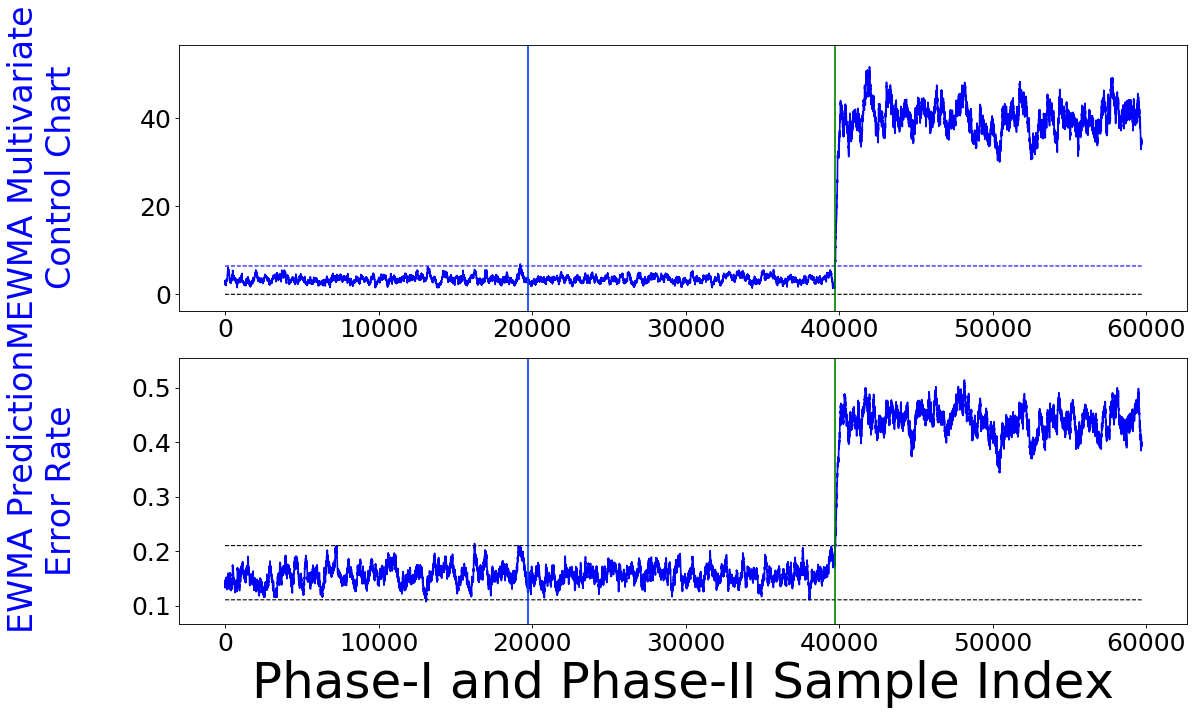
\includegraphics[width = 0.6\linewidth, trim=0in 2.6in 0in 0in, clip]{../figures/v14/sim_5/logi_no_muco/1_sim5_logi_1e-08_0_005_1.png}
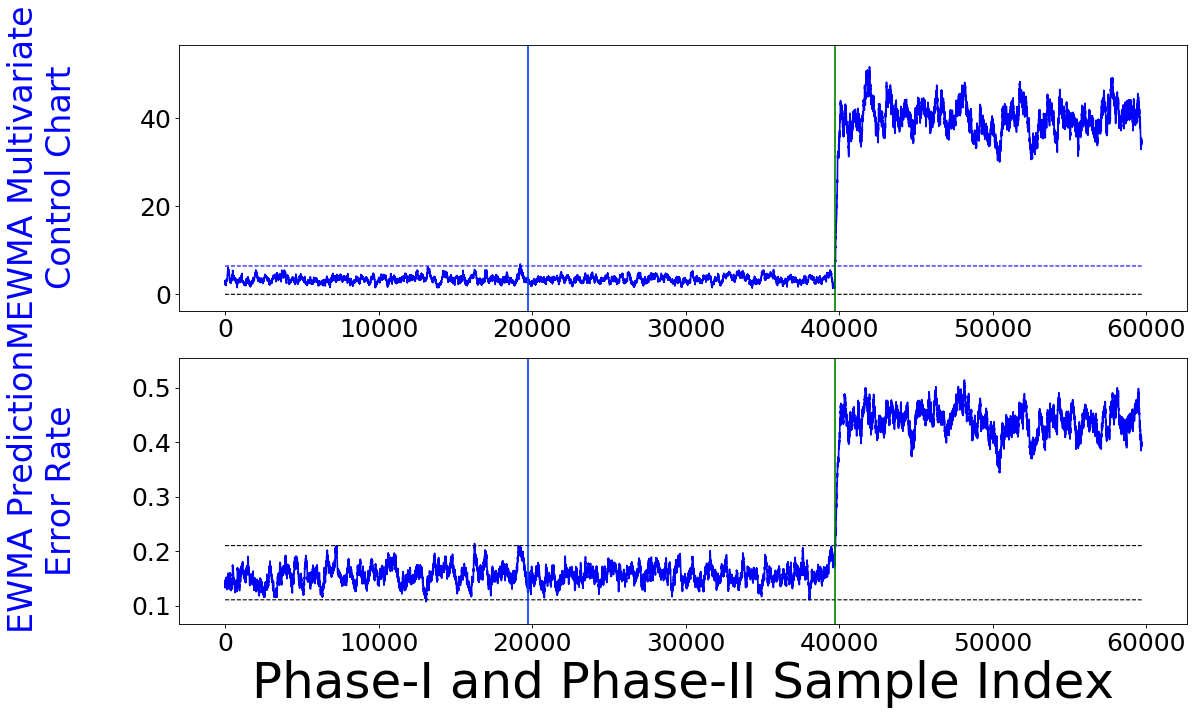
\includegraphics[width = 0.6\linewidth]{../figures/v14/sim_5/logi_no_muco/1_sim5_logi_1e-08_0_005_1.png}
%  \includegraphics[width = 0.49\linewidth]{../figures/sim_3_pinv_pdf/sim3_ewma_2_metric_with_reg_1e-08_0_005.png}
%  \includegraphics[width = 0.49\linewidth]{../figures/sim_3_pinv_pdf/sim3_ewma_2_metric_with_reg_1e-08_0_002.png}
%  \includegraphics[width = 0.24\linewidth]{../figures/sim_3_pinv_pdf/sim3_ewma_dev_with_reg_1e-08_0_005.png}
%  \includegraphics[width = 0.24\linewidth]{../figures/sim_3_pinv_pdf/sim3_ewma_dev_with_reg_1e-08_0_001.png}
  \caption{Abrupt concept drift of logistic regression with independent covariates. Hotelling $T^2$ of EWMA of the score function and EWMA of the error rate are compared.}
  \label{fig:log_reg_ind_X_comp}
\end{figure}

As shown in Figure~\ref{fig:log_reg_ind_X}, even though components of $\bm {x}$ are independent, the concept drifts of the first four components still propagate to the rest (with smaller magnitude) which do not have drifts, except the intercept (because of the symmetry of distribution of our simulated $\bm {x}$). This is because $E [ (\sigma ( \bm {X}^T\bm { \theta}^{(1)} ) - \sigma ( \bm {X}^T\bm { \theta}^{(0)} )) \bm {X}] $ is nonlinear and depends on parameters. This is supported by the comparison of the left and right column in Figure~\ref{fig:log_reg_ind_X}: applying transformation matrix cannot recover zero mean drift for those covariates without concept drift (the red line in the $3$rd plot for $x_5$) meaning this coupling is due to the nonlinearity rather than correlation between covariates in Experiment~\ref{ssss:lin_not_ind_pred} in Section~\ref{sss:lin_exp}. During experiments, we find an interesting special case that if the concept drift is restricted to flipping sign of coefficients, the covariates without concept drift will not have mean {drift} (no coupling effect) in those control charts, due to the same reason that the intercept has no mean drift, mentioned above.

As the comparison in Experiment~\ref{ssss:lin_ind_pred} in Section~\ref{sss:lin_exp}, in Figure~\ref{fig:log_reg_ind_X_comp}, Hotelling $T^2$ of EWMA of the score function and EWMA of the prediction error, both methods can capture the abrupt concept drift, but the EWMA of the prediction error has much less signal ratio. This is because in Phase-I the prediction error has a wider range between control limits than that of the score function, so that in Phase-II the control chart is less sensitive to the deviation.

\item
\textbf{Abrupt Concept Drifts with Correlated Covariates}
\label{ssss:log_not_ind_pred}

\begin{figure}[!htbp]
\centering
\includegraphics[width = 0.4\linewidth]{../figures/v14/sim_5/logi/PII_pos_single_1_sim5_mlines_with_regu_1e-08_0_005.png}
\includegraphics[width = 0.4\linewidth]{../figures/v14/sim_5/logi/PII_pos_single_1_sim5_fisher_mlines_with_regu_1e-08_0_005.png}
%  \includegraphics[width = 0.4\linewidth]{../figures/sim_3_1_pinv_pdf/PII_pos_single_sim3_mlines_with_regu_1e-08_0_005.png}
%  \includegraphics[width = 0.4\linewidth]{../figures/sim_3_1_pinv_pdf/PII_neg_single_sim3_mlines_fisher_with_regu_1e-08_0_005.png}
  \caption{Abrupt concept drift of logistic regression with correlated {covariates} (lines are in different colors in electronic version). Comparison are made between before (left) and after (right) being transformed by {the inverse of the estimated} Fisher Information Matrix, {$\mathbf {I} ( {\bm{\theta}} ^{(0)})$.} For legibility, here only show MEWMA control chart of Hotelling $T^2$ (black) and EWMA control charts for the $1$st (blue), $5$th (red), $7$th (green), intercept (cyan), from the top to the bottom. The lines of monitored statistics in control charts have the same style and color with lines of their control limits correspondingly.
% Concept drift of logistic regression with correlated {covariates} (lines are in different colors in electronic version). Comparison are made between before (above) and after (below) being transformed by {the inverse of the estimated} Fisher Information Matrix, {$\mathbf {I} ( {\bm{\theta}} ^{(0)})$.} 
}
  \label{fig:log_reg_not_ind_X}
\end{figure}

As in Experiment~\ref{ssss:lin_not_ind_pred} above, we introduce correlation between {covariates.} The comparison between before and after transformation with {the inverse of the estimated} {$\mathbf {I} ( {\bm{\theta}} ^{ (0)}) = E [{p} (\bm {X},\bm { \theta} ^{ (0)}) (1-{p}(\bm {X},\bm { \theta} ^{ (0)})) \bm {X} \bm {X}^T] \Delta \bm{ \theta}$}, where {$p (\bm {X},\bm { \theta} ^{ (0)}) = \sigma ( \bm {X}^T\bm { \theta} ^{ (0)})$}, is shown in Figure~\ref{fig:log_reg_not_ind_X}. The transformation makes the mean {drift} uniformly significant on control charts over all {covariates,} no matter whether they have concept drift (here only show representative lines). For the $x_7$ component (green in the $4$th plot), previously mild concept drift due to nonlinearity becomes even larger (worse) after transformation. This indicates that the approximation in the equation (\ref{eqn:cd_decomp_fisher_approx}) is not accurate. This makes sense, because the concept drift is large (coefficients from $1$ to $-1$), violating the assumption of ``small higher-ordered terms of concept drift". 

\item
\textbf{Concept Drifts with Correlated Covariates and an Assumption}
\label{ssss:log_not_ind_pred_assum}
\begin{figure}[!htbp]
\centering
\includegraphics[width = 0.4\linewidth]{../figures/v14/sim_5/logi_small/PII_pos_single_1_sim5_mlines_with_regu_1e-08_0_005.png}
\includegraphics[width = 0.4\linewidth]{../figures/v14/sim_5/logi_small/PII_pos_single_1_sim5_fisher_mlines_with_regu_1e-08_0_005.png}
%  \includegraphics[width = 0.4\linewidth]{../figures/sim_5_1_pinv_pdf/PII_pos_single_sim5_mlines_with_regu_1e-08_0_005.png}
%  \includegraphics[width = 0.4\linewidth]{../figures/sim_5_1_pinv_pdf/PII_neg_single_sim5_mlines_fisher_with_regu_1e-08_0_005.png}
  \caption{
 Abrupt concept drift of logistic regression with correlated covariates (lines are in different colors in electronic version). Simulated data are modified to reduce the magnitude of $ \bm {x}_i^T\bm { \theta}^{(1)}$ and $  \bm {x}_i^T\bm { \theta}^{(0)}$. Comparison are made between before (left) and after (right) being transformed by the inverse of the estimated Fisher Information Matrix, $\mathbf {I} ( {\bm{\theta}} ^{(0)})$. For legibility, here only show MEWMA control chart of Hotelling $T^2$ (black) and EWMA control charts for the $1$st (blue), $5$th (red), $7$th (green), intercept (cyan), from the top to the bottom. The lines of monitored statistics in control charts have the same style and color with lines of their control limits correspondingly.
%Concept drift of logistic regression with correlated covariates.  Simulated data are modified to reduce the magnitude of $ \bm {x}_i^T\bm { \theta}^{ (1)}$ and $  \bm {x}_i^T\bm { \theta}^{ (0)}$. Comparison are made between before (above) and after (below) being transformed by the inverse of the estimated Fisher Information Matrix, $\mathbf {I} ( {\bm{\theta}} ^{(0)})$. 
}
  \label{fig:log_reg_not_ind_X_1}
\end{figure}

To resolve the failure of diagnosing true concept drifts in Experiment~\ref{ssss:log_not_ind_pred}, we observe that, according to the mean drift of logistic regression $E [ (\sigma (\bm {X}^T\bm { \theta}^{ (1)}) - \sigma ( \bm {X}^T\bm { \theta}^{ (0)})) \bm {X}] $, if $ \bm {x}^T\bm { \theta}^{ (1)}$ and $ \bm {x}^T\bm { \theta}^{ (0)}$ are all relative small (say $\ll 4$ in absolute value), the sigmoid function $ \sigma (\cdot)$ are in the linear region, so that we can approximate the mean drift by $E [ (\sigma ( \bm {X}^T\bm { \theta}^{ (1)} ) - \sigma ( \bm {X}^T\bm { \theta}^{ (0)} )) \bm {X}] \approx E [ \eta( \bm {X}^T\bm { \theta}^{ (1)} -  \bm {X}^T\bm { \theta}^{ (0)} ) \bm {X}] = \eta E[\bm{XX}^T] \Delta \bm { \theta} $, where $ \eta$ is just a scalar constant factor, reducing to the case of linear model, as in Section~\ref{sss:lin_exp}.  

To test this argument, we follow the data set generating process in Experiment~\ref{ssss:log_not_ind_pred} in Section~\ref{sss:lin_exp} but make modifications as below: the coefficients of all covariates in training, validation, Phase-I, and the first half period of Phase-II changes to $0.2$; in the second half period of Phase-II, the coefficients of the first four covariates are multiplied by $-1$. In Figure~\ref{fig:log_reg_not_ind_X_1}, we observe that, transforming or not does not change the lines corresponding to covariates which are independent with others or truly have concept drifts in terms of whether to show concept drifts in control charts (the coefficient for $x_1$ (blue in the $2$nd plot) has mean drift but $x_7$ (green in the $4$th plot) and intercept (cyan in the last plot) does not); but transformation changes the line $x_5$ (red in the $3$rd plot) in the control charts from having mean drift to not. In other words, the concept drifts are successfully decoupled. Due to the reduced variance of covariates and smaller concept drifts, the variance inflation after concept drifts is also mitigated, as shown in the second half of Phase-II. Even though this requires some assumption, this property of logistic regression is still practically valuable, because when arguments of sigmoid function have large absolute value, large concept drifts may not have much impact on the performance of predictive models (the sigmoid function is in the plateau regions), while when the sigmoid function is in linear region, small drifts in coefficients can significantly change prediction, so that we might want to understand which covariates contribute to such change.

This property of logistic regression can be extended to gradual concept drifts. Modifying the above data set as done in Experiment~\ref{ssss:lin_not_ind_pred_grad_cd} in Section~\ref{sss:lin_exp}, meaning change the abrupt concept drift to linear one.
\begin{figure}[!htbp]
\centering
\includegraphics[width = 0.4\linewidth]{../figures/v14/sim_7/logi_small/PII_pos_single_1_sim7_mlines_with_regu_1e-08_0_005.png}
\includegraphics[width = 0.4\linewidth]{../figures/v14/sim_7/logi_small/PII_pos_single_1_sim7_fisher_mlines_with_regu_1e-08_0_005.png}
%\includegraphics[width = 0.4\linewidth]{../figures/sim_7_1_pinv_pdf/PII_pos_single_sim7_mlines_with_regu_1e-08_0_005.png}
%\includegraphics[width = 0.4\linewidth]{../figures/sim_7_1_pinv_pdf/PII_neg_single_sim7_mlines_fisher_with_regu_1e-08_0_005.png}
 \caption{Gradual concept drift of logistic regression with correlated {covariates} (lines are in different colors in electronic version). Comparison are made between before (left) and after (right) being transformed by {the inverse of the estimated} Fisher Information Matrix, {$\mathbf {I} ( {\bm{\theta}} ^{(0)})$.} For legibility, here only show MEWMA control chart of Hotelling $T^2$ (black) and EWMA control charts for the $1$st (blue), $5$th (red), $7$th (green), intercept (cyan), from the top to the bottom. The lines of monitored statistics in control charts have the same style and color with lines of their control limits correspondingly.}
  \label{fig:log_reg_not_ind_X_grad_cd}
\end{figure}
\begin{figure}[!htbp]
\centering
% \includegraphics[width = 0.6\linewidth, trim=0in 2.6in 0in 0in, clip]{../figures/v14/sim_7/logi_small/1_sim7_logi_1e-08_0_005_1.png}
\includegraphics[width = 0.6\linewidth]{../figures/v14/sim_7/logi_small/1_sim7_logi_1e-08_0_005_1.png}
% \includegraphics[width = 0.8\linewidth]{../figures/sim_7_1_pinv_pdf/sim7_ewma_2_metric_with_reg_1e-08_0_005.png}
%\includegraphics[width = 0.48\linewidth]{../figures/sim_7_1_pinv_pdf/sim7_ewma_dev_with_reg_1e-08_0_005.png}
  \caption{Gradual concept drift of logistic regression with correlated covariates. Hotelling $T^2$ of EWMA of the score function and EWMA of the absolute residual are compared.}
  \label{fig:log_reg_ind_X_grad_cd_comp}
\end{figure}

The MEWMA and EWMA control charts before (left) and after (right) transformed by {the inverse of the estimated} ${\mathbf {I}}(\bm { \theta}^{(0)})$ is as shown in Figure~\ref{fig:log_reg_not_ind_X_grad_cd}. Similarly with that in Figure \ref{fig:log_reg_not_ind_X_1}, lines corresponding to covariates with true concept drifts or independent with others are not affected by transformation in terms whether to show concept drifts in figures, confirming the validity of the assumption in this section. In Figure~\ref{fig:log_reg_ind_X_grad_cd_comp}, we see that monitoring the score vectors renders an even much earlier detection of the starting position of the concept drift than EWMA of the prediction error rate.

In summary, we demonstrated the efficacy of using MEWMA control charts to monitor the score function in detecting concept drifts. And we also show how to diagnose the concept drifts by applying proper transformation and EWMA control charts. Also, we discussed the coupling due to multicollinearity and nonlinearity and how to resolve those issues. The practicability of the assumption of small argument for decoupling concept drifts in logistical regression was also justified. Next, this method will be considered and used in two real data sets.
\end{enumerate}

\section{Real Data Examples}
\label{s:real_data}
Concept drifts are usually hard to directly testify in real life, because the existence of concept drift results from some hidden effects or contexts that are not available beforehand. However, for the purpose of testing our methods, we choose two examples that has generally accepted posterior that can be used as evidence of concept drifts. One is a data set of credit default from a major financial company from $2003$ to $2008$ during which the subprime mortgage crisis happened. And the other is a data set of Capital Bikeshare from $2010$ to $2020$ during which ``sharing economy" is expanding rapidly. Those two data sets correspond to ``abrupt" and ``gradual" concept drift, which will be elaborated in details after we giving examples.

In this section, we will apply the monitoring and diagnosis procedures mentioned above to two real data sets, and provide a real case study in how these methods can improve our understanding or model performance.

\subsection{Credit Risk data set}
\label{ss:cr_ds}
\begin{figure}[!htbp]
\centering
%  \includegraphics[width = 0.49\linewidth]{../figures/v14/credit_default/lin_model_pinv_pdf/credit_ewma_2_metric_with_reg_21_544346128_0_001.png}
% 	\includegraphics[width = 0.49\linewidth, trim=0in 2.6in 0in 0in, clip]{../figures/v14/credit_default/logi_scal_train_PI/credit_logi_1e-08_0_0001_0_001_99_0.png}
\includegraphics[width = 0.49\linewidth]{../figures/v14/credit_default/logi_scal_train_PI/credit_logi_1e-08_0_0001_0_001_99_0.png}
%    \includegraphics[width = 0.24\linewidth]{../figures/v14/credit_default/lin_model_pinv_pdf/credit_ewma_dev_with_reg_21_544346128_0_001.png}
%    \includegraphics[width = 0.49\linewidth]{../figures/v14/credit_default/nnet_model_pinv_pdf/credit_ewma_2_metric_with_reg_0_001_0_001.png}
% \includegraphics[width = 0.49\linewidth, trim=0in 2.6in 0in 0in, clip]{../figures/v14/credit_default/logi_nnet_scal_train_PI/credit_logi_0_001_0_0001_0_001_99_0.png}
\includegraphics[width = 0.49\linewidth]{../figures/v14/credit_default/logi_nnet_scal_train_PI/credit_logi_0_002_0_0001_0_001_99_0.png}
%     \includegraphics[width = 0.24\linewidth]{../figures/v14/credit_default/nnet_model_pinv_pdf/credit_ewma_dev_with_reg_0_001_0_001.png}    
  \caption{
Control charts monitoring Hotelling $T^2$ of EWMA of the score function and EWMA of the prediction error are compared using credit risk data set. The left plots are from logistic regression, and the right from MLP with one hidden layer of $50$ nodes. The tilted numbers along the x-axis, as the indices of month, are the entry time of data. For example, $6-1$ stands for 2006-Jan. So the index $7-12$ is for the 2007-Dec, right after which a $15$-month significant drop began (S\&P 500 from $1478.49$ on 2007-Dec.28 to $683.38$ on 2009-Mar.28).
%MEWMA of Hotelling $T^2$ control charts are used to monitor the concept drift of credit risk data set. The above two plots are from logistic regression, and the below from neural network with one hidden layer of $50$ nodes. The left and the right vertical axis is for control chart and cumulative prediction accuracy. The tilted numbers along the x-axis, as the indices of month, are the time at openings of credit card accounts. For example, $601$ stands for Jan.06. So the index $712$ is for the Dec.07, right after which a $15$-month significant drop began (S\&P 500 from $1478.49$ on Dec.28,07 to $735.09$ on Feb.28,08).
}
\label{fig:credit_default}
\end{figure}
Each row of the data set of credit risk corresponds to a unique credit card customer from a major financial company. The covariates include customer information ($\bm {x}_i$) and the response indicates whether the customer defaults or not with in $9$-month after opening the account ($y_i$). Each row $i$ is associated with one time stamp when the response, $y_i$, first becomes available. Specifically, the set of all customers who are associated with one day, which will be referred to as their ``entry day", consists of customers who defaulted within $9$-month of opening an account ($y=1$) and customers who didn't default within $9$-month of opening an account ($y=0$), on that entry day. The meaning of customer information ($\bm {x}$) has been disguised for confidentiality reasons, but include customer credit scores, bank balance amount, the number of inquiries in the past years, and so on. The data is originally used in~(\cite{im2012time}) where $10$ covariates used in this paper are inherited in this study. 

To detect the concept drift within this data set, we trained a model and validated it on around half of data starting from $2003$-Jan to $2005$-Dec (monthly indexed from $3-1$ to $5-12$). Data from $2006$-Jan to $2006$-Dec are used in Phase-I to calculate control limits and the rest of data until $2008$-Aug are used for Phase-II to test the capability of detecting the concept drift due to the subprime mortgage crisis. Two models are tested for this examples to show the generality of our method: a logistic regression model and classification MLP (one hidden layer with $50$ activation nodes). Depending on the tolerance of delay for detection in different applications, the EWMA parameter, $\lambda$ can be chosen accordingly. Here, we set $ \lambda = 0.001$, which corresponds to $1$-week effective window or delay.

The underlying concept drift for predictive models trained on covariates and responses can be resulted from many hidden effects. The S\&P 500 declined for a $15$-month by more than $50\%$ in total, which is an outward symptom of the economic crash. The prevailing view is that the root causes (the subprime crisis) had been developing gradually prior to that. The overall economic downturn is probably one of major reasons and we can use this to test the efficacy of our model. In this example, the concept drift evolves very fast within a few months, so that it is closer to an ``abrupt concept drift".

As shown in Figure~\ref{fig:credit_default}, the score-based method can provide an alert on the economic crash almost $6$-month earlier than the breakout. In details, Figure~\ref{fig:credit_default} consists of Phase-I and Phase-II MEWMA Hotelling $T^2$ chart of the score function for logistic regression and MLP. We also compare our method with EWMA of the prediction error, which is state-of-the-art metric in terms of early detection among many current concept drift detection methods~(\cite{barros2018large}). From Phase-II control charts, the increasing trend starts around the index $7-6$, which corresponds to $2007$-Jun. This time is $6$-month earlier than the breakout of then economic crash, featured by the beginning of a $15$-month falling of S\&P 500 index by more than $50\%$ in total. This suggests the drift might started even a few months earlier, which is reasonable because the economic crisis was unlikely to happen in a sudden way. Both models of logistic regression and MLP work well with our method in terms of early detecting the concept drift, suggesting that our method is compatible with models which have a large number of parameters. From EWMA of the prediction error, the detection points are later than that of monitoring the score function. The overall pattern of our control charts indicates that using control chart to monitor the score function leads to early detection of concept drift. 

\begin{figure}[!htbp]
\centering
%  \includegraphics[width = 0.48\linewidth]{../figures/v14/credit_default/lin_model_pinv_pdf/PII_pos_single_credit_mlines_with_regu_21_544346128_0_001.png}
%  \includegraphics[width = 0.48\linewidth]{../figures/v14/credit_default/lin_model_pinv_pdf/PII_neg_single_credit_mlines_fisher_with_regu_21_544346128_0_001.png}
 \includegraphics[width = 0.48\linewidth]{../figures/v14/credit_default/logi_scal_train_PI/PII_pos_single_credit_mlines_with_regu_1e-08_0_0001_0_001_99_0.png}
  \includegraphics[width = 0.48\linewidth]{../figures/v14/credit_default/logi_scal_train_PI/PII_pos_single_credit_fisher_mlines_with_regu_1e-08_0_0001_0_001_99_0.png}
  \caption{
  MEWMA and EWMA control charts for logistic regression of credit risk data set (lines are in different colors in electronic version). Comparison are made between before (left) and after (right) being transformed by the inverse of the estimated Fisher Information Matrix, $\mathbf {I} ( {\bm{\theta}} ^{(0)})$. For legibility, here only show MEWMA Hotelling $T^2$ (black) and EWMA (or MEWMA) control charts for the $1$st (blue), $2$nd (red), $3$rd (green), $8$th (cyan), intercept (orange), from the top to the bottom. The lines of monitored statistics in control charts have the same style and color with lines of their control limits correspondingly.
%MEWMA and EWMA control charts for logistic regression of credit risk data set. Comparison are made between before (above) and after (below) being transformed by the inverse of the estimated Fisher Information Matrix, $\mathbf {I} ( {\bm{\theta}} ^{(0)})$. 
}
\label{fig:credit_default_diag}
\end{figure}

Figure~\ref{fig:credit_default_diag} shows the capability of diagnosis of our method. In Figure~\ref{fig:credit_default_diag}, EWMA of sample score vectors of the logistic regression model for several covariates are compared before and after transformation with the the inverse of the estimated Fisher Information Matrix, $\mathbf {I} ( {\bm{\theta}} ^{(0)})$. More specifically, EWMA of sample score vectors of several representative scalar covariates are plotted before and after transformation. The MEWMA Hotelling $T^2$ (black solid) are also put at the top row for the ease of comparison, even though the transformation has no effect on it. As shown, the $1$st (the blue line in the $2$nd plot) and $2$nd (the red line in the $3$rd plot) covariates have significant mean drift before transformation, but mean drift of the $2$nd predictor is largely shrunk to zero after transformation. Those two covariates has $0.45$ correlation, and the $2$nd one has more general thus less direct impact than the $1$st on the credit risk assessment. Thus it is reasonable to think that the concept drift is more likely due to the change of effect of the $1$st covariate instead of that of the $2$nd. Lines of the $3$rd (the green line in the $4$th plot) and $8$th (the cyan line in the $5$th plot) covariates do not have much mean drift in Phase-II, meaning the overall concept drift does not have much relation with those covariates. The intercept (the orange line in the $6$th plot) after transformation also has concept drift, even though the magnitude of this mean drift is much smaller than that of the $1$st predictor. This means the overall default rate is changing during economic crash, which makes sense, because with the same customer's features (covariates) the default rate may increase due to economic downturn. 

\subsection{Bike Sharing data set}
\label{ss:bs_ds}
% \begin{figure}[!htbp]
% \centering
% % \includegraphics[width = 0.49\linewidth, trim=0in 2.6in 0in 0in, clip]{../figures/v14/bike_sharing/reg_scal_train/bike_reg_1e-08_0_0001_0_005_99_0.png}
% % \includegraphics[width = 0.49\linewidth, trim=0in 2.6in 0in 0in, clip]{../figures/v14/bike_sharing/reg_nnet_scal_train/bike_reg_0_1_0_0001_0_005_99_0.png}
% \includegraphics[width = 0.49\linewidth]{../figures/v14/bike_sharing/reg_scal_train/bike_reg_1e-08_0_0001_0_005_99_0.png}
% \includegraphics[width = 0.49\linewidth]{../figures/v14/bike_sharing/reg_nnet_scal_train/bike_reg_0_1_0_0001_0_005_99_0.png}
% %  \includegraphics[width = 0.49\linewidth]{../figures/v14/bike_sharing/lin_model_old_pinv_pdf/bike_ewma_2_metric_with_reg_0_1_0_005.png}
% %  \includegraphics[width = 0.49\linewidth]{../figures/v14/bike_sharing/nnet_model_old_pinv_pdf/bike_ewma_2_metric_with_reg_0_1_0_005.png}
%     %\includegraphics[width = 0.24\linewidth]{../figures/v14/bike_sharing/lin_model_old_pinv_pdf/bike_ewma_log_lik_with_reg_0_1_0_005.png}
%     %\includegraphics[width = 0.49\linewidth]{../figures/v14/bike_sharing/nnet_model_old_pinv_pdf/bike_ewma_resi_with_reg_0_1_0_005.png}
%      %\includegraphics[width = 0.24\linewidth]{../figures/v14/bike_sharing/nnet_model_old_pinv_pdf/bike_ewma_log_lik_with_reg_0_1_0_005.png}    
%   \caption{
% Control charts monitoring MEWMA of Hotelling $T^2$ of the score function and EWMA of the absolute residual are compared using the bike sharing data set. The left plots are from linear regression, and the right from MLP with one hidden layer of $50$ nodes. The tilted numbers along the x-axis, as the indices of year, are the time of bike sharing data collected.
% %MEWMA of Hotelling $T^2$ control charts are used to monitor the concept drift of credit risk data set. The above two plots are from logistic regression, and the below from neural network with one hidden layer of $50$ nodes. The left and the right vertical axis is for control chart and cumulative prediction accuracy. The tilted numbers along the x-axis, as the indices of month, are the time at openings of credit card accounts. For example, $601$ stands for Jan.06. So the index $712$ is for the Dec.07, right after which a $15$-month significant drop began (S\&P 500 from $1478.49$ on Dec.28,07 to $735.09$ on Feb.28,08).
% }
% \label{fig:bike_sharing}
% \end{figure}

\begin{figure}[!htbp]
\centering
\begin{subfigure}[t]{0.48\linewidth}
     \centering
     \begin{subfigure}[t]{\linewidth}
     \centering
         \includegraphics[width=\textwidth, trim=.0in .0in .0in .0in, clip]{../figures/v14/bike_sharing/reg_lin_cat_syr_12_tr_5_new/train_bike_reg_1e-08_0_0001_0_01_99_99.png}
         \caption{Training phase starting from year $2012$.}
     \end{subfigure}
     \begin{subfigure}[t]{\linewidth}
     \centering
         \includegraphics[width=\textwidth, trim=.0in .0in .0in .0in, clip]{../figures/v14/bike_sharing/reg_lin_cat_syr_12_tr_5_new/bike_reg_1e-08_0_0001_0_01_99_99.png}
         \caption{Phase-I and Phase-II up to year $2018$.}
     \end{subfigure}
     \label{fig:bs_tr_2012}
\end{subfigure}
\begin{subfigure}[t]{0.48\linewidth}
     \centering
     \begin{subfigure}[t]{\linewidth}
     \centering
        \includegraphics[width=\textwidth, trim=.0in .0in .0in .0in, clip]{../figures/v14/bike_sharing/reg_lin_cat_syr_13_tr_5_new/train_bike_reg_1e-08_0_0001_0_01_99_99.png}
        \caption{Training phase starting from year $2013$.}
     \end{subfigure}
     \begin{subfigure}[t]{\linewidth}
     \centering
        \includegraphics[width=\textwidth, trim=.0in .0in .0in .0in, clip]{../figures/v14/bike_sharing/reg_lin_cat_syr_13_tr_5_new/bike_reg_1e-08_0_0001_0_01_99_99.png}
        \caption{Phase-I and Phase-II up to year $2018$.}
     \end{subfigure}
     \label{fig:bs_tr_2013}
\end{subfigure}
\caption{
Control charts monitoring Hotelling $T^2$ of EWMA of the score function and EWMA of the absolute residual are compared using the bike sharing data set. The left column is from a model trained with data starting from year $2012$, while the right from year $2013$. The upper row is from training phase, and the lower from Phase-I and Phase-II. The training data starting from $2012$ show stronger non-stationarity than that starting from $2013$, likely because in year $2012-2013$($2012$ Aug.) the Captial Bikeshare program expanded to Alexandria City and the population affected by this expansion increases by $\approx45\%$(from $\approx550000$ to $\approx800000$). This strong movement of expansion very likely results in the change in how people participate in bike sharing everyday. The model trained on data with less non-stationarity has Phase-II testing $r^2\approx0.81$ which is much higher than the other $r^2\approx0.74$, as the less degree of concept drift shown in the right column. Even though the data has concept drift inherently and both models succeed in capturing that, the model trained on data with less non-stationarity can still have higher predictive power. Also, by comparing the plots of score function and absolute residual, we can see that the score-based method is more sensitive to concept drifts.
% %MEWMA of Hotelling $T^2$ control charts are used to monitor the concept drift of credit risk data set. The above two plots are from logistic regression, and the below from neural network with one hidden layer of $50$ nodes. The left and the right vertical axis is for control chart and cumulative prediction accuracy. The tilted numbers along the x-axis, as the indices of month, are the time at openings of credit card accounts. For example, $601$ stands for Jan.06. So the index $712$ is for the Dec.07, right after which a $15$-month significant drop began (S\&P 500 from $1478.49$ on Dec.28,07 to $735.09$ on Feb.28,08).
}
\label{fig:bike_sharing}
\end{figure}

The bike sharing data set\footnote{https://www.capitalbikeshare.com/system-data} comes from hourly-aggregated loggings of the Captial Bikeshare system in $7$ jurisdictions nearby Washington Metropolitan Area from year $2010$ to $2020$, integrated with hourly weather data\footnote{http://www.freemeteo.com}. The total sample size is $n=82093$, corresponding $82093$ hours of bike rental and weather data. Each row corresponds to the number of rentals of bikes ($y$) and features related to environment and time ($\bm {x}$), following the same definition and preprocessing procedures from a UCI data set\footnote{https://archive.ics.uci.edu/
ml/datasets/Bike+Sharing+Dataset}~(\cite{fanaee2014event}). The $d=11$ covariates include year($x_1$, categorical with $11$ categories from 2010 to 2020), month($x_2$, categorical with $12$ categories: $1=Jan, 2=Feb, \cdots, 12=Dec$), hour($x_3$, categorical with $24$ categories: $\{0,1,\cdots,23\}$), holiday($x_4$, binary: $0=non-holiday,1=holiday$), weekday($x_5$, categorical with $7$ categories: 
$0=Sun,1=Mon,\cdots,6=Sat$), workingday($x_6$, binary: $1=neither~weekend~nor~holiday,0=otherwise$), weather situation($x_7$, categorical with $3$ categories: $1=(clear|few~clouds\\|partly~cloudy),2=(cloudy|mist),3=(rain|thunder|snow|freezing~fog)$), temp($x_8$, numerical: temperature in Celsius), hum($x_{10}$, numerical: humidity), windspeed($x_{11}$, numerical: wind speed). We trained regression models and validated on data with various lengths of time period. Data within one year after that are used for Phase-I for establishing the control limits and the rest of data are used for Phase-II to detect concept drift. The EWMA parameter $ \lambda = 0.01$, which means the effective window size is about one week. Several columns clearly dependent on others, like date and season, are excluded from model. Some of the predictors, like temp and atemp, are still highly correlated, but we keep them by following the procedure in~(\cite{apley2016visualizing}). 

To maximize the predictive power, we take extra care in modeling the problem. We standardized all numerical covariates and responses to have range close to $[0,1]$. In linear regression, since the model cannot capture the interactions between covariates, we add several interaction terms (interactions between month and hour, weather and month, weather and hour and so on) into the model and obtain $5$-fold cross-validation $r^2\approx 0.87$, which is consistent between \texttt{R} package \texttt{glmnet} and \texttt{python} package \texttt{sklearn}. In MLP model, since it inherently captures interaction, we only use those $11$ covariates and treated all categorical ones as numerical, because it would apply some smoothness constraint on the relationship between responses and those covariates, make the neural network simplier, and reduce overfitting. The $5$-fold cross-validation $r^2\approx 0.95$ is consistent between \texttt{R} package \texttt{nnet} and \texttt{python} package \texttt{tensorflow}.


Within the past decade, many bike-sharing businesses were under continuous and fast-paced expansion~(\cite{shaheen2012public}). This kind of gradual drift in the context can be a good example for testing the capability of detecting and diagnosing ``gradual concept drift" of our method. We apply both retrospective and prospective analysis to detect and understand the origin of concept drift, and in turn develop a better model with those insights. Here, the models we used are linear regression and MLP, with two hidden layers of $10$ and $5$ nodes, respectively.

From Figure~\ref{fig:bike_sharing}, the upper left plot shows that the training data from year $2012$ has strong non-stationarity, from both the Hotelling $T^2$ of EWMA of the score function and absolute residual, in year $2012-2013$ and $2015-2016$. The high metrics near the beginning and end of training phase shows a U-shape, in contrast to a case of stationary training phase where metrics should randomly fluctuate around a constant value. This is because that the data gradually drifted during the time of training data and minimizing the loss function of training data would result in high error at both ends of data. According to the plot, because the data in year $2012-2013$ introduce too much non-stationarity, after deleting them and training a model using data after year $2013$, we should expect the plot of metrics more stationary, which is shown in the upper right plot. This better model should further give better testing performance. Indeed, we can see that the Hotelling $T^2$ and absolute residual are lower with the model trained using data after $2013$. More quantitatively, we found the testing $r^2$ (Phase-II) for models trained with data from $2012$ and $2013$ are $\approx0.68$ and $\approx0.79$, respectively. Even though it is clear from the analysis and plots that the data has concept drift inherently and both models succeed in capturing that, the model trained on the data set with less non-stationarity would still has higher predicting power. This result is also observed in neural network model, but omitted here for space limitation. The reason behind this non-stationarity in the data will be discussed in details later.

% \begin{figure}[!htbp]
% \centering
% \includegraphics[width = 0.48\linewidth]{../figures/v14/bike_sharing/reg_scal_train/PII_pos_single_bike_mlines_with_regu_1e-08_0_0001_0_005_99_0.png}
% \includegraphics[width = 0.48\linewidth]{../figures/v14/bike_sharing/reg_scal_train/PII_pos_single_bike_fisher_mlines_with_regu_1e-08_0_0001_0_005_99_0.png}
% %  \includegraphics[width = 0.48\linewidth]{../figures/v14/bike_sharing/lin_model_old_pinv_pdf/PII_pos_single_bike_mlines_with_regu_0_1_0_005.png}
% %  \includegraphics[width = 0.48\linewidth]{../figures/v14/bike_sharing/lin_model_old_pinv_pdf/PII_pos_single_bike_mlines_fisher_with_regu_0_1_0_005.png}
%   \caption{
%   MEWMA and EWMA control charts for linear regression of bike sharing data set (lines are in different colors in electronic version). Comparison are made between before (left) and after (right) being transformed by the inverse of the estimated Fisher Information Matrix, $\mathbf {I} ( {\bm{\theta}} ^{(0)})$. For legibility, here only show EWMA (or MEWMA) control charts for the temperature (blue), windspeed (red), humidity (green), label of $9$am of days (cyan), intercept (orange), and Hotelling $T^2$ (black). The lines of monitored statistics in control charts have the same style and color with lines of their control limits correspondingly.
% %MEWMA and EWMA control charts for linear regression of bike sharing data set. Comparison are made between before (above) and after (below) being transformed by the inverse of the estimated Fisher Information Matrix, $\mathbf {I} ( {\bm{\theta}} ^{(0)})$. 
% }
% \label{fig:bike_sharing_diag}
% \end{figure}

\begin{figure}[!htbp]
\centering
\includegraphics[width=0.7\textwidth, trim=0.0in 4.6in .0in .0in, clip]{../figures/v14/bike_sharing/reg_lin_cat_syr_10_tr_10/train_bike_reg_1e-08_0_0001_0_01_99_99.png}
  \caption{
The MEWMA control charts of the score function of bike sharing data set with normalized response shows some non-stationarity in training phase. The three major peaks are marked in the upper plot. In the middle plot, the number of counties in the program of Capital Bikeshare over time is drawn, and the name of those counties are marked. In the lower plot, the three periods where the number of bikes increases fast due to expansion of the program are also marked, corresponding to the three major peaks in the upper plot.
}
\label{fig:bike_sharing_retro}
\end{figure}

\begin{figure}[!htbp]
\centering
% \captionsetup[subfigure]{justification=centering}
\begin{subfigure}[c]{0.25\linewidth}
     \centering
     \begin{subfigure}[t]{\linewidth}
     \centering
         \includegraphics[width=0.8\textwidth, trim=.0in .4in .5in 1.2in, clip]{../figures/v14/bike_sharing/reg_lin_cat_syr_10_tr_exp/PII_pos_single_retro_bike_fisher_mlines_with_regu_1e-08_0_0001_0_01_99_99.png}
     \end{subfigure}
     \hspace{2.0cm}
     \caption{Retrospective analysis on the entire data set by training on middle part of data set.}
     \label{fig:bike_sharing_retro_mid}
     \end{subfigure}
\begin{subfigure}[c]{0.355\linewidth}
     \centering
     \begin{subfigure}[t]{\linewidth}
     \centering
         \includegraphics[width=0.8\textwidth, trim=.0in .0in .0in 1.3in, clip]{../figures/v14/bike_sharing/reg_lin_cat_syr_10_tr_3/neg_single_bike_fisher_mlines_with_regu_1e-08_0_0001_0_01_99_99.png}
         \includegraphics[width=.8\textwidth, trim=12.5in 0.5in 3.0in 1.0in, clip]{../figures/v14/bike_sharing/reg_lin_cat_syr_10_tr_3/neg_single_bike_fisher_mlines_with_regu_1e-08_0_0001_0_01_99_99_72.png}
     \end{subfigure}
     \caption{Diagnosis plots for a model trained using raw bike rental counts.}
     \label{fig:bs_raw_cnt}
\end{subfigure}
\begin{subfigure}[c]{0.355\linewidth}
     \centering
     \begin{subfigure}[t]{\linewidth}
     \centering
        \includegraphics[width=0.8\textwidth, trim=.0in .0in .0in 1.3in, clip]{../figures/v14/bike_sharing/reg_lin_cat_norm_syr_10_pow_tr_3/neg_single_bike_fisher_mlines_with_regu_1e-08_0_0001_0_01_99_99.png}
        \includegraphics[width=.8\textwidth, trim=12.5in 0.5in 3.0in 1.0in, clip]{../figures/v14/bike_sharing/reg_lin_cat_norm_syr_10_pow_tr_3/neg_single_bike_fisher_mlines_with_regu_1e-08_0_0001_0_01_99_99_72.png}
     \end{subfigure}
     \caption{Diagnosis plots for a model trained using normalized bike rental counts, by trailing yearly mean.}
     \label{fig:bs_norm_cnt}
\end{subfigure}
  \caption{
  MEWMA and EWMA control charts for linear regression of bike sharing data set (lines are in different colors in electronic version) for detecting and diagnosing concept drifts. The left column is from a model trained on the raw bike rental count, while the right column the normalized bike rental count. The upper row shows some representative lines of components, while the lower row includes more lines to overview the pattern of concept drifts. The results from raw bike rental count show strong concept drifts, while the concept drift is largely reduced in results from normalized bike rental count, because the change of hidden context is learned by the model. The Phase-II testing $r^2$ for the left and right column are $\approx0.26$ and $\approx0.85$, respectively.
%MEWMA and EWMA control charts for linear regression of bike sharing data set. Comparison are made between before (above) and after (below) being transformed by the inverse of the estimated Fisher Information Matrix, $\mathbf {I} ( {\bm{\theta}} ^{(0)})$. 
}
\label{fig:bike_sharing_diag}
\end{figure}

Clearly, the retrospective analysis above provides deeper understanding in the data set, which likely helps us build a better model. Both Hotelling $T^2$ and absolute residuals can achieve this purpose. To further illustrate the retrospective analysis, this time we use the entire data set.


However, in order to understand the origin of concept drifts, we need to look into the components of score function. As shown in Figure~\ref{fig:bike_sharing_diag}, the left column has plots of EWMA of components of score function after transformation with Fisher information matrix as described in Section~\ref{s:decou_cd}. We see that all components have similar pattern of drifts, from which we infer that the concept drift probably results from overall increase of the popularity of bike sharing. We select several plots into the upper sub-figure of the left column in Figure~\ref{fig:bike_sharing_diag} and put more EWMA of components together in the lower sub-figure to give a bird's-eye view on this pattern. With this understanding in mind, we consider normalizing the raw bike rental count, $y$, with trailing moving average of the count within one year, $y_{MA}$. More specifically, we generate normalized response, denoted as $\tilde{y}=y/y_{MA}^\beta$, where $\beta=0.78$ is a tuning parameter and found by maximizing testing $r^2$. The model trained on this normalized response has diagnosis plots as in the right column in Figure~\ref{fig:bike_sharing_diag}. By comparing the results on the left and right columns, we see that the concept drift is largely reduced because the change of hidden context is learned in the model in the right column, justifying the normalization on response. We obtained the Phase-II testing $r^2$ as $\approx0.26$ and $\approx0.85$ without and with this normalization, respectively.

\begin{figure}[!htbp]
\centering
\includegraphics[width = 0.5\linewidth]{../figures/v14/bike_sharing/reg_nnet_numer_norm_syr_10_pow_tr_9/marked_train_bike_reg_1e-06_0_0001_0_0005_99_99.png}
\includegraphics[width = 0.5\linewidth]{../figures/v14/bike_sharing/marked_plot_num_counties.png}
\includegraphics[width = 0.5\linewidth]{../figures/v14/bike_sharing/marked_plot_num_bikes.png}
  \caption{
The MEWMA and EWMA control charts of bike sharing data set with normalized response shows some non-stationarity in training phase. The three major peaks are marked in the upper plot. In the middle plot, the number of counties in the program of Capital Bikeshare over time is drawn, and the name of those counties are marked. In the lower plot, the three periods where the number of bikes increases fast due to expansion of the program are also marked, corresponding to the three major peaks in the upper plot.
}
\label{fig:bike_sharing_interp}
\end{figure}


To interpret the concept drift, we look deeper into the plots of training phase (retrospective analysis), the data set, and how those data are processed from original loggings of bike rentals. As shown in the top plot of Figure~\ref{fig:bike_sharing_interp}, we plot the Hotelling $T^2$ of EWMA of the score function and EWMA of absolute residual of training data from the model trained using the normalized responses. To make the non-stationarity clearer, we use smaller EWMA parameter $\lambda=0.0005$, to average out more noise. There are three major peaks in the metrics, happening in periods $2012-2013$, $2016-2017$, and $2018-2020$. In the middle plot, we show the number of jurisdictions nearby Washington Metropolitan Area in the Capital Bikeshare program over time, and in the bottom plot, the number of bikes available in the program. We see that those three peaks correspond to three periods when the program of Capital Bikeshare expanded to new jurisdictions and increased the number of bikes dramatically. Such fast expansion in a short period of time can temporarily introduce non-stationarity into the data set, probably because of factors of media exposures, psychology effects, and adaptation of habits of commuting.



% Here, we combine the concept drift monitoring and diagnosing parts to discover and understand the potential concept drift in the data set. Then, an improved modeling process is proposed to verify the insight gained through our framework.

% To discover the concept drift, in Figure~\ref{fig:bike_sharing}, we see the MEWMA of Hotelling $T^2$ of the score function and EWMA of the absolute residual. Clearly, there are some seasonality in both Phase-I and Phase-II. The trend is increasing with years. For each start of season (year), monitoring the score function can still provide a little bit earlier detection than other performance metric. 

% To understand the origin of this concept drift, in Figure~\ref{fig:bike_sharing_diag}, we see that the MEWMA of Hotelling $T^2$ (top one) shows gradual deviation exceeding UCL each year with seasonality, a phenomenon indicating gradual concept drift. Before transformation, all of covariates have large absolute deviation from zero (exceeding control limits), while the lines of windspeed (red) and hour of $9$am (cyan) have relatively small deviation. After transformation, the deviations from mean for all covariates are less significant, but the most apparent one (in terms of deviating from mean zero) is the intercept (orange). This explains the fact that the popularity of bike rental is probably the main factor that drives the concept drift: due to the recent rapid expansion of industry of sharing economy, bike rental becomes increasingly popular over the last several years.  
% \begin{figure}[!htbp]
% \centering
% %  \includegraphics[width = 0.49\linewidth, trim=0in 2.6in 0in 0in, clip]{../figures/v14/bike_sharing/reg_norm_scal_train/bike_reg_1e-08_0_0001_0_005_99_0.png}
% %   \includegraphics[width = 0.49\linewidth, trim=0in 2.6in 0in 0in, clip]{../figures/v14/bike_sharing/reg_norm_nnet_scal_train/bike_reg_0_1_0_0001_0_005_99_0.png}
% \includegraphics[width = 0.49\linewidth]{../figures/v14/bike_sharing/reg_norm_scal_train/bike_reg_1e-08_0_0001_0_005_99_0.png}
% \includegraphics[width = 0.49\linewidth]{../figures/v14/bike_sharing/reg_norm_nnet_scal_train/bike_reg_0_1_0_0001_0_005_99_0.png}
% %  \includegraphics[width = 0.49\linewidth]{../figures/v14/bike_sharing/lin_model_pinv_pdf/bike_ewma_2_metric_with_reg_0_1_0_005.png}
% %  \includegraphics[width = 0.49\linewidth]{../figures/v14/bike_sharing/nnet_model_pinv_pdf/bike_ewma_2_metric_with_reg_10_0_005.png}
%     %\includegraphics[width = 0.24\linewidth]{../figures/v14/bike_sharing/lin_model_pinv_pdf/bike_ewma_log_lik_with_reg_0_1_0_005.png}
%      %\includegraphics[width = 0.24\linewidth]{../figures/v14/bike_sharing/nnet_model_pinv_pdf/bike_ewma_log_lik_with_reg_10_0_005.png}    
%   \caption{
% Control charts monitoring MEWMA of Hotelling $T^2$ of the score function and EWMA of the absolute residual are compared using bike sharing data set with responses dividing by yearly moving average. The left two plots are from linear regression, and the right from MLP with one hidden layer of $50$ nodes. The tilted numbers along the x-axis, as the indices of year, are the time of bike sharing data collected.
% %MEWMA of Hotelling $T^2$ control charts are used to monitor the concept drift of credit risk data set. The above two plots are from logistic regression, and the below from neural network with one hidden layer of $50$ nodes. The left and the right vertical axis is for control chart and cumulative prediction accuracy. The tilted numbers along the x-axis, as the indices of month, are the time at openings of credit card accounts. For example, $601$ stands for Jan.06. So the index $712$ is for the Dec.07, right after which a $15$-month significant drop began (S\&P 500 from $1478.49$ on Dec.28,07 to $735.09$ on Feb.28,08).
% }
% \label{fig:bike_sharing_preproc}
% \end{figure}

% \begin{figure}[!htbp]
% \centering
% \includegraphics[width = 0.48\linewidth]{../figures/v14/bike_sharing/reg_norm_scal_train/PII_neg_single_bike_mlines_with_regu_1e-08_0_0001_0_005_99_0.png}
% \includegraphics[width = 0.48\linewidth]{../figures/v14/bike_sharing/reg_norm_scal_train/PII_neg_single_bike_fisher_mlines_with_regu_1e-08_0_0001_0_005_99_0.png}
% %  \includegraphics[width = 0.48\linewidth]{../figures/v14/bike_sharing/lin_model_pinv_pdf/PII_pos_single_bike_mlines_with_regu_0_1_0_005.png}
% %  \includegraphics[width = 0.48\linewidth]{../figures/v14/bike_sharing/lin_model_pinv_pdf/PII_pos_single_bike_mlines_fisher_with_regu_0_1_0_005.png}
%   \caption{
%   MEWMA and EWMA control charts for linear regression of bike sharing data set with responses dividing by yearly moving average (lines are in different colors in electronic version). Comparison are made between before (left) and after (right) being transformed by the inverse of the estimated Fisher Information Matrix, $\mathbf {I} ( {\bm{\theta}} ^{(0)})$. For legibility, here only show EWMA (or MEWMA) control charts for the temperature (blue), windspeed (red), humidity (green), label of $9$am of days (cyan), intercept (orange), and Hotelling $T^2$ (black). The lines of monitored statistics in control charts have the same style and color with lines of their control limits correspondingly.
% %MEWMA and EWMA control charts for linear regression of bike sharing data set. Comparison are made between before (above) and after (below) being transformed by the inverse of the estimated Fisher Information Matrix, $\mathbf {I} ( {\bm{\theta}} ^{(0)})$. 
% }
% \label{fig:bike_sharing_preproc_diag}
% \end{figure}

% From the concept drift detection and diagnosis, we can see that the increasing popularity of the concept of bike sharing is mainly responsible for the degradation of predictability of our model, without much changes of effect from other covariates. Simply speaking, the overall increase of average number of bike rentals breaks our prediction. To resolve this issue, it is natural to divide our response by yearly moving average to cancel the mean drift. The Figure~\ref{fig:bike_sharing_preproc} and Figure~\ref{fig:bike_sharing_preproc_diag} show results after applying this pre-processing on the responses of bike sharing data. Clearly, there is no longer obvious concept drifts as in Figure~\ref{fig:bike_sharing} and Figure~\ref{fig:bike_sharing_diag}. We further comparing the training and testing $R^2$ with and without this pre-processing in Table~\ref{table:fit_pred_preproc}. More specifically, we trained our model using data sets with and without pre-processing responses. Then, we apply the model onto the rest of data with time-stamp after the last time of the training data. We calculate $R^2$ based on the original responses to ensure a fair comparison. In this way, we are testing the quality improvement of both fitting and prediction due to this pre-processing. As shown in the table, both fitting and especially prediction are improved. This suggests that the method of detecting and diagnosing concept drifts developed in this paper should be a standard component of data exploration and model performance monitoring, to help improve the interpretability and performance of our model.

% \begin{table}[!htbp]
% \centering
% \begin{tabular}{|c|c|c|} \hline
%  & Training $R^2$ & Testing $R^2$ \\ \hline
%  Original Response & $64.2\%$ & $9.6\%$ \\ \hline 
%  Normalized Response & $\bm{67.3}\%$ & $\bm{69.2}\%$ \\ \hline
% % After log(1+x) transformation, the four numbers are: 70.7%, 3.7%, 69.7%, 71.6%.
% \end{tabular}
% \caption{Training and testing $R^2$ with or without normalizing responses by yearly moving average.}
% \label{table:fit_pred_preproc}
% \end{table}

\section{Conclusion}
Predictive models are often trained on historical data sets, but due to potential change of conditional distribution of $P (Y|\bm {X})$ (a.k.a concept drift) the performance of those models may degrade. Here, we propose to monitor the score function of models using MEWMA and EWMA control charts. The score-based method has several advantages, comparing against the error-based methods. First, concept drifts can result in no change in error, but it must change the mean of score function for parametric models. Failing to detect those concept drifts would miss potential opportunities to improve model performance. Second, score-based methods are shown to have smaller $MRL_1$ (out-of-control median run-length), given the same $MRL_0$ (in-control median run-length), comparing with other metrics, indicating that the score-based method is more sensitive to concept drifts. Third, score-based method provides a comprehensive framework to detect and diagnose concept drift and can be generalized to any parametric models. 

The advantages of this method manifest in perspectives of theory, computation, and interpretability. This insight can in turn help improve the model performance and thus mitigate effect of concept drifts. For future works, we plan to extend this method to other predictive models with biased estimators and deal with interpretability for MLP or deep neural network models.

%Sensitivity w.r.t some initialization
% Reconstruction of our method: built-in method is not good, so that we have to use two neural networks to help us do the reconstruction.
% Initial dimension reduction and choosing different dimension in the input and output of autoencoder for noise reduction and better reconstruction.
%The contribution of this paper and future work


% Acknowledgements should go at the end, before appendices and references

\acks{}
%\acks{We would like to acknowledge support for this project
%from the National Science Foundation (NSF grant IIS-9988642)
%and the Multidisciplinary Research Program of the Department
%of Defense (MURI N00014-00-1-0637). }

% Manual newpage inserted to improve layout of sample file - not
% needed in general before appendices/bibliography.

%\newpage


% Note: in this sample, the section number is hard-coded in. Following
% proper LaTeX conventions, it should properly be coded as a reference:

%In this appendix we prove the following theorem from
%Section~\ref{sec:textree-generalization}:

%In this appendix we prove the following theorem from
%Section~6.2:
%
%\noindent
%{\bf Theorem} {\it Let $u,v,w$ be discrete variables such that $v, w$ do
%not co-occur with $u$ (i.e., $u\neq0\;\Rightarrow \;v=w=0$ in a given
%data set $\data set$). Let $N_{v0},N_{w0}$ be the number of data points for
%which $v=0, w=0$ respectively, and let $I_{uv},I_{uw}$ be the
%respective empirical mutual information values based on the sample
%$\data set$. Then
%\[
%	N_{v0} \;>\; N_{w0}\;\;\Rightarrow\;\;I_{uv} \;\leq\;I_{uw}
%\]
%with equality only if $u$ is identically 0.} \hfill\BlackBox
%
%\noindent
%{\bf Proof}. We use the notation:
%\[
%P_v(i) \;=\;\frac{N_v^i}{N},\;\;\;i \neq 0;\;\;\;
%P_{v0}\;\equiv\;P_v(0)\; = \;1 - \sum_{i\neq 0}P_v(i).
%\]
%These values represent the (empirical) probabilities of $v$
%taking value $i\neq 0$ and 0 respectively.  Entropies will be denoted
%by $H$. We aim to show that $\fracpartial{I_{uv}}{P_{v0}} < 0$....\\
%
%{\noindent \em Remainder omitted in this sample. See http://www.jmlr.org/papers/ for full paper.}
%
%
%\vskip 0.2in
%\bibliography{sample} % For PC
\bibliography{sample.bib} % For mac

\vspace{1in}

\begin{appendix}
\textbf{Appendix A}
\label{app:sgd_ewma}
The EWMA of the score function in definition (\ref{eqn:ewma}) should have the same mean as the mean of the score function, $E[\bm {z}_t]=E[\bm {s}_t]$, if $\bm {s}_t$ follows its stationary distribution. However, because here the score function $\bm {s}_t$ comes from SGD, so that it takes some time before the parameters of the score function converging to the true value. To rigorously argue that the $\lim _{t\to +\infty}\bm {z}_t=\bm{0}$, we need to incorporate the dynamics of SGD. We can expand the EWMA as following:
\begin{align}
\bm {z}_t = \alpha \sum _{i=1}^t (1- \alpha)^{t-i}\bm {s}_i + (1- \alpha)^t \bm {z}_0 
\label{eqn:ewma_expa}
\end{align}
Take total expectation on both sides, we have:
\begin{align}
E[\bm {z}_t] = \alpha \sum	_{i=1}^t (1- \alpha) ^{t-i} E[\bm {s}_i] + (1- \alpha)^t E[\bm {z}_0]
\label{eqn:exp_ewma_expa}
\end{align}
To argue that $\lim _{t\to +\infty}E[\bm {z}_t]=\bm{0}$, we need to argue that $\lim _{t\to +\infty} E[\bm {s}_i] =\bm {0}$. According to the assumptions in paper (\cite{bottou2018optimization}), with strong convexity on the expectation of log-likelihood function, $E[\ln f ( \bm { \theta}| (\bm {X}, Y))]$, we have:
\begin{align}
\frac{1}{2}c||\bm { \theta}_t - \bm { \theta}^*||_2^2 \leq E[\ln f ( \bm { \theta}_t| (\bm {X}, Y))]-E[\ln f ( \bm { \theta}^*| (\bm {X}, Y))] \leq \frac{ \nu}{ \gamma+t} 
\end{align}
where the constants, $ \nu$ and $ \gamma$, are according to Theorem 4.7. So we have $\lim _{t\to+\infty} \bm { \theta}_t = \bm { \theta}^*$, where the $ \bm { \theta}^*$ is the value when $E[\ln f ( \bm { \theta}| (\bm {X}, Y))]$ achieve maximum, that is, when $\bm { \theta}$ takes the true parameter value (according to KL-divergence). So we have the parameter sequence of $\{\bm { \theta}_t\}_t$ converge to the true value of $\bm { \theta}$. With continuity conditions on the score function, we have $\lim _{t\to +\infty} E[\bm {s}_i] =\bm {0}$, and thus $\lim _{t\to +\infty}E[\bm {z}_t]=\bm{0}$.
\end{appendix}

%\textbf{Appendix B}
%\label{app:penal_score}
%The penalty function for Hotelling $T^2$ of EWMA of the score function in~\ref{eqn:penal_score} is like following. Because the EWMA is applied first, so that according to~\ref{eqn:exp_score_glm} the score function of generalized linear model after model training and Phase-I can be written as:
%\begin{align}
%\bm {z}_i(\bm { \theta}^{(1)}) = EWMA(\bm {s}(\bm { \theta} ^{(0)}|(\bm {X}_i, Y_i))) \approx (p ^{(1)} - p ^{(0)})\bm {X}
%\end{align}
%If there is not concept drift, $p ^{(1)}=p ^{(0)}$. The expectation of Hotelling $T^2$ is following:
%\begin{align}
%E[(p ^{(1)} - p ^{(0)})^2\bm {X}^T\bm { \Sigma}^{-1}\bm {X}]
%\end{align}?

%\listofchanges
\end{document}